\documentclass[twoside]{book}

% Packages required by doxygen
\usepackage{calc}
\usepackage{doxygen}
\usepackage{graphicx}
\usepackage[utf8]{inputenc}
\usepackage{makeidx}
\usepackage{multicol}
\usepackage{multirow}
\usepackage{fixltx2e}
\PassOptionsToPackage{warn}{textcomp}
\usepackage{textcomp}
\usepackage[nointegrals]{wasysym}
\usepackage[table]{xcolor}

% Font selection
\usepackage[T1]{fontenc}
\usepackage{mathptmx}
\usepackage[scaled=.90]{helvet}
\usepackage{courier}
\usepackage{amssymb}
\usepackage{sectsty}
\renewcommand{\familydefault}{\sfdefault}
\allsectionsfont{%
  \fontseries{bc}\selectfont%
  \color{darkgray}%
}
\renewcommand{\DoxyLabelFont}{%
  \fontseries{bc}\selectfont%
  \color{darkgray}%
}
\newcommand{\+}{\discretionary{\mbox{\scriptsize$\hookleftarrow$}}{}{}}

% Page & text layout
\usepackage{geometry}
\geometry{%
  a4paper,%
  top=2.5cm,%
  bottom=2.5cm,%
  left=2.5cm,%
  right=2.5cm%
}
\tolerance=750
\hfuzz=15pt
\hbadness=750
\setlength{\emergencystretch}{15pt}
\setlength{\parindent}{0cm}
\setlength{\parskip}{0.2cm}
\makeatletter
\renewcommand{\paragraph}{%
  \@startsection{paragraph}{4}{0ex}{-1.0ex}{1.0ex}{%
    \normalfont\normalsize\bfseries\SS@parafont%
  }%
}
\renewcommand{\subparagraph}{%
  \@startsection{subparagraph}{5}{0ex}{-1.0ex}{1.0ex}{%
    \normalfont\normalsize\bfseries\SS@subparafont%
  }%
}
\makeatother

% Headers & footers
\usepackage{fancyhdr}
\pagestyle{fancyplain}
\fancyhead[LE]{\fancyplain{}{\bfseries\thepage}}
\fancyhead[CE]{\fancyplain{}{}}
\fancyhead[RE]{\fancyplain{}{\bfseries\leftmark}}
\fancyhead[LO]{\fancyplain{}{\bfseries\rightmark}}
\fancyhead[CO]{\fancyplain{}{}}
\fancyhead[RO]{\fancyplain{}{\bfseries\thepage}}
\fancyfoot[LE]{\fancyplain{}{}}
\fancyfoot[CE]{\fancyplain{}{}}
\fancyfoot[RE]{\fancyplain{}{\bfseries\scriptsize Generated on Mon Jul 28 2014 12\+:02\+:32 for My Project by Doxygen }}
\fancyfoot[LO]{\fancyplain{}{\bfseries\scriptsize Generated on Mon Jul 28 2014 12\+:02\+:32 for My Project by Doxygen }}
\fancyfoot[CO]{\fancyplain{}{}}
\fancyfoot[RO]{\fancyplain{}{}}
\renewcommand{\footrulewidth}{0.4pt}
\renewcommand{\chaptermark}[1]{%
  \markboth{#1}{}%
}
\renewcommand{\sectionmark}[1]{%
  \markright{\thesection\ #1}%
}

% Indices & bibliography
\usepackage{natbib}
\usepackage[titles]{tocloft}
\setcounter{tocdepth}{3}
\setcounter{secnumdepth}{5}
\makeindex

% Hyperlinks (required, but should be loaded last)
\usepackage{ifpdf}
\ifpdf
  \usepackage[pdftex,pagebackref=true]{hyperref}
\else
  \usepackage[ps2pdf,pagebackref=true]{hyperref}
\fi
\hypersetup{%
  colorlinks=true,%
  linkcolor=blue,%
  citecolor=blue,%
  unicode%
}

% Custom commands
\newcommand{\clearemptydoublepage}{%
  \newpage{\pagestyle{empty}\cleardoublepage}%
}


%===== C O N T E N T S =====

\begin{document}

% Titlepage & ToC
\hypersetup{pageanchor=false,
             bookmarks=true,
             bookmarksnumbered=true,
             pdfencoding=unicode
            }
\pagenumbering{roman}
\begin{titlepage}
\vspace*{7cm}
\begin{center}%
{\Large My Project }\\
\vspace*{1cm}
{\large Generated by Doxygen 1.8.7}\\
\vspace*{0.5cm}
{\small Mon Jul 28 2014 12:02:32}\\
\end{center}
\end{titlepage}
\clearemptydoublepage
\tableofcontents
\clearemptydoublepage
\pagenumbering{arabic}
\hypersetup{pageanchor=true}

%--- Begin generated contents ---
\chapter{Namespace Index}
\section{Namespace List}
Here is a list of all namespaces with brief descriptions\+:\begin{DoxyCompactList}
\item\contentsline{section}{\hyperlink{namespace__file__ply}{\+\_\+file\+\_\+ply} }{\pageref{namespace__file__ply}}{}
\end{DoxyCompactList}

\chapter{Hierarchical Index}
\section{Class Hierarchy}
This inheritance list is sorted roughly, but not completely, alphabetically\+:\begin{DoxyCompactList}
\item \contentsline{section}{\+\_\+bounding\+\_\+box3$<$ Type $>$}{\pageref{class__bounding__box3}}{}
\item \contentsline{section}{\+\_\+matrix4$<$ Type $>$}{\pageref{class__matrix4}}{}
\item \contentsline{section}{\+\_\+vertex2$<$ Type $>$}{\pageref{class__vertex2}}{}
\item \contentsline{section}{\+\_\+vertex3$<$ Type $>$}{\pageref{class__vertex3}}{}
\item \contentsline{section}{\+\_\+vertex4$<$ Type $>$}{\pageref{class__vertex4}}{}
\begin{DoxyCompactList}
\item \contentsline{section}{\+\_\+plane$<$ Type $>$}{\pageref{class__plane}}{}
\end{DoxyCompactList}
\end{DoxyCompactList}

\chapter{Class Index}
\section{Class List}
Here are the classes, structs, unions and interfaces with brief descriptions\+:\begin{DoxyCompactList}
\item\contentsline{section}{\hyperlink{class__bounding__box3}{\+\_\+bounding\+\_\+box3$<$ Type $>$} }{\pageref{class__bounding__box3}}{}
\item\contentsline{section}{\hyperlink{class__matrix4}{\+\_\+matrix4$<$ Type $>$} }{\pageref{class__matrix4}}{}
\item\contentsline{section}{\hyperlink{class__plane}{\+\_\+plane$<$ Type $>$} }{\pageref{class__plane}}{}
\item\contentsline{section}{\hyperlink{class__vertex2}{\+\_\+vertex2$<$ Type $>$} }{\pageref{class__vertex2}}{}
\item\contentsline{section}{\hyperlink{class__vertex3}{\+\_\+vertex3$<$ Type $>$} }{\pageref{class__vertex3}}{}
\item\contentsline{section}{\hyperlink{class__vertex4}{\+\_\+vertex4$<$ Type $>$} }{\pageref{class__vertex4}}{}
\end{DoxyCompactList}

\chapter{File Index}
\section{File List}
Here is a list of all files with brief descriptions\+:\begin{DoxyCompactList}
\item\contentsline{section}{\hyperlink{file__ply__stl_8cc}{file\+\_\+ply\+\_\+stl.\+cc} }{\pageref{file__ply__stl_8cc}}{}
\item\contentsline{section}{\hyperlink{file__ply__stl_8hpp}{file\+\_\+ply\+\_\+stl.\+hpp} }{\pageref{file__ply__stl_8hpp}}{}
\item\contentsline{section}{\hyperlink{main_8cc}{main.\+cc} }{\pageref{main_8cc}}{}
\item\contentsline{section}{\hyperlink{user__code_8cc}{user\+\_\+code.\+cc} }{\pageref{user__code_8cc}}{}
\item\contentsline{section}{\hyperlink{user__code_8h}{user\+\_\+code.\+h} }{\pageref{user__code_8h}}{}
\item\contentsline{section}{\hyperlink{vertex_8h}{vertex.\+h} }{\pageref{vertex_8h}}{}
\end{DoxyCompactList}

\chapter{Namespace Documentation}
\hypertarget{namespace__file__ply}{\section{\+\_\+file\+\_\+ply Namespace Reference}
\label{namespace__file__ply}\index{\+\_\+file\+\_\+ply@{\+\_\+file\+\_\+ply}}
}
\subsection*{Functions}
\begin{DoxyCompactItemize}
\item 
void \hyperlink{namespace__file__ply_a1da8b0ac0e1febd8984cfbf7b9f3c682}{error} (const char $\ast$msg\+Error)
\item 
void \hyperlink{namespace__file__ply_a4958ec9c225bd88927de9ba6115810a9}{read} (const char $\ast$nombre\+Archivo, vector$<$ double $>$ \&vertices, vector$<$ unsigned long $>$ \&faces)
\end{DoxyCompactItemize}
\subsection*{Variables}
\begin{DoxyCompactItemize}
\item 
const streamsize \hyperlink{namespace__file__ply_a66e58e4b840d28ffd29b2d78360cc365}{buffer\+Capacity} = streamsize(10)$\ast$streamsize(1024)
\item 
char \hyperlink{namespace__file__ply_a0f387576a0c9b81853271b839973e850}{buffer} \mbox{[}(unsigned long)(\hyperlink{namespace__file__ply_a66e58e4b840d28ffd29b2d78360cc365}{buffer\+Capacity})\mbox{]}
\end{DoxyCompactItemize}


\subsection{Function Documentation}
\hypertarget{namespace__file__ply_a1da8b0ac0e1febd8984cfbf7b9f3c682}{\index{\+\_\+file\+\_\+ply@{\+\_\+file\+\_\+ply}!error@{error}}
\index{error@{error}!\+\_\+file\+\_\+ply@{\+\_\+file\+\_\+ply}}
\subsubsection[{error}]{\setlength{\rightskip}{0pt plus 5cm}void \+\_\+file\+\_\+ply\+::error (
\begin{DoxyParamCaption}
\item[{const char $\ast$}]{msg\+Error}
\end{DoxyParamCaption}
)}}\label{namespace__file__ply_a1da8b0ac0e1febd8984cfbf7b9f3c682}
\hypertarget{namespace__file__ply_a4958ec9c225bd88927de9ba6115810a9}{\index{\+\_\+file\+\_\+ply@{\+\_\+file\+\_\+ply}!read@{read}}
\index{read@{read}!\+\_\+file\+\_\+ply@{\+\_\+file\+\_\+ply}}
\subsubsection[{read}]{\setlength{\rightskip}{0pt plus 5cm}void \+\_\+file\+\_\+ply\+::read (
\begin{DoxyParamCaption}
\item[{const char $\ast$}]{nombre\+Archivo, }
\item[{vector$<$ double $>$ \&}]{vertices, }
\item[{vector$<$ unsigned long $>$ \&}]{faces}
\end{DoxyParamCaption}
)}}\label{namespace__file__ply_a4958ec9c225bd88927de9ba6115810a9}


\subsection{Variable Documentation}
\hypertarget{namespace__file__ply_a0f387576a0c9b81853271b839973e850}{\index{\+\_\+file\+\_\+ply@{\+\_\+file\+\_\+ply}!buffer@{buffer}}
\index{buffer@{buffer}!\+\_\+file\+\_\+ply@{\+\_\+file\+\_\+ply}}
\subsubsection[{buffer}]{\setlength{\rightskip}{0pt plus 5cm}char \+\_\+file\+\_\+ply\+::buffer\mbox{[}(unsigned long)({\bf buffer\+Capacity})\mbox{]}}}\label{namespace__file__ply_a0f387576a0c9b81853271b839973e850}
\hypertarget{namespace__file__ply_a66e58e4b840d28ffd29b2d78360cc365}{\index{\+\_\+file\+\_\+ply@{\+\_\+file\+\_\+ply}!buffer\+Capacity@{buffer\+Capacity}}
\index{buffer\+Capacity@{buffer\+Capacity}!\+\_\+file\+\_\+ply@{\+\_\+file\+\_\+ply}}
\subsubsection[{buffer\+Capacity}]{\setlength{\rightskip}{0pt plus 5cm}const streamsize \+\_\+file\+\_\+ply\+::buffer\+Capacity = streamsize(10)$\ast$streamsize(1024)}}\label{namespace__file__ply_a66e58e4b840d28ffd29b2d78360cc365}

\chapter{Class Documentation}
\hypertarget{class__bounding__box3}{\section{\+\_\+bounding\+\_\+box3$<$ Type $>$ Class Template Reference}
\label{class__bounding__box3}\index{\+\_\+bounding\+\_\+box3$<$ Type $>$@{\+\_\+bounding\+\_\+box3$<$ Type $>$}}
}


{\ttfamily \#include $<$vertex.\+h$>$}

\subsection*{Public Member Functions}
\begin{DoxyCompactItemize}
\item 
\hyperlink{class__bounding__box3_a0c2f1bcf8d88cc8b0d843ec0b8d93970}{\+\_\+bounding\+\_\+box3} (Type X\+Min1=(Type) \hyperlink{vertex_8h_a4b36c905d6d5c1f4c86b93ff37c897e7}{M\+A\+X\+\_\+\+F\+L\+O\+A\+T\+\_\+\+V\+A\+L\+U\+E}, Type Y\+Min1=(Type) \hyperlink{vertex_8h_a4b36c905d6d5c1f4c86b93ff37c897e7}{M\+A\+X\+\_\+\+F\+L\+O\+A\+T\+\_\+\+V\+A\+L\+U\+E}, Type Z\+Min1=(Type) \hyperlink{vertex_8h_a4b36c905d6d5c1f4c86b93ff37c897e7}{M\+A\+X\+\_\+\+F\+L\+O\+A\+T\+\_\+\+V\+A\+L\+U\+E}, Type X\+Max1=-\/(Type) \hyperlink{vertex_8h_a4b36c905d6d5c1f4c86b93ff37c897e7}{M\+A\+X\+\_\+\+F\+L\+O\+A\+T\+\_\+\+V\+A\+L\+U\+E}, Type Y\+Max1=-\/(Type) \hyperlink{vertex_8h_a4b36c905d6d5c1f4c86b93ff37c897e7}{M\+A\+X\+\_\+\+F\+L\+O\+A\+T\+\_\+\+V\+A\+L\+U\+E}, Type Z\+Max1=-\/(Type) \hyperlink{vertex_8h_a4b36c905d6d5c1f4c86b93ff37c897e7}{M\+A\+X\+\_\+\+F\+L\+O\+A\+T\+\_\+\+V\+A\+L\+U\+E})
\item 
\hyperlink{class__bounding__box3_aff41c229bea58fd5aecc9b63dc85d98a}{\+\_\+bounding\+\_\+box3} (const \hyperlink{class__bounding__box3}{\+\_\+bounding\+\_\+box3}$<$ Type $>$ \&Bounding\+\_\+box1)
\item 
\hyperlink{class__bounding__box3}{\+\_\+bounding\+\_\+box3}$<$ Type $>$ \hyperlink{class__bounding__box3_aceafabadc0dce3fd20c53e370b6d33d6}{compute} (const \hyperlink{class__vertex3}{\+\_\+vertex3}$<$ Type $>$ \&Vertex1)
\item 
\hyperlink{class__bounding__box3}{\+\_\+bounding\+\_\+box3}$<$ Type $>$ \hyperlink{class__bounding__box3_aa84517e4e88c447dec135db49224ae8b}{compute} (\hyperlink{class__bounding__box3}{\+\_\+bounding\+\_\+box3}$<$ Type $>$ \&Bounding\+\_\+box1)
\item 
\hyperlink{class__vertex3}{\+\_\+vertex3}$<$ Type $>$ \hyperlink{class__bounding__box3_a6ae994decbb466fbbd0ed4267798c611}{center} ()
\item 
Type \hyperlink{class__bounding__box3_ace4e80cd5ba1348ba63f818cc4247a6f}{max\+\_\+value} ()
\item 
Type \hyperlink{class__bounding__box3_a03d2a17bb46bb5497cd308a3fb641ae4}{min\+\_\+value} ()
\item 
void \hyperlink{class__bounding__box3_a317a925d6d203b69b0e1bd2ee0fa1295}{show\+\_\+values} ()
\end{DoxyCompactItemize}
\subsection*{Public Attributes}
\begin{DoxyCompactItemize}
\item 
\hyperlink{class__vertex3}{\+\_\+vertex3}$<$ Type $>$ \hyperlink{class__bounding__box3_af704e0ab2dad13b41f7eda1e55b9765e}{Minimum}
\item 
\hyperlink{class__vertex3}{\+\_\+vertex3}$<$ Type $>$ \hyperlink{class__bounding__box3_a5bf3722c3b79e215f82f076640f4df3d}{Maximum}
\item 
bool \hyperlink{class__bounding__box3_a8d7cdcc5b4a4085daf665bf47736aeef}{Computed}
\end{DoxyCompactItemize}


\subsection{Constructor \& Destructor Documentation}
\hypertarget{class__bounding__box3_a0c2f1bcf8d88cc8b0d843ec0b8d93970}{\index{\+\_\+bounding\+\_\+box3@{\+\_\+bounding\+\_\+box3}!\+\_\+bounding\+\_\+box3@{\+\_\+bounding\+\_\+box3}}
\index{\+\_\+bounding\+\_\+box3@{\+\_\+bounding\+\_\+box3}!\+\_\+bounding\+\_\+box3@{\+\_\+bounding\+\_\+box3}}
\subsubsection[{\+\_\+bounding\+\_\+box3}]{\setlength{\rightskip}{0pt plus 5cm}template$<$class Type $>$ {\bf \+\_\+bounding\+\_\+box3}$<$ Type $>$\+::{\bf \+\_\+bounding\+\_\+box3} (
\begin{DoxyParamCaption}
\item[{Type}]{X\+Min1 = {\ttfamily (Type)~{\bf M\+A\+X\+\_\+\+F\+L\+O\+A\+T\+\_\+\+V\+A\+L\+U\+E}}, }
\item[{Type}]{Y\+Min1 = {\ttfamily (Type)~{\bf M\+A\+X\+\_\+\+F\+L\+O\+A\+T\+\_\+\+V\+A\+L\+U\+E}}, }
\item[{Type}]{Z\+Min1 = {\ttfamily (Type)~{\bf M\+A\+X\+\_\+\+F\+L\+O\+A\+T\+\_\+\+V\+A\+L\+U\+E}}, }
\item[{Type}]{X\+Max1 = {\ttfamily -\/~(Type){\bf M\+A\+X\+\_\+\+F\+L\+O\+A\+T\+\_\+\+V\+A\+L\+U\+E}}, }
\item[{Type}]{Y\+Max1 = {\ttfamily -\/(Type){\bf M\+A\+X\+\_\+\+F\+L\+O\+A\+T\+\_\+\+V\+A\+L\+U\+E}}, }
\item[{Type}]{Z\+Max1 = {\ttfamily -\/(Type){\bf M\+A\+X\+\_\+\+F\+L\+O\+A\+T\+\_\+\+V\+A\+L\+U\+E}}}
\end{DoxyParamCaption}
)}}\label{class__bounding__box3_a0c2f1bcf8d88cc8b0d843ec0b8d93970}
\hypertarget{class__bounding__box3_aff41c229bea58fd5aecc9b63dc85d98a}{\index{\+\_\+bounding\+\_\+box3@{\+\_\+bounding\+\_\+box3}!\+\_\+bounding\+\_\+box3@{\+\_\+bounding\+\_\+box3}}
\index{\+\_\+bounding\+\_\+box3@{\+\_\+bounding\+\_\+box3}!\+\_\+bounding\+\_\+box3@{\+\_\+bounding\+\_\+box3}}
\subsubsection[{\+\_\+bounding\+\_\+box3}]{\setlength{\rightskip}{0pt plus 5cm}template$<$class Type $>$ {\bf \+\_\+bounding\+\_\+box3}$<$ Type $>$\+::{\bf \+\_\+bounding\+\_\+box3} (
\begin{DoxyParamCaption}
\item[{const {\bf \+\_\+bounding\+\_\+box3}$<$ Type $>$ \&}]{Bounding\+\_\+box1}
\end{DoxyParamCaption}
)}}\label{class__bounding__box3_aff41c229bea58fd5aecc9b63dc85d98a}


\subsection{Member Function Documentation}
\hypertarget{class__bounding__box3_a6ae994decbb466fbbd0ed4267798c611}{\index{\+\_\+bounding\+\_\+box3@{\+\_\+bounding\+\_\+box3}!center@{center}}
\index{center@{center}!\+\_\+bounding\+\_\+box3@{\+\_\+bounding\+\_\+box3}}
\subsubsection[{center}]{\setlength{\rightskip}{0pt plus 5cm}template$<$class Type $>$ {\bf \+\_\+vertex3}$<$ Type $>$ {\bf \+\_\+bounding\+\_\+box3}$<$ Type $>$\+::center (
\begin{DoxyParamCaption}
{}
\end{DoxyParamCaption}
)}}\label{class__bounding__box3_a6ae994decbb466fbbd0ed4267798c611}
\hypertarget{class__bounding__box3_aceafabadc0dce3fd20c53e370b6d33d6}{\index{\+\_\+bounding\+\_\+box3@{\+\_\+bounding\+\_\+box3}!compute@{compute}}
\index{compute@{compute}!\+\_\+bounding\+\_\+box3@{\+\_\+bounding\+\_\+box3}}
\subsubsection[{compute}]{\setlength{\rightskip}{0pt plus 5cm}template$<$class Type $>$ {\bf \+\_\+bounding\+\_\+box3}$<$ Type $>$ {\bf \+\_\+bounding\+\_\+box3}$<$ Type $>$\+::compute (
\begin{DoxyParamCaption}
\item[{const {\bf \+\_\+vertex3}$<$ Type $>$ \&}]{Vertex1}
\end{DoxyParamCaption}
)}}\label{class__bounding__box3_aceafabadc0dce3fd20c53e370b6d33d6}
\hypertarget{class__bounding__box3_aa84517e4e88c447dec135db49224ae8b}{\index{\+\_\+bounding\+\_\+box3@{\+\_\+bounding\+\_\+box3}!compute@{compute}}
\index{compute@{compute}!\+\_\+bounding\+\_\+box3@{\+\_\+bounding\+\_\+box3}}
\subsubsection[{compute}]{\setlength{\rightskip}{0pt plus 5cm}template$<$class Type $>$ {\bf \+\_\+bounding\+\_\+box3}$<$ Type $>$ {\bf \+\_\+bounding\+\_\+box3}$<$ Type $>$\+::compute (
\begin{DoxyParamCaption}
\item[{{\bf \+\_\+bounding\+\_\+box3}$<$ Type $>$ \&}]{Bounding\+\_\+box1}
\end{DoxyParamCaption}
)}}\label{class__bounding__box3_aa84517e4e88c447dec135db49224ae8b}
\hypertarget{class__bounding__box3_ace4e80cd5ba1348ba63f818cc4247a6f}{\index{\+\_\+bounding\+\_\+box3@{\+\_\+bounding\+\_\+box3}!max\+\_\+value@{max\+\_\+value}}
\index{max\+\_\+value@{max\+\_\+value}!\+\_\+bounding\+\_\+box3@{\+\_\+bounding\+\_\+box3}}
\subsubsection[{max\+\_\+value}]{\setlength{\rightskip}{0pt plus 5cm}template$<$class Type $>$ Type {\bf \+\_\+bounding\+\_\+box3}$<$ Type $>$\+::max\+\_\+value (
\begin{DoxyParamCaption}
{}
\end{DoxyParamCaption}
)}}\label{class__bounding__box3_ace4e80cd5ba1348ba63f818cc4247a6f}
\hypertarget{class__bounding__box3_a03d2a17bb46bb5497cd308a3fb641ae4}{\index{\+\_\+bounding\+\_\+box3@{\+\_\+bounding\+\_\+box3}!min\+\_\+value@{min\+\_\+value}}
\index{min\+\_\+value@{min\+\_\+value}!\+\_\+bounding\+\_\+box3@{\+\_\+bounding\+\_\+box3}}
\subsubsection[{min\+\_\+value}]{\setlength{\rightskip}{0pt plus 5cm}template$<$class Type $>$ Type {\bf \+\_\+bounding\+\_\+box3}$<$ Type $>$\+::min\+\_\+value (
\begin{DoxyParamCaption}
{}
\end{DoxyParamCaption}
)}}\label{class__bounding__box3_a03d2a17bb46bb5497cd308a3fb641ae4}
\hypertarget{class__bounding__box3_a317a925d6d203b69b0e1bd2ee0fa1295}{\index{\+\_\+bounding\+\_\+box3@{\+\_\+bounding\+\_\+box3}!show\+\_\+values@{show\+\_\+values}}
\index{show\+\_\+values@{show\+\_\+values}!\+\_\+bounding\+\_\+box3@{\+\_\+bounding\+\_\+box3}}
\subsubsection[{show\+\_\+values}]{\setlength{\rightskip}{0pt plus 5cm}template$<$class Type $>$ void {\bf \+\_\+bounding\+\_\+box3}$<$ Type $>$\+::show\+\_\+values (
\begin{DoxyParamCaption}
{}
\end{DoxyParamCaption}
)}}\label{class__bounding__box3_a317a925d6d203b69b0e1bd2ee0fa1295}


\subsection{Member Data Documentation}
\hypertarget{class__bounding__box3_a8d7cdcc5b4a4085daf665bf47736aeef}{\index{\+\_\+bounding\+\_\+box3@{\+\_\+bounding\+\_\+box3}!Computed@{Computed}}
\index{Computed@{Computed}!\+\_\+bounding\+\_\+box3@{\+\_\+bounding\+\_\+box3}}
\subsubsection[{Computed}]{\setlength{\rightskip}{0pt plus 5cm}template$<$class Type$>$ bool {\bf \+\_\+bounding\+\_\+box3}$<$ Type $>$\+::Computed}}\label{class__bounding__box3_a8d7cdcc5b4a4085daf665bf47736aeef}
\hypertarget{class__bounding__box3_a5bf3722c3b79e215f82f076640f4df3d}{\index{\+\_\+bounding\+\_\+box3@{\+\_\+bounding\+\_\+box3}!Maximum@{Maximum}}
\index{Maximum@{Maximum}!\+\_\+bounding\+\_\+box3@{\+\_\+bounding\+\_\+box3}}
\subsubsection[{Maximum}]{\setlength{\rightskip}{0pt plus 5cm}template$<$class Type$>$ {\bf \+\_\+vertex3}$<$Type$>$ {\bf \+\_\+bounding\+\_\+box3}$<$ Type $>$\+::Maximum}}\label{class__bounding__box3_a5bf3722c3b79e215f82f076640f4df3d}
\hypertarget{class__bounding__box3_af704e0ab2dad13b41f7eda1e55b9765e}{\index{\+\_\+bounding\+\_\+box3@{\+\_\+bounding\+\_\+box3}!Minimum@{Minimum}}
\index{Minimum@{Minimum}!\+\_\+bounding\+\_\+box3@{\+\_\+bounding\+\_\+box3}}
\subsubsection[{Minimum}]{\setlength{\rightskip}{0pt plus 5cm}template$<$class Type$>$ {\bf \+\_\+vertex3}$<$Type$>$ {\bf \+\_\+bounding\+\_\+box3}$<$ Type $>$\+::Minimum}}\label{class__bounding__box3_af704e0ab2dad13b41f7eda1e55b9765e}


The documentation for this class was generated from the following file\+:\begin{DoxyCompactItemize}
\item 
\hyperlink{vertex_8h}{vertex.\+h}\end{DoxyCompactItemize}

\hypertarget{class__matrix4}{\section{\+\_\+matrix4$<$ Type $>$ Class Template Reference}
\label{class__matrix4}\index{\+\_\+matrix4$<$ Type $>$@{\+\_\+matrix4$<$ Type $>$}}
}


{\ttfamily \#include $<$vertex.\+h$>$}



The documentation for this class was generated from the following file\+:\begin{DoxyCompactItemize}
\item 
\hyperlink{vertex_8h}{vertex.\+h}\end{DoxyCompactItemize}

\hypertarget{class__plane}{\section{\+\_\+plane$<$ Type $>$ Class Template Reference}
\label{class__plane}\index{\+\_\+plane$<$ Type $>$@{\+\_\+plane$<$ Type $>$}}
}


{\ttfamily \#include $<$vertex.\+h$>$}

Inheritance diagram for \+\_\+plane$<$ Type $>$\+:\begin{figure}[H]
\begin{center}
\leavevmode
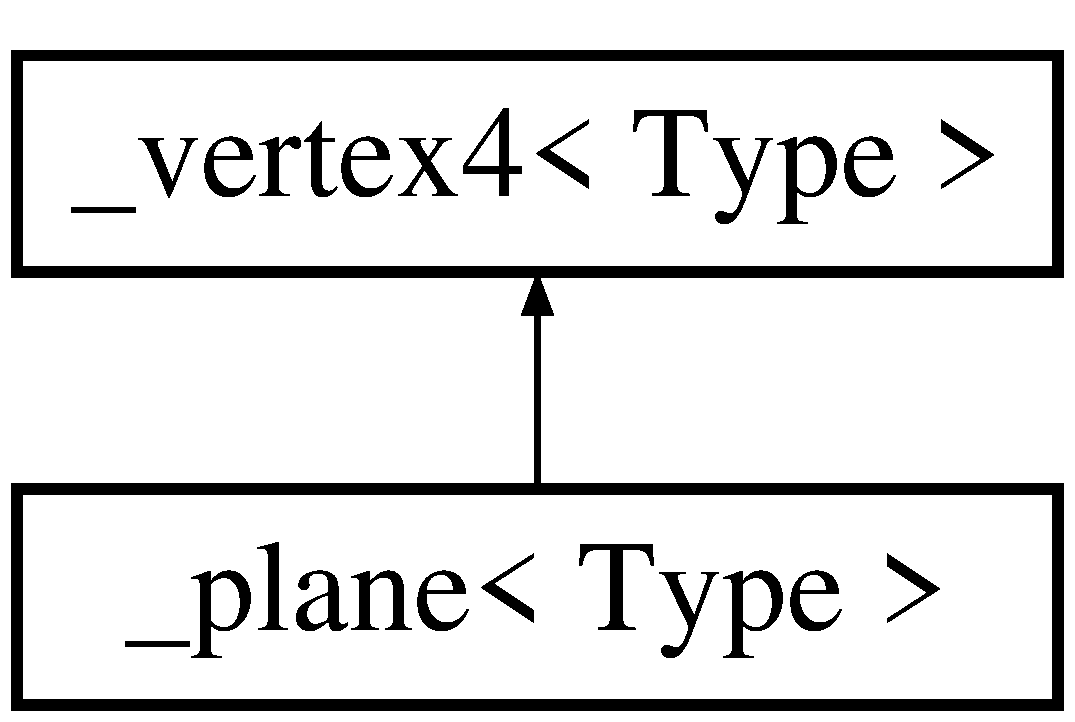
\includegraphics[height=2.000000cm]{class__plane}
\end{center}
\end{figure}
\subsection*{Public Member Functions}
\begin{DoxyCompactItemize}
\item 
\hyperlink{class__plane_abafcad1d36ec0cc2138d7a2fa7aa6246}{\+\_\+plane} (Type x1=0, Type y1=0, Type z1=0, Type w1=0)
\item 
\hyperlink{class__plane_ae7e80214cbb5d13c5f79715fec65490f}{\+\_\+plane} (const \hyperlink{class__vertex4}{\+\_\+vertex4}$<$ Type $>$ \&Vertex1)
\item 
\hyperlink{class__plane}{\+\_\+plane}$<$ Type $>$ \& \hyperlink{class__plane_add0ad8099978ac74fc3fa6c3ffe46847}{operator=} (\hyperlink{class__plane}{\+\_\+plane} \&Plane1)
\item 
int \hyperlink{class__plane_a291e8521201526dfe9133f595669121f}{compute\+\_\+coefficients} (\hyperlink{class__vertex3}{\+\_\+vertex3}$<$ Type $>$ Vertex1, \hyperlink{class__vertex3}{\+\_\+vertex3}$<$ Type $>$ Vertex2, \hyperlink{class__vertex3}{\+\_\+vertex3}$<$ Type $>$ Vertex3)
\item 
\hyperlink{vertex_8h_a2fc25f5ba8b6791cc76d4a49e06d6e8c}{\+\_\+vertex\+\_\+position} \hyperlink{class__plane_a6e4f08e519d6d15eaf667d7b5e9c515b}{compute\+\_\+vertex\+\_\+position} (\hyperlink{class__vertex3}{\+\_\+vertex3}$<$ Type $>$ Vertex1)
\item 
\hyperlink{class__vertex3}{\+\_\+vertex3}$<$ Type $>$ \hyperlink{class__plane_a9d74741f6fba658ad2a09f92145af878}{normal} ()
\item 
void \hyperlink{class__plane_ac73d74bef9360a384739e653809f36f0}{show\+\_\+values} ()
\end{DoxyCompactItemize}
\subsection*{Additional Inherited Members}


\subsection{Constructor \& Destructor Documentation}
\hypertarget{class__plane_abafcad1d36ec0cc2138d7a2fa7aa6246}{\index{\+\_\+plane@{\+\_\+plane}!\+\_\+plane@{\+\_\+plane}}
\index{\+\_\+plane@{\+\_\+plane}!\+\_\+plane@{\+\_\+plane}}
\subsubsection[{\+\_\+plane}]{\setlength{\rightskip}{0pt plus 5cm}template$<$class Type $>$ {\bf \+\_\+plane}$<$ Type $>$\+::{\bf \+\_\+plane} (
\begin{DoxyParamCaption}
\item[{Type}]{x1 = {\ttfamily 0}, }
\item[{Type}]{y1 = {\ttfamily 0}, }
\item[{Type}]{z1 = {\ttfamily 0}, }
\item[{Type}]{w1 = {\ttfamily 0}}
\end{DoxyParamCaption}
)}}\label{class__plane_abafcad1d36ec0cc2138d7a2fa7aa6246}
\hypertarget{class__plane_ae7e80214cbb5d13c5f79715fec65490f}{\index{\+\_\+plane@{\+\_\+plane}!\+\_\+plane@{\+\_\+plane}}
\index{\+\_\+plane@{\+\_\+plane}!\+\_\+plane@{\+\_\+plane}}
\subsubsection[{\+\_\+plane}]{\setlength{\rightskip}{0pt plus 5cm}template$<$class Type $>$ {\bf \+\_\+plane}$<$ Type $>$\+::{\bf \+\_\+plane} (
\begin{DoxyParamCaption}
\item[{const {\bf \+\_\+vertex4}$<$ Type $>$ \&}]{Vertex1}
\end{DoxyParamCaption}
)}}\label{class__plane_ae7e80214cbb5d13c5f79715fec65490f}


\subsection{Member Function Documentation}
\hypertarget{class__plane_a291e8521201526dfe9133f595669121f}{\index{\+\_\+plane@{\+\_\+plane}!compute\+\_\+coefficients@{compute\+\_\+coefficients}}
\index{compute\+\_\+coefficients@{compute\+\_\+coefficients}!\+\_\+plane@{\+\_\+plane}}
\subsubsection[{compute\+\_\+coefficients}]{\setlength{\rightskip}{0pt plus 5cm}template$<$class Type $>$ int {\bf \+\_\+plane}$<$ Type $>$\+::compute\+\_\+coefficients (
\begin{DoxyParamCaption}
\item[{{\bf \+\_\+vertex3}$<$ Type $>$}]{Vertex1, }
\item[{{\bf \+\_\+vertex3}$<$ Type $>$}]{Vertex2, }
\item[{{\bf \+\_\+vertex3}$<$ Type $>$}]{Vertex3}
\end{DoxyParamCaption}
)}}\label{class__plane_a291e8521201526dfe9133f595669121f}
\hypertarget{class__plane_a6e4f08e519d6d15eaf667d7b5e9c515b}{\index{\+\_\+plane@{\+\_\+plane}!compute\+\_\+vertex\+\_\+position@{compute\+\_\+vertex\+\_\+position}}
\index{compute\+\_\+vertex\+\_\+position@{compute\+\_\+vertex\+\_\+position}!\+\_\+plane@{\+\_\+plane}}
\subsubsection[{compute\+\_\+vertex\+\_\+position}]{\setlength{\rightskip}{0pt plus 5cm}template$<$class Type $>$ {\bf \+\_\+vertex\+\_\+position} {\bf \+\_\+plane}$<$ Type $>$\+::compute\+\_\+vertex\+\_\+position (
\begin{DoxyParamCaption}
\item[{{\bf \+\_\+vertex3}$<$ Type $>$}]{Vertex1}
\end{DoxyParamCaption}
)}}\label{class__plane_a6e4f08e519d6d15eaf667d7b5e9c515b}
\hypertarget{class__plane_a9d74741f6fba658ad2a09f92145af878}{\index{\+\_\+plane@{\+\_\+plane}!normal@{normal}}
\index{normal@{normal}!\+\_\+plane@{\+\_\+plane}}
\subsubsection[{normal}]{\setlength{\rightskip}{0pt plus 5cm}template$<$class Type $>$ {\bf \+\_\+vertex3}$<$ Type $>$ {\bf \+\_\+plane}$<$ Type $>$\+::normal (
\begin{DoxyParamCaption}
{}
\end{DoxyParamCaption}
)}}\label{class__plane_a9d74741f6fba658ad2a09f92145af878}
\hypertarget{class__plane_add0ad8099978ac74fc3fa6c3ffe46847}{\index{\+\_\+plane@{\+\_\+plane}!operator=@{operator=}}
\index{operator=@{operator=}!\+\_\+plane@{\+\_\+plane}}
\subsubsection[{operator=}]{\setlength{\rightskip}{0pt plus 5cm}template$<$class Type $>$ {\bf \+\_\+plane}$<$ Type $>$ \& {\bf \+\_\+plane}$<$ Type $>$\+::operator= (
\begin{DoxyParamCaption}
\item[{{\bf \+\_\+plane}$<$ Type $>$ \&}]{Plane1}
\end{DoxyParamCaption}
)}}\label{class__plane_add0ad8099978ac74fc3fa6c3ffe46847}
\hypertarget{class__plane_ac73d74bef9360a384739e653809f36f0}{\index{\+\_\+plane@{\+\_\+plane}!show\+\_\+values@{show\+\_\+values}}
\index{show\+\_\+values@{show\+\_\+values}!\+\_\+plane@{\+\_\+plane}}
\subsubsection[{show\+\_\+values}]{\setlength{\rightskip}{0pt plus 5cm}template$<$class Type$>$ void {\bf \+\_\+plane}$<$ Type $>$\+::show\+\_\+values (
\begin{DoxyParamCaption}
{}
\end{DoxyParamCaption}
)}}\label{class__plane_ac73d74bef9360a384739e653809f36f0}


The documentation for this class was generated from the following file\+:\begin{DoxyCompactItemize}
\item 
\hyperlink{vertex_8h}{vertex.\+h}\end{DoxyCompactItemize}

\hypertarget{class__vertex2}{\section{\+\_\+vertex2$<$ Type $>$ Class Template Reference}
\label{class__vertex2}\index{\+\_\+vertex2$<$ Type $>$@{\+\_\+vertex2$<$ Type $>$}}
}


{\ttfamily \#include $<$vertex.\+h$>$}

\subsection*{Public Member Functions}
\begin{DoxyCompactItemize}
\item 
\hyperlink{class__vertex2_a1256006c9ec2eb04b345e95dd338db43}{\+\_\+vertex2} (Type x1=0, Type y1=0)
\item 
\hyperlink{class__vertex2_a92d580fe161cf58b45366d3b79c364b0}{\+\_\+vertex2} (const \hyperlink{class__vertex2}{\+\_\+vertex2}$<$ Type $>$ \&Vertex1)
\item 
\hyperlink{class__vertex2_a3be9f6ba0f78200493137b29f257f809}{\+\_\+vertex2} (const \hyperlink{class__vertex3}{\+\_\+vertex3}$<$ Type $>$ \&Vertex1)
\item 
\hyperlink{class__vertex2_a8df74c05af0965f0a36788a3a08dea54}{\+\_\+vertex2} (const \hyperlink{class__vertex4}{\+\_\+vertex4}$<$ Type $>$ \&Vertex1)
\item 
\hyperlink{class__vertex2}{\+\_\+vertex2} \& \hyperlink{class__vertex2_a62782569f4c29f40518e286a1cb8685b}{operator()} (Type x1, Type y1)
\item 
\hyperlink{class__vertex2}{\+\_\+vertex2} \& \hyperlink{class__vertex2_a8177cc59f40d48e3ef5fec43f88ba800}{operator()} (Type $\ast$Vertices1)
\item 
\hyperlink{class__vertex2}{\+\_\+vertex2} \& \hyperlink{class__vertex2_a8a091f80e485e6d8cff9ee2184f4a702}{operator()} (const \hyperlink{class__vertex2}{\+\_\+vertex2}$<$ Type $>$ \&Vertex1)
\item 
\hyperlink{class__vertex2}{\+\_\+vertex2} \& \hyperlink{class__vertex2_a8c33125f66c38434e5c7a6a910314468}{operator()} (const \hyperlink{class__vertex3}{\+\_\+vertex3}$<$ Type $>$ \&Vertex1)
\item 
\hyperlink{class__vertex2}{\+\_\+vertex2} \& \hyperlink{class__vertex2_a266c820652c758060707431cba08e186}{operator()} (const \hyperlink{class__vertex4}{\+\_\+vertex4}$<$ Type $>$ \&Vertex1)
\item 
\hyperlink{class__vertex2}{\+\_\+vertex2} \& \hyperlink{class__vertex2_a38bdd225746becf2db55ea7222529f83}{operator=} (const \hyperlink{class__vertex2}{\+\_\+vertex2}$<$ Type $>$ \&Vertex1)
\item 
\hyperlink{class__vertex2}{\+\_\+vertex2} \& \hyperlink{class__vertex2_a99100f6414212d660b47ef757fbda530}{operator=} (const \hyperlink{class__vertex3}{\+\_\+vertex3}$<$ Type $>$ \&Vertex1)
\item 
\hyperlink{class__vertex2}{\+\_\+vertex2} \& \hyperlink{class__vertex2_a721bced51179d5eb8e4f2b55d6575cbf}{operator=} (const \hyperlink{class__vertex4}{\+\_\+vertex4}$<$ Type $>$ \&Vertex1)
\item 
\hyperlink{class__vertex2}{\+\_\+vertex2} \& \hyperlink{class__vertex2_a93c58d5bf73deaaa373529db52c86279}{operator=} (Type $\ast$Vertices1)
\item 
\hyperlink{class__vertex2}{\+\_\+vertex2} \hyperlink{class__vertex2_ae1910f3f68a0d24611ff0d6d266ee58b}{operator+} (const \hyperlink{class__vertex2}{\+\_\+vertex2}$<$ Type $>$ \&Vertex1)
\item 
\hyperlink{class__vertex2}{\+\_\+vertex2} \& \hyperlink{class__vertex2_ae16f5ae01aa44a8564abba7d2a45f403}{operator+=} (const \hyperlink{class__vertex2}{\+\_\+vertex2}$<$ Type $>$ \&Vertex1)
\item 
\hyperlink{class__vertex2}{\+\_\+vertex2} \hyperlink{class__vertex2_a83231d384db1e1da9630e96296202cfc}{operator-\/} (const \hyperlink{class__vertex2}{\+\_\+vertex2}$<$ Type $>$ \&Vertex1)
\item 
\hyperlink{class__vertex2}{\+\_\+vertex2} \& \hyperlink{class__vertex2_a5268d2764acca259d8d4f1258fa75ae4}{operator-\/=} (const \hyperlink{class__vertex2}{\+\_\+vertex2}$<$ Type $>$ \&Vertex1)
\item 
\hyperlink{class__vertex2}{\+\_\+vertex2} \hyperlink{class__vertex2_aab7c18e4b66c030ea673d95dd02b3166}{operator$\ast$} (Type Value)
\item 
\hyperlink{class__vertex2}{\+\_\+vertex2} \& \hyperlink{class__vertex2_a30996bf8e5b2791fd100614376843c7c}{operator$\ast$=} (Type Value)
\item 
\hyperlink{class__vertex2}{\+\_\+vertex2} \hyperlink{class__vertex2_a8d881ad9953a6f3239eae673357668b1}{operator/} (Type Value)
\item 
\hyperlink{class__vertex2}{\+\_\+vertex2} \& \hyperlink{class__vertex2_af5073a4eadd0a45ca1ba87c0e2f3ae3c}{operator/=} (Type Value)
\item 
Type \hyperlink{class__vertex2_aec1d371dfc0e540cc26f926f21554826}{dot\+\_\+product} (const \hyperlink{class__vertex2}{\+\_\+vertex2}$<$ Type $>$ \&Vertex1)
\item 
bool \hyperlink{class__vertex2_a557b9518ccdd4534e246770f73a7e556}{operator==} (const \hyperlink{class__vertex2}{\+\_\+vertex2}$<$ Type $>$ \&Vertex1)
\item 
bool \hyperlink{class__vertex2_abd28310390cfac783f29354a0ea0a8d3}{operator!=} (const \hyperlink{class__vertex2}{\+\_\+vertex2}$<$ Type $>$ \&Vertex1)
\item 
\hyperlink{class__vertex2}{\+\_\+vertex2} \& \hyperlink{class__vertex2_a300c0eeffd16df52f5a0990a1c086562}{normalize} ()
\item 
double \hyperlink{class__vertex2_ab19da68cecb3e4316edba46c2114a63b}{module} ()
\item 
\hyperlink{class__vertex2}{\+\_\+vertex2} \hyperlink{class__vertex2_ac00409cafb646e6cba805a7759d7db69}{clone} ()
\item 
Type \& \hyperlink{class__vertex2_a0fe2648c8afb5db0202af70f1d94bdb7}{operator\mbox{[}$\,$\mbox{]}} (int Position)
\item 
void \hyperlink{class__vertex2_a80da2494e943c19cc1e5f68191d455f5}{show\+\_\+values} ()
\end{DoxyCompactItemize}
\subsection*{Public Attributes}
\begin{DoxyCompactItemize}
\item 
\begin{tabbing}
xx\=xx\=xx\=xx\=xx\=xx\=xx\=xx\=xx\=\kill
union \{\\
\>Type \hyperlink{class__vertex2_a34050e835b9dafb02d5a61381bbaa434}{x}\\
\>Type \hyperlink{class__vertex2_a5a404037c59e0d4c2af8ba301e006cef}{r}\\
\>Type \hyperlink{class__vertex2_a4d6ed656629478ac2f367bec00589ec0}{s}\\
\>Type \hyperlink{class__vertex2_aba4452e10ea646649c3fd6c9cec1c89e}{\_0}\\
\>Type \hyperlink{class__vertex2_aa0d662a46c73e4c737fe9c09b54412c5}{row}\\
\}; \\

\end{tabbing}\item 
\begin{tabbing}
xx\=xx\=xx\=xx\=xx\=xx\=xx\=xx\=xx\=\kill
union \{\\
\>Type \hyperlink{class__vertex2_a4988efe986242839b52ce5c91889325e}{y}\\
\>Type \hyperlink{class__vertex2_aefb25eeec2261091016c3cfe508fdaaa}{g}\\
\>Type \hyperlink{class__vertex2_a64f0152747b02f799880ee51111f6316}{t}\\
\>Type \hyperlink{class__vertex2_a2f4d1d0369130356ebdf797b6da78bb8}{\_1}\\
\>Type \hyperlink{class__vertex2_a522c14fc32a2228789325db485217eeb}{col}\\
\}; \\

\end{tabbing}\end{DoxyCompactItemize}


\subsection{Constructor \& Destructor Documentation}
\hypertarget{class__vertex2_a1256006c9ec2eb04b345e95dd338db43}{\index{\+\_\+vertex2@{\+\_\+vertex2}!\+\_\+vertex2@{\+\_\+vertex2}}
\index{\+\_\+vertex2@{\+\_\+vertex2}!\+\_\+vertex2@{\+\_\+vertex2}}
\subsubsection[{\+\_\+vertex2}]{\setlength{\rightskip}{0pt plus 5cm}template$<$class Type $>$ {\bf \+\_\+vertex2}$<$ Type $>$\+::{\bf \+\_\+vertex2} (
\begin{DoxyParamCaption}
\item[{Type}]{x1 = {\ttfamily 0}, }
\item[{Type}]{y1 = {\ttfamily 0}}
\end{DoxyParamCaption}
)}}\label{class__vertex2_a1256006c9ec2eb04b345e95dd338db43}
\hypertarget{class__vertex2_a92d580fe161cf58b45366d3b79c364b0}{\index{\+\_\+vertex2@{\+\_\+vertex2}!\+\_\+vertex2@{\+\_\+vertex2}}
\index{\+\_\+vertex2@{\+\_\+vertex2}!\+\_\+vertex2@{\+\_\+vertex2}}
\subsubsection[{\+\_\+vertex2}]{\setlength{\rightskip}{0pt plus 5cm}template$<$class Type $>$ {\bf \+\_\+vertex2}$<$ Type $>$\+::{\bf \+\_\+vertex2} (
\begin{DoxyParamCaption}
\item[{const {\bf \+\_\+vertex2}$<$ Type $>$ \&}]{Vertex1}
\end{DoxyParamCaption}
)}}\label{class__vertex2_a92d580fe161cf58b45366d3b79c364b0}
\hypertarget{class__vertex2_a3be9f6ba0f78200493137b29f257f809}{\index{\+\_\+vertex2@{\+\_\+vertex2}!\+\_\+vertex2@{\+\_\+vertex2}}
\index{\+\_\+vertex2@{\+\_\+vertex2}!\+\_\+vertex2@{\+\_\+vertex2}}
\subsubsection[{\+\_\+vertex2}]{\setlength{\rightskip}{0pt plus 5cm}template$<$class Type $>$ {\bf \+\_\+vertex2}$<$ Type $>$\+::{\bf \+\_\+vertex2} (
\begin{DoxyParamCaption}
\item[{const {\bf \+\_\+vertex3}$<$ Type $>$ \&}]{Vertex1}
\end{DoxyParamCaption}
)}}\label{class__vertex2_a3be9f6ba0f78200493137b29f257f809}
\hypertarget{class__vertex2_a8df74c05af0965f0a36788a3a08dea54}{\index{\+\_\+vertex2@{\+\_\+vertex2}!\+\_\+vertex2@{\+\_\+vertex2}}
\index{\+\_\+vertex2@{\+\_\+vertex2}!\+\_\+vertex2@{\+\_\+vertex2}}
\subsubsection[{\+\_\+vertex2}]{\setlength{\rightskip}{0pt plus 5cm}template$<$class Type $>$ {\bf \+\_\+vertex2}$<$ Type $>$\+::{\bf \+\_\+vertex2} (
\begin{DoxyParamCaption}
\item[{const {\bf \+\_\+vertex4}$<$ Type $>$ \&}]{Vertex1}
\end{DoxyParamCaption}
)}}\label{class__vertex2_a8df74c05af0965f0a36788a3a08dea54}


\subsection{Member Function Documentation}
\hypertarget{class__vertex2_ac00409cafb646e6cba805a7759d7db69}{\index{\+\_\+vertex2@{\+\_\+vertex2}!clone@{clone}}
\index{clone@{clone}!\+\_\+vertex2@{\+\_\+vertex2}}
\subsubsection[{clone}]{\setlength{\rightskip}{0pt plus 5cm}template$<$class Type$>$ {\bf \+\_\+vertex2} {\bf \+\_\+vertex2}$<$ Type $>$\+::clone (
\begin{DoxyParamCaption}
{}
\end{DoxyParamCaption}
)\hspace{0.3cm}{\ttfamily [inline]}}}\label{class__vertex2_ac00409cafb646e6cba805a7759d7db69}
\hypertarget{class__vertex2_aec1d371dfc0e540cc26f926f21554826}{\index{\+\_\+vertex2@{\+\_\+vertex2}!dot\+\_\+product@{dot\+\_\+product}}
\index{dot\+\_\+product@{dot\+\_\+product}!\+\_\+vertex2@{\+\_\+vertex2}}
\subsubsection[{dot\+\_\+product}]{\setlength{\rightskip}{0pt plus 5cm}template$<$class Type$>$ Type {\bf \+\_\+vertex2}$<$ Type $>$\+::dot\+\_\+product (
\begin{DoxyParamCaption}
\item[{const {\bf \+\_\+vertex2}$<$ Type $>$ \&}]{Vertex1}
\end{DoxyParamCaption}
)\hspace{0.3cm}{\ttfamily [inline]}}}\label{class__vertex2_aec1d371dfc0e540cc26f926f21554826}
\hypertarget{class__vertex2_ab19da68cecb3e4316edba46c2114a63b}{\index{\+\_\+vertex2@{\+\_\+vertex2}!module@{module}}
\index{module@{module}!\+\_\+vertex2@{\+\_\+vertex2}}
\subsubsection[{module}]{\setlength{\rightskip}{0pt plus 5cm}template$<$class Type$>$ double {\bf \+\_\+vertex2}$<$ Type $>$\+::module (
\begin{DoxyParamCaption}
{}
\end{DoxyParamCaption}
)\hspace{0.3cm}{\ttfamily [inline]}}}\label{class__vertex2_ab19da68cecb3e4316edba46c2114a63b}
\hypertarget{class__vertex2_a300c0eeffd16df52f5a0990a1c086562}{\index{\+\_\+vertex2@{\+\_\+vertex2}!normalize@{normalize}}
\index{normalize@{normalize}!\+\_\+vertex2@{\+\_\+vertex2}}
\subsubsection[{normalize}]{\setlength{\rightskip}{0pt plus 5cm}template$<$class Type $>$ {\bf \+\_\+vertex2}$<$ Type $>$ \& {\bf \+\_\+vertex2}$<$ Type $>$\+::normalize (
\begin{DoxyParamCaption}
{}
\end{DoxyParamCaption}
)}}\label{class__vertex2_a300c0eeffd16df52f5a0990a1c086562}
\hypertarget{class__vertex2_abd28310390cfac783f29354a0ea0a8d3}{\index{\+\_\+vertex2@{\+\_\+vertex2}!operator"!=@{operator"!=}}
\index{operator"!=@{operator"!=}!\+\_\+vertex2@{\+\_\+vertex2}}
\subsubsection[{operator"!=}]{\setlength{\rightskip}{0pt plus 5cm}template$<$class Type $>$ bool {\bf \+\_\+vertex2}$<$ Type $>$\+::operator!= (
\begin{DoxyParamCaption}
\item[{const {\bf \+\_\+vertex2}$<$ Type $>$ \&}]{Vertex1}
\end{DoxyParamCaption}
)}}\label{class__vertex2_abd28310390cfac783f29354a0ea0a8d3}
\hypertarget{class__vertex2_a62782569f4c29f40518e286a1cb8685b}{\index{\+\_\+vertex2@{\+\_\+vertex2}!operator()@{operator()}}
\index{operator()@{operator()}!\+\_\+vertex2@{\+\_\+vertex2}}
\subsubsection[{operator()}]{\setlength{\rightskip}{0pt plus 5cm}template$<$class Type $>$ {\bf \+\_\+vertex2}$<$ Type $>$ \& {\bf \+\_\+vertex2}$<$ Type $>$\+::operator() (
\begin{DoxyParamCaption}
\item[{Type}]{x1, }
\item[{Type}]{y1}
\end{DoxyParamCaption}
)}}\label{class__vertex2_a62782569f4c29f40518e286a1cb8685b}
\hypertarget{class__vertex2_a8177cc59f40d48e3ef5fec43f88ba800}{\index{\+\_\+vertex2@{\+\_\+vertex2}!operator()@{operator()}}
\index{operator()@{operator()}!\+\_\+vertex2@{\+\_\+vertex2}}
\subsubsection[{operator()}]{\setlength{\rightskip}{0pt plus 5cm}template$<$class Type $>$ {\bf \+\_\+vertex2}$<$ Type $>$ \& {\bf \+\_\+vertex2}$<$ Type $>$\+::operator() (
\begin{DoxyParamCaption}
\item[{Type $\ast$}]{Vertices1}
\end{DoxyParamCaption}
)}}\label{class__vertex2_a8177cc59f40d48e3ef5fec43f88ba800}
\hypertarget{class__vertex2_a8a091f80e485e6d8cff9ee2184f4a702}{\index{\+\_\+vertex2@{\+\_\+vertex2}!operator()@{operator()}}
\index{operator()@{operator()}!\+\_\+vertex2@{\+\_\+vertex2}}
\subsubsection[{operator()}]{\setlength{\rightskip}{0pt plus 5cm}template$<$class Type $>$ {\bf \+\_\+vertex2}$<$ Type $>$ \& {\bf \+\_\+vertex2}$<$ Type $>$\+::operator() (
\begin{DoxyParamCaption}
\item[{const {\bf \+\_\+vertex2}$<$ Type $>$ \&}]{Vertex1}
\end{DoxyParamCaption}
)}}\label{class__vertex2_a8a091f80e485e6d8cff9ee2184f4a702}
\hypertarget{class__vertex2_a8c33125f66c38434e5c7a6a910314468}{\index{\+\_\+vertex2@{\+\_\+vertex2}!operator()@{operator()}}
\index{operator()@{operator()}!\+\_\+vertex2@{\+\_\+vertex2}}
\subsubsection[{operator()}]{\setlength{\rightskip}{0pt plus 5cm}template$<$class Type $>$ {\bf \+\_\+vertex2}$<$ Type $>$ \& {\bf \+\_\+vertex2}$<$ Type $>$\+::operator() (
\begin{DoxyParamCaption}
\item[{const {\bf \+\_\+vertex3}$<$ Type $>$ \&}]{Vertex1}
\end{DoxyParamCaption}
)}}\label{class__vertex2_a8c33125f66c38434e5c7a6a910314468}
\hypertarget{class__vertex2_a266c820652c758060707431cba08e186}{\index{\+\_\+vertex2@{\+\_\+vertex2}!operator()@{operator()}}
\index{operator()@{operator()}!\+\_\+vertex2@{\+\_\+vertex2}}
\subsubsection[{operator()}]{\setlength{\rightskip}{0pt plus 5cm}template$<$class Type $>$ {\bf \+\_\+vertex2}$<$ Type $>$ \& {\bf \+\_\+vertex2}$<$ Type $>$\+::operator() (
\begin{DoxyParamCaption}
\item[{const {\bf \+\_\+vertex4}$<$ Type $>$ \&}]{Vertex1}
\end{DoxyParamCaption}
)}}\label{class__vertex2_a266c820652c758060707431cba08e186}
\hypertarget{class__vertex2_aab7c18e4b66c030ea673d95dd02b3166}{\index{\+\_\+vertex2@{\+\_\+vertex2}!operator$\ast$@{operator$\ast$}}
\index{operator$\ast$@{operator$\ast$}!\+\_\+vertex2@{\+\_\+vertex2}}
\subsubsection[{operator$\ast$}]{\setlength{\rightskip}{0pt plus 5cm}template$<$class Type $>$ {\bf \+\_\+vertex2}$<$ Type $>$ {\bf \+\_\+vertex2}$<$ Type $>$\+::operator$\ast$ (
\begin{DoxyParamCaption}
\item[{Type}]{Value}
\end{DoxyParamCaption}
)}}\label{class__vertex2_aab7c18e4b66c030ea673d95dd02b3166}
\hypertarget{class__vertex2_a30996bf8e5b2791fd100614376843c7c}{\index{\+\_\+vertex2@{\+\_\+vertex2}!operator$\ast$=@{operator$\ast$=}}
\index{operator$\ast$=@{operator$\ast$=}!\+\_\+vertex2@{\+\_\+vertex2}}
\subsubsection[{operator$\ast$=}]{\setlength{\rightskip}{0pt plus 5cm}template$<$class Type $>$ {\bf \+\_\+vertex2}$<$ Type $>$ \& {\bf \+\_\+vertex2}$<$ Type $>$\+::operator$\ast$= (
\begin{DoxyParamCaption}
\item[{Type}]{Value}
\end{DoxyParamCaption}
)}}\label{class__vertex2_a30996bf8e5b2791fd100614376843c7c}
\hypertarget{class__vertex2_ae1910f3f68a0d24611ff0d6d266ee58b}{\index{\+\_\+vertex2@{\+\_\+vertex2}!operator+@{operator+}}
\index{operator+@{operator+}!\+\_\+vertex2@{\+\_\+vertex2}}
\subsubsection[{operator+}]{\setlength{\rightskip}{0pt plus 5cm}template$<$class Type $>$ {\bf \+\_\+vertex2}$<$ Type $>$ {\bf \+\_\+vertex2}$<$ Type $>$\+::operator+ (
\begin{DoxyParamCaption}
\item[{const {\bf \+\_\+vertex2}$<$ Type $>$ \&}]{Vertex1}
\end{DoxyParamCaption}
)}}\label{class__vertex2_ae1910f3f68a0d24611ff0d6d266ee58b}
\hypertarget{class__vertex2_ae16f5ae01aa44a8564abba7d2a45f403}{\index{\+\_\+vertex2@{\+\_\+vertex2}!operator+=@{operator+=}}
\index{operator+=@{operator+=}!\+\_\+vertex2@{\+\_\+vertex2}}
\subsubsection[{operator+=}]{\setlength{\rightskip}{0pt plus 5cm}template$<$class Type $>$ {\bf \+\_\+vertex2}$<$ Type $>$ \& {\bf \+\_\+vertex2}$<$ Type $>$\+::operator+= (
\begin{DoxyParamCaption}
\item[{const {\bf \+\_\+vertex2}$<$ Type $>$ \&}]{Vertex1}
\end{DoxyParamCaption}
)}}\label{class__vertex2_ae16f5ae01aa44a8564abba7d2a45f403}
\hypertarget{class__vertex2_a83231d384db1e1da9630e96296202cfc}{\index{\+\_\+vertex2@{\+\_\+vertex2}!operator-\/@{operator-\/}}
\index{operator-\/@{operator-\/}!\+\_\+vertex2@{\+\_\+vertex2}}
\subsubsection[{operator-\/}]{\setlength{\rightskip}{0pt plus 5cm}template$<$class Type $>$ {\bf \+\_\+vertex2}$<$ Type $>$ {\bf \+\_\+vertex2}$<$ Type $>$\+::operator-\/ (
\begin{DoxyParamCaption}
\item[{const {\bf \+\_\+vertex2}$<$ Type $>$ \&}]{Vertex1}
\end{DoxyParamCaption}
)}}\label{class__vertex2_a83231d384db1e1da9630e96296202cfc}
\hypertarget{class__vertex2_a5268d2764acca259d8d4f1258fa75ae4}{\index{\+\_\+vertex2@{\+\_\+vertex2}!operator-\/=@{operator-\/=}}
\index{operator-\/=@{operator-\/=}!\+\_\+vertex2@{\+\_\+vertex2}}
\subsubsection[{operator-\/=}]{\setlength{\rightskip}{0pt plus 5cm}template$<$class Type $>$ {\bf \+\_\+vertex2}$<$ Type $>$ \& {\bf \+\_\+vertex2}$<$ Type $>$\+::operator-\/= (
\begin{DoxyParamCaption}
\item[{const {\bf \+\_\+vertex2}$<$ Type $>$ \&}]{Vertex1}
\end{DoxyParamCaption}
)}}\label{class__vertex2_a5268d2764acca259d8d4f1258fa75ae4}
\hypertarget{class__vertex2_a8d881ad9953a6f3239eae673357668b1}{\index{\+\_\+vertex2@{\+\_\+vertex2}!operator/@{operator/}}
\index{operator/@{operator/}!\+\_\+vertex2@{\+\_\+vertex2}}
\subsubsection[{operator/}]{\setlength{\rightskip}{0pt plus 5cm}template$<$class Type $>$ {\bf \+\_\+vertex2}$<$ Type $>$ {\bf \+\_\+vertex2}$<$ Type $>$\+::operator/ (
\begin{DoxyParamCaption}
\item[{Type}]{Value}
\end{DoxyParamCaption}
)}}\label{class__vertex2_a8d881ad9953a6f3239eae673357668b1}
\hypertarget{class__vertex2_af5073a4eadd0a45ca1ba87c0e2f3ae3c}{\index{\+\_\+vertex2@{\+\_\+vertex2}!operator/=@{operator/=}}
\index{operator/=@{operator/=}!\+\_\+vertex2@{\+\_\+vertex2}}
\subsubsection[{operator/=}]{\setlength{\rightskip}{0pt plus 5cm}template$<$class Type $>$ {\bf \+\_\+vertex2}$<$ Type $>$ \& {\bf \+\_\+vertex2}$<$ Type $>$\+::operator/= (
\begin{DoxyParamCaption}
\item[{Type}]{Value}
\end{DoxyParamCaption}
)}}\label{class__vertex2_af5073a4eadd0a45ca1ba87c0e2f3ae3c}
\hypertarget{class__vertex2_a38bdd225746becf2db55ea7222529f83}{\index{\+\_\+vertex2@{\+\_\+vertex2}!operator=@{operator=}}
\index{operator=@{operator=}!\+\_\+vertex2@{\+\_\+vertex2}}
\subsubsection[{operator=}]{\setlength{\rightskip}{0pt plus 5cm}template$<$class Type $>$ {\bf \+\_\+vertex2}$<$ Type $>$ \& {\bf \+\_\+vertex2}$<$ Type $>$\+::operator= (
\begin{DoxyParamCaption}
\item[{const {\bf \+\_\+vertex2}$<$ Type $>$ \&}]{Vertex1}
\end{DoxyParamCaption}
)}}\label{class__vertex2_a38bdd225746becf2db55ea7222529f83}
\hypertarget{class__vertex2_a99100f6414212d660b47ef757fbda530}{\index{\+\_\+vertex2@{\+\_\+vertex2}!operator=@{operator=}}
\index{operator=@{operator=}!\+\_\+vertex2@{\+\_\+vertex2}}
\subsubsection[{operator=}]{\setlength{\rightskip}{0pt plus 5cm}template$<$class Type $>$ {\bf \+\_\+vertex2}$<$ Type $>$ \& {\bf \+\_\+vertex2}$<$ Type $>$\+::operator= (
\begin{DoxyParamCaption}
\item[{const {\bf \+\_\+vertex3}$<$ Type $>$ \&}]{Vertex1}
\end{DoxyParamCaption}
)}}\label{class__vertex2_a99100f6414212d660b47ef757fbda530}
\hypertarget{class__vertex2_a721bced51179d5eb8e4f2b55d6575cbf}{\index{\+\_\+vertex2@{\+\_\+vertex2}!operator=@{operator=}}
\index{operator=@{operator=}!\+\_\+vertex2@{\+\_\+vertex2}}
\subsubsection[{operator=}]{\setlength{\rightskip}{0pt plus 5cm}template$<$class Type $>$ {\bf \+\_\+vertex2}$<$ Type $>$ \& {\bf \+\_\+vertex2}$<$ Type $>$\+::operator= (
\begin{DoxyParamCaption}
\item[{const {\bf \+\_\+vertex4}$<$ Type $>$ \&}]{Vertex1}
\end{DoxyParamCaption}
)}}\label{class__vertex2_a721bced51179d5eb8e4f2b55d6575cbf}
\hypertarget{class__vertex2_a93c58d5bf73deaaa373529db52c86279}{\index{\+\_\+vertex2@{\+\_\+vertex2}!operator=@{operator=}}
\index{operator=@{operator=}!\+\_\+vertex2@{\+\_\+vertex2}}
\subsubsection[{operator=}]{\setlength{\rightskip}{0pt plus 5cm}template$<$class Type $>$ {\bf \+\_\+vertex2}$<$ Type $>$ \& {\bf \+\_\+vertex2}$<$ Type $>$\+::operator= (
\begin{DoxyParamCaption}
\item[{Type $\ast$}]{Vertices1}
\end{DoxyParamCaption}
)}}\label{class__vertex2_a93c58d5bf73deaaa373529db52c86279}
\hypertarget{class__vertex2_a557b9518ccdd4534e246770f73a7e556}{\index{\+\_\+vertex2@{\+\_\+vertex2}!operator==@{operator==}}
\index{operator==@{operator==}!\+\_\+vertex2@{\+\_\+vertex2}}
\subsubsection[{operator==}]{\setlength{\rightskip}{0pt plus 5cm}template$<$class Type $>$ bool {\bf \+\_\+vertex2}$<$ Type $>$\+::operator== (
\begin{DoxyParamCaption}
\item[{const {\bf \+\_\+vertex2}$<$ Type $>$ \&}]{Vertex1}
\end{DoxyParamCaption}
)}}\label{class__vertex2_a557b9518ccdd4534e246770f73a7e556}
\hypertarget{class__vertex2_a0fe2648c8afb5db0202af70f1d94bdb7}{\index{\+\_\+vertex2@{\+\_\+vertex2}!operator\mbox{[}$\,$\mbox{]}@{operator[]}}
\index{operator\mbox{[}$\,$\mbox{]}@{operator[]}!\+\_\+vertex2@{\+\_\+vertex2}}
\subsubsection[{operator[]}]{\setlength{\rightskip}{0pt plus 5cm}template$<$class Type$>$ Type\& {\bf \+\_\+vertex2}$<$ Type $>$\+::operator\mbox{[}$\,$\mbox{]} (
\begin{DoxyParamCaption}
\item[{int}]{Position}
\end{DoxyParamCaption}
)\hspace{0.3cm}{\ttfamily [inline]}}}\label{class__vertex2_a0fe2648c8afb5db0202af70f1d94bdb7}
\hypertarget{class__vertex2_a80da2494e943c19cc1e5f68191d455f5}{\index{\+\_\+vertex2@{\+\_\+vertex2}!show\+\_\+values@{show\+\_\+values}}
\index{show\+\_\+values@{show\+\_\+values}!\+\_\+vertex2@{\+\_\+vertex2}}
\subsubsection[{show\+\_\+values}]{\setlength{\rightskip}{0pt plus 5cm}template$<$class Type $>$ void {\bf \+\_\+vertex2}$<$ Type $>$\+::show\+\_\+values (
\begin{DoxyParamCaption}
{}
\end{DoxyParamCaption}
)}}\label{class__vertex2_a80da2494e943c19cc1e5f68191d455f5}


\subsection{Member Data Documentation}
\hypertarget{class__vertex2_af41de4f01565ae1825909a8b8d1a9c75}{\subsubsection[{"@1}]{\setlength{\rightskip}{0pt plus 5cm}union \{ ... \} }}\label{class__vertex2_af41de4f01565ae1825909a8b8d1a9c75}
\hypertarget{class__vertex2_a0337e24bb2631d3de2e6fc12dcc9c5b0}{\subsubsection[{"@3}]{\setlength{\rightskip}{0pt plus 5cm}union \{ ... \} }}\label{class__vertex2_a0337e24bb2631d3de2e6fc12dcc9c5b0}
\hypertarget{class__vertex2_aba4452e10ea646649c3fd6c9cec1c89e}{\index{\+\_\+vertex2@{\+\_\+vertex2}!\+\_\+0@{\+\_\+0}}
\index{\+\_\+0@{\+\_\+0}!\+\_\+vertex2@{\+\_\+vertex2}}
\subsubsection[{\+\_\+0}]{\setlength{\rightskip}{0pt plus 5cm}template$<$class Type$>$ Type {\bf \+\_\+vertex2}$<$ Type $>$\+::\+\_\+0}}\label{class__vertex2_aba4452e10ea646649c3fd6c9cec1c89e}
\hypertarget{class__vertex2_a2f4d1d0369130356ebdf797b6da78bb8}{\index{\+\_\+vertex2@{\+\_\+vertex2}!\+\_\+1@{\+\_\+1}}
\index{\+\_\+1@{\+\_\+1}!\+\_\+vertex2@{\+\_\+vertex2}}
\subsubsection[{\+\_\+1}]{\setlength{\rightskip}{0pt plus 5cm}template$<$class Type$>$ Type {\bf \+\_\+vertex2}$<$ Type $>$\+::\+\_\+1}}\label{class__vertex2_a2f4d1d0369130356ebdf797b6da78bb8}
\hypertarget{class__vertex2_a522c14fc32a2228789325db485217eeb}{\index{\+\_\+vertex2@{\+\_\+vertex2}!col@{col}}
\index{col@{col}!\+\_\+vertex2@{\+\_\+vertex2}}
\subsubsection[{col}]{\setlength{\rightskip}{0pt plus 5cm}template$<$class Type$>$ Type {\bf \+\_\+vertex2}$<$ Type $>$\+::col}}\label{class__vertex2_a522c14fc32a2228789325db485217eeb}
\hypertarget{class__vertex2_aefb25eeec2261091016c3cfe508fdaaa}{\index{\+\_\+vertex2@{\+\_\+vertex2}!g@{g}}
\index{g@{g}!\+\_\+vertex2@{\+\_\+vertex2}}
\subsubsection[{g}]{\setlength{\rightskip}{0pt plus 5cm}template$<$class Type$>$ Type {\bf \+\_\+vertex2}$<$ Type $>$\+::g}}\label{class__vertex2_aefb25eeec2261091016c3cfe508fdaaa}
\hypertarget{class__vertex2_a5a404037c59e0d4c2af8ba301e006cef}{\index{\+\_\+vertex2@{\+\_\+vertex2}!r@{r}}
\index{r@{r}!\+\_\+vertex2@{\+\_\+vertex2}}
\subsubsection[{r}]{\setlength{\rightskip}{0pt plus 5cm}template$<$class Type$>$ Type {\bf \+\_\+vertex2}$<$ Type $>$\+::r}}\label{class__vertex2_a5a404037c59e0d4c2af8ba301e006cef}
\hypertarget{class__vertex2_aa0d662a46c73e4c737fe9c09b54412c5}{\index{\+\_\+vertex2@{\+\_\+vertex2}!row@{row}}
\index{row@{row}!\+\_\+vertex2@{\+\_\+vertex2}}
\subsubsection[{row}]{\setlength{\rightskip}{0pt plus 5cm}template$<$class Type$>$ Type {\bf \+\_\+vertex2}$<$ Type $>$\+::row}}\label{class__vertex2_aa0d662a46c73e4c737fe9c09b54412c5}
\hypertarget{class__vertex2_a4d6ed656629478ac2f367bec00589ec0}{\index{\+\_\+vertex2@{\+\_\+vertex2}!s@{s}}
\index{s@{s}!\+\_\+vertex2@{\+\_\+vertex2}}
\subsubsection[{s}]{\setlength{\rightskip}{0pt plus 5cm}template$<$class Type$>$ Type {\bf \+\_\+vertex2}$<$ Type $>$\+::s}}\label{class__vertex2_a4d6ed656629478ac2f367bec00589ec0}
\hypertarget{class__vertex2_a64f0152747b02f799880ee51111f6316}{\index{\+\_\+vertex2@{\+\_\+vertex2}!t@{t}}
\index{t@{t}!\+\_\+vertex2@{\+\_\+vertex2}}
\subsubsection[{t}]{\setlength{\rightskip}{0pt plus 5cm}template$<$class Type$>$ Type {\bf \+\_\+vertex2}$<$ Type $>$\+::t}}\label{class__vertex2_a64f0152747b02f799880ee51111f6316}
\hypertarget{class__vertex2_a34050e835b9dafb02d5a61381bbaa434}{\index{\+\_\+vertex2@{\+\_\+vertex2}!x@{x}}
\index{x@{x}!\+\_\+vertex2@{\+\_\+vertex2}}
\subsubsection[{x}]{\setlength{\rightskip}{0pt plus 5cm}template$<$class Type$>$ Type {\bf \+\_\+vertex2}$<$ Type $>$\+::x}}\label{class__vertex2_a34050e835b9dafb02d5a61381bbaa434}
\hypertarget{class__vertex2_a4988efe986242839b52ce5c91889325e}{\index{\+\_\+vertex2@{\+\_\+vertex2}!y@{y}}
\index{y@{y}!\+\_\+vertex2@{\+\_\+vertex2}}
\subsubsection[{y}]{\setlength{\rightskip}{0pt plus 5cm}template$<$class Type$>$ Type {\bf \+\_\+vertex2}$<$ Type $>$\+::y}}\label{class__vertex2_a4988efe986242839b52ce5c91889325e}


The documentation for this class was generated from the following file\+:\begin{DoxyCompactItemize}
\item 
\hyperlink{vertex_8h}{vertex.\+h}\end{DoxyCompactItemize}

\hypertarget{class__vertex3}{\section{\+\_\+vertex3$<$ Type $>$ Class Template Reference}
\label{class__vertex3}\index{\+\_\+vertex3$<$ Type $>$@{\+\_\+vertex3$<$ Type $>$}}
}


{\ttfamily \#include $<$vertex.\+h$>$}

\subsection*{Public Member Functions}
\begin{DoxyCompactItemize}
\item 
\hyperlink{class__vertex3_a339d27aa153a3206f527adb90880f11a}{\+\_\+vertex3} (Type x1=0, Type y1=0, Type z1=0)
\item 
\hyperlink{class__vertex3_a74d1cbcb5614c5a621244ab751ae26ab}{\+\_\+vertex3} (const \hyperlink{class__vertex2}{\+\_\+vertex2}$<$ Type $>$ \&Vertex1)
\item 
\hyperlink{class__vertex3_a2d923cf5bb23c27221437f2f5f76a1a3}{\+\_\+vertex3} (const \hyperlink{class__vertex3}{\+\_\+vertex3}$<$ Type $>$ \&Vertex1)
\item 
\hyperlink{class__vertex3_a889d6e6e8aa3a5ec4e84f7cac6499010}{\+\_\+vertex3} (const \hyperlink{class__vertex4}{\+\_\+vertex4}$<$ Type $>$ \&Vertex1)
\item 
\hyperlink{class__vertex3}{\+\_\+vertex3} \& \hyperlink{class__vertex3_a3477543dc09f967a3768b053c89035c2}{operator()} (Type x1, Type y1, Type z1)
\item 
\hyperlink{class__vertex3}{\+\_\+vertex3} \& \hyperlink{class__vertex3_afd35dc48ead9c7be3ab5c63d399dcca2}{operator()} (Type $\ast$Vertices1)
\item 
\hyperlink{class__vertex3}{\+\_\+vertex3} \& \hyperlink{class__vertex3_a8b32939d21b873a93b8ecdd995e6ea84}{operator()} (const \hyperlink{class__vertex2}{\+\_\+vertex2}$<$ Type $>$ \&Vertex1)
\item 
\hyperlink{class__vertex3}{\+\_\+vertex3} \& \hyperlink{class__vertex3_a83e90f2ac4062e0f76c7a30a8f16b86f}{operator()} (const \hyperlink{class__vertex3}{\+\_\+vertex3}$<$ Type $>$ \&Vertex1)
\item 
\hyperlink{class__vertex3}{\+\_\+vertex3} \& \hyperlink{class__vertex3_ae3df037720fde95abafd0238ea89111d}{operator()} (const \hyperlink{class__vertex4}{\+\_\+vertex4}$<$ Type $>$ \&Vertex1)
\item 
\hyperlink{class__vertex3}{\+\_\+vertex3} \& \hyperlink{class__vertex3_a02b38dfaa5efa7ea1c33d889999a4963}{operator=} (const \hyperlink{class__vertex2}{\+\_\+vertex2}$<$ Type $>$ \&Vertex1)
\item 
\hyperlink{class__vertex3}{\+\_\+vertex3} \& \hyperlink{class__vertex3_aa24eb49bfd404dc38866713d62ba1d60}{operator=} (const \hyperlink{class__vertex3}{\+\_\+vertex3}$<$ Type $>$ \&Vertex1)
\item 
\hyperlink{class__vertex3}{\+\_\+vertex3} \& \hyperlink{class__vertex3_a1d85a85c12a1ac50031fabc7b1b35913}{operator=} (const \hyperlink{class__vertex4}{\+\_\+vertex4}$<$ Type $>$ \&Vertex1)
\item 
\hyperlink{class__vertex3}{\+\_\+vertex3} \& \hyperlink{class__vertex3_a5a355a403177fd9e6fddcad967d41f86}{operator=} (Type $\ast$Vertices1)
\item 
\hyperlink{class__vertex3}{\+\_\+vertex3} \hyperlink{class__vertex3_a232e45a10b4260ba71913ecf49a86b0a}{operator+} (const \hyperlink{class__vertex3}{\+\_\+vertex3}$<$ Type $>$ \&Vertex1)
\item 
\hyperlink{class__vertex3}{\+\_\+vertex3} \& \hyperlink{class__vertex3_a7a5e5c8c529ee5091958e91fcf3d7ec0}{operator+=} (const \hyperlink{class__vertex3}{\+\_\+vertex3}$<$ Type $>$ \&Vertex1)
\item 
\hyperlink{class__vertex3}{\+\_\+vertex3} \hyperlink{class__vertex3_a14a90951e1f1532d3ba1602d30c34e98}{operator-\/} (const \hyperlink{class__vertex3}{\+\_\+vertex3}$<$ Type $>$ \&Vertex1)
\item 
\hyperlink{class__vertex3}{\+\_\+vertex3} \& \hyperlink{class__vertex3_a8155a77e45a7939ca0ad8af057bca9ce}{operator-\/=} (const \hyperlink{class__vertex3}{\+\_\+vertex3}$<$ Type $>$ \&Vertex1)
\item 
\hyperlink{class__vertex3}{\+\_\+vertex3} \hyperlink{class__vertex3_a3990828409f315f57ac6ae624e1afe7b}{operator$\ast$} (Type Value)
\item 
\hyperlink{class__vertex3}{\+\_\+vertex3} \& \hyperlink{class__vertex3_a01453dffb2077425457fb1bdd8fd4be9}{operator$\ast$=} (Type Value)
\item 
\hyperlink{class__vertex3}{\+\_\+vertex3} \hyperlink{class__vertex3_ae927a28034a2dab67a01dc3b86a62c71}{operator$\ast$} (\hyperlink{class__matrix4}{\+\_\+matrix4}$<$ Type $>$ \&Matrix1)
\item 
\hyperlink{class__vertex3}{\+\_\+vertex3} \& \hyperlink{class__vertex3_a832ba6fe7b6c217bc64b2dacaf9a8856}{operator$\ast$=} (\hyperlink{class__matrix4}{\+\_\+matrix4}$<$ Type $>$ \&Matrix1)
\item 
\hyperlink{class__vertex3}{\+\_\+vertex3} \hyperlink{class__vertex3_aad488f670f32737cb2f208de045d65cd}{operator/} (Type Value)
\item 
\hyperlink{class__vertex3}{\+\_\+vertex3} \& \hyperlink{class__vertex3_a5d19243a99f577d5e60a6e0da183f631}{operator/=} (Type Value)
\item 
Type \hyperlink{class__vertex3_a26d4a5a8a843fbbca0142decfbd7aa3a}{dot\+\_\+product} (const \hyperlink{class__vertex3}{\+\_\+vertex3}$<$ Type $>$ \&Vertex1)
\item 
\hyperlink{class__vertex3}{\+\_\+vertex3} \hyperlink{class__vertex3_a023151d44715e39c077498a16058ae1b}{cross\+\_\+product} (const \hyperlink{class__vertex3}{\+\_\+vertex3}$<$ Type $>$ \&Vertex1)
\item 
bool \hyperlink{class__vertex3_a45465b568f9c39581fe1835b64aefa52}{operator==} (const \hyperlink{class__vertex3}{\+\_\+vertex3}$<$ Type $>$ \&Vertex1)
\item 
bool \hyperlink{class__vertex3_a73f12780df97b1cd4efb5eb0e4e4d9b3}{operator==} (const \hyperlink{class__vertex2}{\+\_\+vertex2}$<$ Type $>$ \&Vertex1)
\item 
bool \hyperlink{class__vertex3_a377e570c56a75e993784807feab22975}{operator!=} (const \hyperlink{class__vertex3}{\+\_\+vertex3}$<$ Type $>$ \&Vertex1)
\item 
bool \hyperlink{class__vertex3_ac522603ae44ec5cf2f85870a80060a9f}{operator!=} (const \hyperlink{class__vertex2}{\+\_\+vertex2}$<$ Type $>$ \&Vertex1)
\item 
bool \hyperlink{class__vertex3_ac00adc2ba65ac16522e7d2442a85f476}{equal\+\_\+coordinates} (int Num\+\_\+coordinates1)
\item 
\hyperlink{class__vertex3}{\+\_\+vertex3} \& \hyperlink{class__vertex3_a5dbd551f4cc82dfbfd057db0bcd498d8}{normalize} ()
\item 
double \hyperlink{class__vertex3_adac3faf17643fe853316241d0051a879}{module} ()
\item 
\hyperlink{class__vertex3}{\+\_\+vertex3} \hyperlink{class__vertex3_a48c06f7cf8ca014649361de201aaba7c}{clone} ()
\item 
\hyperlink{class__vertex3}{\+\_\+vertex3}$<$ unsigned char $>$ \hyperlink{class__vertex3_ac533a7d76e85d6849c8de64a24494f0d}{to\+\_\+byte} ()
\item 
\hyperlink{class__vertex3}{\+\_\+vertex3} \& \hyperlink{class__vertex3_aea176587ab25292792895c545c250e21}{from\+\_\+byte} (\hyperlink{class__vertex3}{\+\_\+vertex3}$<$ unsigned char $>$ \&Vertex1)
\item 
Type \hyperlink{class__vertex3_aec67fc9b4ea4ba7e198084c4a7555b83}{compute\+\_\+angle} (const \hyperlink{class__vertex3}{\+\_\+vertex3}$<$ Type $>$ \&Vertex1)
\item 
Type \& \hyperlink{class__vertex3_a9a5dca715628955871e5b8109e397d76}{operator\mbox{[}$\,$\mbox{]}} (int Position)
\item 
void \hyperlink{class__vertex3_a3723d55499e0bbea4f94fe78cf63b831}{show\+\_\+values} ()
\end{DoxyCompactItemize}
\subsection*{Public Attributes}
\begin{DoxyCompactItemize}
\item 
\begin{tabbing}
xx\=xx\=xx\=xx\=xx\=xx\=xx\=xx\=xx\=\kill
union \{\\
\>Type \hyperlink{class__vertex3_a77ebded2a16c1bf9c5a49c430ed2cdd5}{x}\\
\>Type \hyperlink{class__vertex3_a6125a752b7c401d1cd2358095230066a}{r}\\
\>Type \hyperlink{class__vertex3_ad6bc128f82b0fe46d9f191a50351b220}{s}\\
\>Type \hyperlink{class__vertex3_a9a8c1b1eba78008ca91cf66df353d611}{\_0}\\
\}; \\

\end{tabbing}\item 
\begin{tabbing}
xx\=xx\=xx\=xx\=xx\=xx\=xx\=xx\=xx\=\kill
union \{\\
\>Type \hyperlink{class__vertex3_abcd5c04cac02df4f40d5aa38f695bd84}{y}\\
\>Type \hyperlink{class__vertex3_afda5a2b8b0a3c5605493b9232cfc53fe}{g}\\
\>Type \hyperlink{class__vertex3_a28a2457f6b56e4357144f17d41c4a76c}{t}\\
\>Type \hyperlink{class__vertex3_a5f665381ced08884fb390bbfef3754f9}{\_1}\\
\}; \\

\end{tabbing}\item 
\begin{tabbing}
xx\=xx\=xx\=xx\=xx\=xx\=xx\=xx\=xx\=\kill
union \{\\
\>Type \hyperlink{class__vertex3_a85e78a70c2a3ec213b5dfd688ea87041}{z}\\
\>Type \hyperlink{class__vertex3_a246eb51f4f972bbac5471706930f24e1}{b}\\
\>Type \hyperlink{class__vertex3_aaf594fdee80ea52362480c9c5564421d}{u}\\
\>Type \hyperlink{class__vertex3_a1c2c36bb8ba8936a1558c95c5c01c7e6}{\_2}\\
\}; \\

\end{tabbing}\end{DoxyCompactItemize}


\subsection{Constructor \& Destructor Documentation}
\hypertarget{class__vertex3_a339d27aa153a3206f527adb90880f11a}{\index{\+\_\+vertex3@{\+\_\+vertex3}!\+\_\+vertex3@{\+\_\+vertex3}}
\index{\+\_\+vertex3@{\+\_\+vertex3}!\+\_\+vertex3@{\+\_\+vertex3}}
\subsubsection[{\+\_\+vertex3}]{\setlength{\rightskip}{0pt plus 5cm}template$<$class Type $>$ {\bf \+\_\+vertex3}$<$ Type $>$\+::{\bf \+\_\+vertex3} (
\begin{DoxyParamCaption}
\item[{Type}]{x1 = {\ttfamily 0}, }
\item[{Type}]{y1 = {\ttfamily 0}, }
\item[{Type}]{z1 = {\ttfamily 0}}
\end{DoxyParamCaption}
)}}\label{class__vertex3_a339d27aa153a3206f527adb90880f11a}
\hypertarget{class__vertex3_a74d1cbcb5614c5a621244ab751ae26ab}{\index{\+\_\+vertex3@{\+\_\+vertex3}!\+\_\+vertex3@{\+\_\+vertex3}}
\index{\+\_\+vertex3@{\+\_\+vertex3}!\+\_\+vertex3@{\+\_\+vertex3}}
\subsubsection[{\+\_\+vertex3}]{\setlength{\rightskip}{0pt plus 5cm}template$<$class Type $>$ {\bf \+\_\+vertex3}$<$ Type $>$\+::{\bf \+\_\+vertex3} (
\begin{DoxyParamCaption}
\item[{const {\bf \+\_\+vertex2}$<$ Type $>$ \&}]{Vertex1}
\end{DoxyParamCaption}
)}}\label{class__vertex3_a74d1cbcb5614c5a621244ab751ae26ab}
\hypertarget{class__vertex3_a2d923cf5bb23c27221437f2f5f76a1a3}{\index{\+\_\+vertex3@{\+\_\+vertex3}!\+\_\+vertex3@{\+\_\+vertex3}}
\index{\+\_\+vertex3@{\+\_\+vertex3}!\+\_\+vertex3@{\+\_\+vertex3}}
\subsubsection[{\+\_\+vertex3}]{\setlength{\rightskip}{0pt plus 5cm}template$<$class Type $>$ {\bf \+\_\+vertex3}$<$ Type $>$\+::{\bf \+\_\+vertex3} (
\begin{DoxyParamCaption}
\item[{const {\bf \+\_\+vertex3}$<$ Type $>$ \&}]{Vertex1}
\end{DoxyParamCaption}
)}}\label{class__vertex3_a2d923cf5bb23c27221437f2f5f76a1a3}
\hypertarget{class__vertex3_a889d6e6e8aa3a5ec4e84f7cac6499010}{\index{\+\_\+vertex3@{\+\_\+vertex3}!\+\_\+vertex3@{\+\_\+vertex3}}
\index{\+\_\+vertex3@{\+\_\+vertex3}!\+\_\+vertex3@{\+\_\+vertex3}}
\subsubsection[{\+\_\+vertex3}]{\setlength{\rightskip}{0pt plus 5cm}template$<$class Type $>$ {\bf \+\_\+vertex3}$<$ Type $>$\+::{\bf \+\_\+vertex3} (
\begin{DoxyParamCaption}
\item[{const {\bf \+\_\+vertex4}$<$ Type $>$ \&}]{Vertex1}
\end{DoxyParamCaption}
)}}\label{class__vertex3_a889d6e6e8aa3a5ec4e84f7cac6499010}


\subsection{Member Function Documentation}
\hypertarget{class__vertex3_a48c06f7cf8ca014649361de201aaba7c}{\index{\+\_\+vertex3@{\+\_\+vertex3}!clone@{clone}}
\index{clone@{clone}!\+\_\+vertex3@{\+\_\+vertex3}}
\subsubsection[{clone}]{\setlength{\rightskip}{0pt plus 5cm}template$<$class Type$>$ {\bf \+\_\+vertex3} {\bf \+\_\+vertex3}$<$ Type $>$\+::clone (
\begin{DoxyParamCaption}
{}
\end{DoxyParamCaption}
)\hspace{0.3cm}{\ttfamily [inline]}}}\label{class__vertex3_a48c06f7cf8ca014649361de201aaba7c}
\hypertarget{class__vertex3_aec67fc9b4ea4ba7e198084c4a7555b83}{\index{\+\_\+vertex3@{\+\_\+vertex3}!compute\+\_\+angle@{compute\+\_\+angle}}
\index{compute\+\_\+angle@{compute\+\_\+angle}!\+\_\+vertex3@{\+\_\+vertex3}}
\subsubsection[{compute\+\_\+angle}]{\setlength{\rightskip}{0pt plus 5cm}template$<$class Type $>$ Type {\bf \+\_\+vertex3}$<$ Type $>$\+::compute\+\_\+angle (
\begin{DoxyParamCaption}
\item[{const {\bf \+\_\+vertex3}$<$ Type $>$ \&}]{Vertex1}
\end{DoxyParamCaption}
)}}\label{class__vertex3_aec67fc9b4ea4ba7e198084c4a7555b83}
\hypertarget{class__vertex3_a023151d44715e39c077498a16058ae1b}{\index{\+\_\+vertex3@{\+\_\+vertex3}!cross\+\_\+product@{cross\+\_\+product}}
\index{cross\+\_\+product@{cross\+\_\+product}!\+\_\+vertex3@{\+\_\+vertex3}}
\subsubsection[{cross\+\_\+product}]{\setlength{\rightskip}{0pt plus 5cm}template$<$class Type $>$ {\bf \+\_\+vertex3}$<$ Type $>$ {\bf \+\_\+vertex3}$<$ Type $>$\+::cross\+\_\+product (
\begin{DoxyParamCaption}
\item[{const {\bf \+\_\+vertex3}$<$ Type $>$ \&}]{Vertex1}
\end{DoxyParamCaption}
)}}\label{class__vertex3_a023151d44715e39c077498a16058ae1b}
\hypertarget{class__vertex3_a26d4a5a8a843fbbca0142decfbd7aa3a}{\index{\+\_\+vertex3@{\+\_\+vertex3}!dot\+\_\+product@{dot\+\_\+product}}
\index{dot\+\_\+product@{dot\+\_\+product}!\+\_\+vertex3@{\+\_\+vertex3}}
\subsubsection[{dot\+\_\+product}]{\setlength{\rightskip}{0pt plus 5cm}template$<$class Type$>$ Type {\bf \+\_\+vertex3}$<$ Type $>$\+::dot\+\_\+product (
\begin{DoxyParamCaption}
\item[{const {\bf \+\_\+vertex3}$<$ Type $>$ \&}]{Vertex1}
\end{DoxyParamCaption}
)\hspace{0.3cm}{\ttfamily [inline]}}}\label{class__vertex3_a26d4a5a8a843fbbca0142decfbd7aa3a}
\hypertarget{class__vertex3_ac00adc2ba65ac16522e7d2442a85f476}{\index{\+\_\+vertex3@{\+\_\+vertex3}!equal\+\_\+coordinates@{equal\+\_\+coordinates}}
\index{equal\+\_\+coordinates@{equal\+\_\+coordinates}!\+\_\+vertex3@{\+\_\+vertex3}}
\subsubsection[{equal\+\_\+coordinates}]{\setlength{\rightskip}{0pt plus 5cm}template$<$class Type $>$ bool {\bf \+\_\+vertex3}$<$ Type $>$\+::equal\+\_\+coordinates (
\begin{DoxyParamCaption}
\item[{int}]{Num\+\_\+coordinates1}
\end{DoxyParamCaption}
)}}\label{class__vertex3_ac00adc2ba65ac16522e7d2442a85f476}
\hypertarget{class__vertex3_aea176587ab25292792895c545c250e21}{\index{\+\_\+vertex3@{\+\_\+vertex3}!from\+\_\+byte@{from\+\_\+byte}}
\index{from\+\_\+byte@{from\+\_\+byte}!\+\_\+vertex3@{\+\_\+vertex3}}
\subsubsection[{from\+\_\+byte}]{\setlength{\rightskip}{0pt plus 5cm}template$<$class Type $>$ {\bf \+\_\+vertex3}$<$ Type $>$ \& {\bf \+\_\+vertex3}$<$ Type $>$\+::from\+\_\+byte (
\begin{DoxyParamCaption}
\item[{{\bf \+\_\+vertex3}$<$ unsigned char $>$ \&}]{Vertex1}
\end{DoxyParamCaption}
)}}\label{class__vertex3_aea176587ab25292792895c545c250e21}
\hypertarget{class__vertex3_adac3faf17643fe853316241d0051a879}{\index{\+\_\+vertex3@{\+\_\+vertex3}!module@{module}}
\index{module@{module}!\+\_\+vertex3@{\+\_\+vertex3}}
\subsubsection[{module}]{\setlength{\rightskip}{0pt plus 5cm}template$<$class Type$>$ double {\bf \+\_\+vertex3}$<$ Type $>$\+::module (
\begin{DoxyParamCaption}
{}
\end{DoxyParamCaption}
)\hspace{0.3cm}{\ttfamily [inline]}}}\label{class__vertex3_adac3faf17643fe853316241d0051a879}
\hypertarget{class__vertex3_a5dbd551f4cc82dfbfd057db0bcd498d8}{\index{\+\_\+vertex3@{\+\_\+vertex3}!normalize@{normalize}}
\index{normalize@{normalize}!\+\_\+vertex3@{\+\_\+vertex3}}
\subsubsection[{normalize}]{\setlength{\rightskip}{0pt plus 5cm}template$<$class Type $>$ {\bf \+\_\+vertex3}$<$ Type $>$ \& {\bf \+\_\+vertex3}$<$ Type $>$\+::normalize (
\begin{DoxyParamCaption}
{}
\end{DoxyParamCaption}
)}}\label{class__vertex3_a5dbd551f4cc82dfbfd057db0bcd498d8}
\hypertarget{class__vertex3_a377e570c56a75e993784807feab22975}{\index{\+\_\+vertex3@{\+\_\+vertex3}!operator"!=@{operator"!=}}
\index{operator"!=@{operator"!=}!\+\_\+vertex3@{\+\_\+vertex3}}
\subsubsection[{operator"!=}]{\setlength{\rightskip}{0pt plus 5cm}template$<$class Type $>$ bool {\bf \+\_\+vertex3}$<$ Type $>$\+::operator!= (
\begin{DoxyParamCaption}
\item[{const {\bf \+\_\+vertex3}$<$ Type $>$ \&}]{Vertex1}
\end{DoxyParamCaption}
)}}\label{class__vertex3_a377e570c56a75e993784807feab22975}
\hypertarget{class__vertex3_ac522603ae44ec5cf2f85870a80060a9f}{\index{\+\_\+vertex3@{\+\_\+vertex3}!operator"!=@{operator"!=}}
\index{operator"!=@{operator"!=}!\+\_\+vertex3@{\+\_\+vertex3}}
\subsubsection[{operator"!=}]{\setlength{\rightskip}{0pt plus 5cm}template$<$class Type $>$ bool {\bf \+\_\+vertex3}$<$ Type $>$\+::operator!= (
\begin{DoxyParamCaption}
\item[{const {\bf \+\_\+vertex2}$<$ Type $>$ \&}]{Vertex1}
\end{DoxyParamCaption}
)}}\label{class__vertex3_ac522603ae44ec5cf2f85870a80060a9f}
\hypertarget{class__vertex3_a3477543dc09f967a3768b053c89035c2}{\index{\+\_\+vertex3@{\+\_\+vertex3}!operator()@{operator()}}
\index{operator()@{operator()}!\+\_\+vertex3@{\+\_\+vertex3}}
\subsubsection[{operator()}]{\setlength{\rightskip}{0pt plus 5cm}template$<$class Type $>$ {\bf \+\_\+vertex3}$<$ Type $>$ \& {\bf \+\_\+vertex3}$<$ Type $>$\+::operator() (
\begin{DoxyParamCaption}
\item[{Type}]{x1, }
\item[{Type}]{y1, }
\item[{Type}]{z1}
\end{DoxyParamCaption}
)}}\label{class__vertex3_a3477543dc09f967a3768b053c89035c2}
\hypertarget{class__vertex3_afd35dc48ead9c7be3ab5c63d399dcca2}{\index{\+\_\+vertex3@{\+\_\+vertex3}!operator()@{operator()}}
\index{operator()@{operator()}!\+\_\+vertex3@{\+\_\+vertex3}}
\subsubsection[{operator()}]{\setlength{\rightskip}{0pt plus 5cm}template$<$class Type $>$ {\bf \+\_\+vertex3}$<$ Type $>$ \& {\bf \+\_\+vertex3}$<$ Type $>$\+::operator() (
\begin{DoxyParamCaption}
\item[{Type $\ast$}]{Vertices1}
\end{DoxyParamCaption}
)}}\label{class__vertex3_afd35dc48ead9c7be3ab5c63d399dcca2}
\hypertarget{class__vertex3_a8b32939d21b873a93b8ecdd995e6ea84}{\index{\+\_\+vertex3@{\+\_\+vertex3}!operator()@{operator()}}
\index{operator()@{operator()}!\+\_\+vertex3@{\+\_\+vertex3}}
\subsubsection[{operator()}]{\setlength{\rightskip}{0pt plus 5cm}template$<$class Type $>$ {\bf \+\_\+vertex3}$<$ Type $>$ \& {\bf \+\_\+vertex3}$<$ Type $>$\+::operator() (
\begin{DoxyParamCaption}
\item[{const {\bf \+\_\+vertex2}$<$ Type $>$ \&}]{Vertex1}
\end{DoxyParamCaption}
)}}\label{class__vertex3_a8b32939d21b873a93b8ecdd995e6ea84}
\hypertarget{class__vertex3_a83e90f2ac4062e0f76c7a30a8f16b86f}{\index{\+\_\+vertex3@{\+\_\+vertex3}!operator()@{operator()}}
\index{operator()@{operator()}!\+\_\+vertex3@{\+\_\+vertex3}}
\subsubsection[{operator()}]{\setlength{\rightskip}{0pt plus 5cm}template$<$class Type $>$ {\bf \+\_\+vertex3}$<$ Type $>$ \& {\bf \+\_\+vertex3}$<$ Type $>$\+::operator() (
\begin{DoxyParamCaption}
\item[{const {\bf \+\_\+vertex3}$<$ Type $>$ \&}]{Vertex1}
\end{DoxyParamCaption}
)}}\label{class__vertex3_a83e90f2ac4062e0f76c7a30a8f16b86f}
\hypertarget{class__vertex3_ae3df037720fde95abafd0238ea89111d}{\index{\+\_\+vertex3@{\+\_\+vertex3}!operator()@{operator()}}
\index{operator()@{operator()}!\+\_\+vertex3@{\+\_\+vertex3}}
\subsubsection[{operator()}]{\setlength{\rightskip}{0pt plus 5cm}template$<$class Type $>$ {\bf \+\_\+vertex3}$<$ Type $>$ \& {\bf \+\_\+vertex3}$<$ Type $>$\+::operator() (
\begin{DoxyParamCaption}
\item[{const {\bf \+\_\+vertex4}$<$ Type $>$ \&}]{Vertex1}
\end{DoxyParamCaption}
)}}\label{class__vertex3_ae3df037720fde95abafd0238ea89111d}
\hypertarget{class__vertex3_a3990828409f315f57ac6ae624e1afe7b}{\index{\+\_\+vertex3@{\+\_\+vertex3}!operator$\ast$@{operator$\ast$}}
\index{operator$\ast$@{operator$\ast$}!\+\_\+vertex3@{\+\_\+vertex3}}
\subsubsection[{operator$\ast$}]{\setlength{\rightskip}{0pt plus 5cm}template$<$class Type $>$ {\bf \+\_\+vertex3}$<$ Type $>$ {\bf \+\_\+vertex3}$<$ Type $>$\+::operator$\ast$ (
\begin{DoxyParamCaption}
\item[{Type}]{Value}
\end{DoxyParamCaption}
)}}\label{class__vertex3_a3990828409f315f57ac6ae624e1afe7b}
\hypertarget{class__vertex3_ae927a28034a2dab67a01dc3b86a62c71}{\index{\+\_\+vertex3@{\+\_\+vertex3}!operator$\ast$@{operator$\ast$}}
\index{operator$\ast$@{operator$\ast$}!\+\_\+vertex3@{\+\_\+vertex3}}
\subsubsection[{operator$\ast$}]{\setlength{\rightskip}{0pt plus 5cm}template$<$class Type $>$ {\bf \+\_\+vertex3}$<$ Type $>$ {\bf \+\_\+vertex3}$<$ Type $>$\+::operator$\ast$ (
\begin{DoxyParamCaption}
\item[{{\bf \+\_\+matrix4}$<$ Type $>$ \&}]{Matrix1}
\end{DoxyParamCaption}
)}}\label{class__vertex3_ae927a28034a2dab67a01dc3b86a62c71}
\hypertarget{class__vertex3_a01453dffb2077425457fb1bdd8fd4be9}{\index{\+\_\+vertex3@{\+\_\+vertex3}!operator$\ast$=@{operator$\ast$=}}
\index{operator$\ast$=@{operator$\ast$=}!\+\_\+vertex3@{\+\_\+vertex3}}
\subsubsection[{operator$\ast$=}]{\setlength{\rightskip}{0pt plus 5cm}template$<$class Type $>$ {\bf \+\_\+vertex3}$<$ Type $>$ \& {\bf \+\_\+vertex3}$<$ Type $>$\+::operator$\ast$= (
\begin{DoxyParamCaption}
\item[{Type}]{Value}
\end{DoxyParamCaption}
)}}\label{class__vertex3_a01453dffb2077425457fb1bdd8fd4be9}
\hypertarget{class__vertex3_a832ba6fe7b6c217bc64b2dacaf9a8856}{\index{\+\_\+vertex3@{\+\_\+vertex3}!operator$\ast$=@{operator$\ast$=}}
\index{operator$\ast$=@{operator$\ast$=}!\+\_\+vertex3@{\+\_\+vertex3}}
\subsubsection[{operator$\ast$=}]{\setlength{\rightskip}{0pt plus 5cm}template$<$class Type $>$ {\bf \+\_\+vertex3}$<$ Type $>$ \& {\bf \+\_\+vertex3}$<$ Type $>$\+::operator$\ast$= (
\begin{DoxyParamCaption}
\item[{{\bf \+\_\+matrix4}$<$ Type $>$ \&}]{Matrix1}
\end{DoxyParamCaption}
)}}\label{class__vertex3_a832ba6fe7b6c217bc64b2dacaf9a8856}
\hypertarget{class__vertex3_a232e45a10b4260ba71913ecf49a86b0a}{\index{\+\_\+vertex3@{\+\_\+vertex3}!operator+@{operator+}}
\index{operator+@{operator+}!\+\_\+vertex3@{\+\_\+vertex3}}
\subsubsection[{operator+}]{\setlength{\rightskip}{0pt plus 5cm}template$<$class Type $>$ {\bf \+\_\+vertex3}$<$ Type $>$ {\bf \+\_\+vertex3}$<$ Type $>$\+::operator+ (
\begin{DoxyParamCaption}
\item[{const {\bf \+\_\+vertex3}$<$ Type $>$ \&}]{Vertex1}
\end{DoxyParamCaption}
)}}\label{class__vertex3_a232e45a10b4260ba71913ecf49a86b0a}
\hypertarget{class__vertex3_a7a5e5c8c529ee5091958e91fcf3d7ec0}{\index{\+\_\+vertex3@{\+\_\+vertex3}!operator+=@{operator+=}}
\index{operator+=@{operator+=}!\+\_\+vertex3@{\+\_\+vertex3}}
\subsubsection[{operator+=}]{\setlength{\rightskip}{0pt plus 5cm}template$<$class Type $>$ {\bf \+\_\+vertex3}$<$ Type $>$ \& {\bf \+\_\+vertex3}$<$ Type $>$\+::operator+= (
\begin{DoxyParamCaption}
\item[{const {\bf \+\_\+vertex3}$<$ Type $>$ \&}]{Vertex1}
\end{DoxyParamCaption}
)}}\label{class__vertex3_a7a5e5c8c529ee5091958e91fcf3d7ec0}
\hypertarget{class__vertex3_a14a90951e1f1532d3ba1602d30c34e98}{\index{\+\_\+vertex3@{\+\_\+vertex3}!operator-\/@{operator-\/}}
\index{operator-\/@{operator-\/}!\+\_\+vertex3@{\+\_\+vertex3}}
\subsubsection[{operator-\/}]{\setlength{\rightskip}{0pt plus 5cm}template$<$class Type $>$ {\bf \+\_\+vertex3}$<$ Type $>$ {\bf \+\_\+vertex3}$<$ Type $>$\+::operator-\/ (
\begin{DoxyParamCaption}
\item[{const {\bf \+\_\+vertex3}$<$ Type $>$ \&}]{Vertex1}
\end{DoxyParamCaption}
)}}\label{class__vertex3_a14a90951e1f1532d3ba1602d30c34e98}
\hypertarget{class__vertex3_a8155a77e45a7939ca0ad8af057bca9ce}{\index{\+\_\+vertex3@{\+\_\+vertex3}!operator-\/=@{operator-\/=}}
\index{operator-\/=@{operator-\/=}!\+\_\+vertex3@{\+\_\+vertex3}}
\subsubsection[{operator-\/=}]{\setlength{\rightskip}{0pt plus 5cm}template$<$class Type $>$ {\bf \+\_\+vertex3}$<$ Type $>$ \& {\bf \+\_\+vertex3}$<$ Type $>$\+::operator-\/= (
\begin{DoxyParamCaption}
\item[{const {\bf \+\_\+vertex3}$<$ Type $>$ \&}]{Vertex1}
\end{DoxyParamCaption}
)}}\label{class__vertex3_a8155a77e45a7939ca0ad8af057bca9ce}
\hypertarget{class__vertex3_aad488f670f32737cb2f208de045d65cd}{\index{\+\_\+vertex3@{\+\_\+vertex3}!operator/@{operator/}}
\index{operator/@{operator/}!\+\_\+vertex3@{\+\_\+vertex3}}
\subsubsection[{operator/}]{\setlength{\rightskip}{0pt plus 5cm}template$<$class Type $>$ {\bf \+\_\+vertex3}$<$ Type $>$ {\bf \+\_\+vertex3}$<$ Type $>$\+::operator/ (
\begin{DoxyParamCaption}
\item[{Type}]{Value}
\end{DoxyParamCaption}
)}}\label{class__vertex3_aad488f670f32737cb2f208de045d65cd}
\hypertarget{class__vertex3_a5d19243a99f577d5e60a6e0da183f631}{\index{\+\_\+vertex3@{\+\_\+vertex3}!operator/=@{operator/=}}
\index{operator/=@{operator/=}!\+\_\+vertex3@{\+\_\+vertex3}}
\subsubsection[{operator/=}]{\setlength{\rightskip}{0pt plus 5cm}template$<$class Type $>$ {\bf \+\_\+vertex3}$<$ Type $>$ \& {\bf \+\_\+vertex3}$<$ Type $>$\+::operator/= (
\begin{DoxyParamCaption}
\item[{Type}]{Value}
\end{DoxyParamCaption}
)}}\label{class__vertex3_a5d19243a99f577d5e60a6e0da183f631}
\hypertarget{class__vertex3_a02b38dfaa5efa7ea1c33d889999a4963}{\index{\+\_\+vertex3@{\+\_\+vertex3}!operator=@{operator=}}
\index{operator=@{operator=}!\+\_\+vertex3@{\+\_\+vertex3}}
\subsubsection[{operator=}]{\setlength{\rightskip}{0pt plus 5cm}template$<$class Type $>$ {\bf \+\_\+vertex3}$<$ Type $>$ \& {\bf \+\_\+vertex3}$<$ Type $>$\+::operator= (
\begin{DoxyParamCaption}
\item[{const {\bf \+\_\+vertex2}$<$ Type $>$ \&}]{Vertex1}
\end{DoxyParamCaption}
)}}\label{class__vertex3_a02b38dfaa5efa7ea1c33d889999a4963}
\hypertarget{class__vertex3_aa24eb49bfd404dc38866713d62ba1d60}{\index{\+\_\+vertex3@{\+\_\+vertex3}!operator=@{operator=}}
\index{operator=@{operator=}!\+\_\+vertex3@{\+\_\+vertex3}}
\subsubsection[{operator=}]{\setlength{\rightskip}{0pt plus 5cm}template$<$class Type $>$ {\bf \+\_\+vertex3}$<$ Type $>$ \& {\bf \+\_\+vertex3}$<$ Type $>$\+::operator= (
\begin{DoxyParamCaption}
\item[{const {\bf \+\_\+vertex3}$<$ Type $>$ \&}]{Vertex1}
\end{DoxyParamCaption}
)}}\label{class__vertex3_aa24eb49bfd404dc38866713d62ba1d60}
\hypertarget{class__vertex3_a1d85a85c12a1ac50031fabc7b1b35913}{\index{\+\_\+vertex3@{\+\_\+vertex3}!operator=@{operator=}}
\index{operator=@{operator=}!\+\_\+vertex3@{\+\_\+vertex3}}
\subsubsection[{operator=}]{\setlength{\rightskip}{0pt plus 5cm}template$<$class Type $>$ {\bf \+\_\+vertex3}$<$ Type $>$ \& {\bf \+\_\+vertex3}$<$ Type $>$\+::operator= (
\begin{DoxyParamCaption}
\item[{const {\bf \+\_\+vertex4}$<$ Type $>$ \&}]{Vertex1}
\end{DoxyParamCaption}
)}}\label{class__vertex3_a1d85a85c12a1ac50031fabc7b1b35913}
\hypertarget{class__vertex3_a5a355a403177fd9e6fddcad967d41f86}{\index{\+\_\+vertex3@{\+\_\+vertex3}!operator=@{operator=}}
\index{operator=@{operator=}!\+\_\+vertex3@{\+\_\+vertex3}}
\subsubsection[{operator=}]{\setlength{\rightskip}{0pt plus 5cm}template$<$class Type $>$ {\bf \+\_\+vertex3}$<$ Type $>$ \& {\bf \+\_\+vertex3}$<$ Type $>$\+::operator= (
\begin{DoxyParamCaption}
\item[{Type $\ast$}]{Vertices1}
\end{DoxyParamCaption}
)}}\label{class__vertex3_a5a355a403177fd9e6fddcad967d41f86}
\hypertarget{class__vertex3_a45465b568f9c39581fe1835b64aefa52}{\index{\+\_\+vertex3@{\+\_\+vertex3}!operator==@{operator==}}
\index{operator==@{operator==}!\+\_\+vertex3@{\+\_\+vertex3}}
\subsubsection[{operator==}]{\setlength{\rightskip}{0pt plus 5cm}template$<$class Type $>$ bool {\bf \+\_\+vertex3}$<$ Type $>$\+::operator== (
\begin{DoxyParamCaption}
\item[{const {\bf \+\_\+vertex3}$<$ Type $>$ \&}]{Vertex1}
\end{DoxyParamCaption}
)}}\label{class__vertex3_a45465b568f9c39581fe1835b64aefa52}
\hypertarget{class__vertex3_a73f12780df97b1cd4efb5eb0e4e4d9b3}{\index{\+\_\+vertex3@{\+\_\+vertex3}!operator==@{operator==}}
\index{operator==@{operator==}!\+\_\+vertex3@{\+\_\+vertex3}}
\subsubsection[{operator==}]{\setlength{\rightskip}{0pt plus 5cm}template$<$class Type $>$ bool {\bf \+\_\+vertex3}$<$ Type $>$\+::operator== (
\begin{DoxyParamCaption}
\item[{const {\bf \+\_\+vertex2}$<$ Type $>$ \&}]{Vertex1}
\end{DoxyParamCaption}
)}}\label{class__vertex3_a73f12780df97b1cd4efb5eb0e4e4d9b3}
\hypertarget{class__vertex3_a9a5dca715628955871e5b8109e397d76}{\index{\+\_\+vertex3@{\+\_\+vertex3}!operator\mbox{[}$\,$\mbox{]}@{operator[]}}
\index{operator\mbox{[}$\,$\mbox{]}@{operator[]}!\+\_\+vertex3@{\+\_\+vertex3}}
\subsubsection[{operator[]}]{\setlength{\rightskip}{0pt plus 5cm}template$<$class Type$>$ Type\& {\bf \+\_\+vertex3}$<$ Type $>$\+::operator\mbox{[}$\,$\mbox{]} (
\begin{DoxyParamCaption}
\item[{int}]{Position}
\end{DoxyParamCaption}
)\hspace{0.3cm}{\ttfamily [inline]}}}\label{class__vertex3_a9a5dca715628955871e5b8109e397d76}
\hypertarget{class__vertex3_a3723d55499e0bbea4f94fe78cf63b831}{\index{\+\_\+vertex3@{\+\_\+vertex3}!show\+\_\+values@{show\+\_\+values}}
\index{show\+\_\+values@{show\+\_\+values}!\+\_\+vertex3@{\+\_\+vertex3}}
\subsubsection[{show\+\_\+values}]{\setlength{\rightskip}{0pt plus 5cm}template$<$class Type $>$ void {\bf \+\_\+vertex3}$<$ Type $>$\+::show\+\_\+values (
\begin{DoxyParamCaption}
{}
\end{DoxyParamCaption}
)}}\label{class__vertex3_a3723d55499e0bbea4f94fe78cf63b831}
\hypertarget{class__vertex3_ac533a7d76e85d6849c8de64a24494f0d}{\index{\+\_\+vertex3@{\+\_\+vertex3}!to\+\_\+byte@{to\+\_\+byte}}
\index{to\+\_\+byte@{to\+\_\+byte}!\+\_\+vertex3@{\+\_\+vertex3}}
\subsubsection[{to\+\_\+byte}]{\setlength{\rightskip}{0pt plus 5cm}template$<$class Type $>$ {\bf \+\_\+vertex3}$<$ unsigned char $>$ {\bf \+\_\+vertex3}$<$ Type $>$\+::to\+\_\+byte (
\begin{DoxyParamCaption}
{}
\end{DoxyParamCaption}
)}}\label{class__vertex3_ac533a7d76e85d6849c8de64a24494f0d}


\subsection{Member Data Documentation}
\hypertarget{class__vertex3_a4d93bedfc00d2a2c24866c4878702e76}{\subsubsection[{"@5}]{\setlength{\rightskip}{0pt plus 5cm}union \{ ... \} }}\label{class__vertex3_a4d93bedfc00d2a2c24866c4878702e76}
\hypertarget{class__vertex3_a804cf67521799168a376ab027549e04d}{\subsubsection[{"@7}]{\setlength{\rightskip}{0pt plus 5cm}union \{ ... \} }}\label{class__vertex3_a804cf67521799168a376ab027549e04d}
\hypertarget{class__vertex3_a92fe411f336a3aee582791ad4b1f55c3}{\subsubsection[{"@9}]{\setlength{\rightskip}{0pt plus 5cm}union \{ ... \} }}\label{class__vertex3_a92fe411f336a3aee582791ad4b1f55c3}
\hypertarget{class__vertex3_a9a8c1b1eba78008ca91cf66df353d611}{\index{\+\_\+vertex3@{\+\_\+vertex3}!\+\_\+0@{\+\_\+0}}
\index{\+\_\+0@{\+\_\+0}!\+\_\+vertex3@{\+\_\+vertex3}}
\subsubsection[{\+\_\+0}]{\setlength{\rightskip}{0pt plus 5cm}template$<$class Type$>$ Type {\bf \+\_\+vertex3}$<$ Type $>$\+::\+\_\+0}}\label{class__vertex3_a9a8c1b1eba78008ca91cf66df353d611}
\hypertarget{class__vertex3_a5f665381ced08884fb390bbfef3754f9}{\index{\+\_\+vertex3@{\+\_\+vertex3}!\+\_\+1@{\+\_\+1}}
\index{\+\_\+1@{\+\_\+1}!\+\_\+vertex3@{\+\_\+vertex3}}
\subsubsection[{\+\_\+1}]{\setlength{\rightskip}{0pt plus 5cm}template$<$class Type$>$ Type {\bf \+\_\+vertex3}$<$ Type $>$\+::\+\_\+1}}\label{class__vertex3_a5f665381ced08884fb390bbfef3754f9}
\hypertarget{class__vertex3_a1c2c36bb8ba8936a1558c95c5c01c7e6}{\index{\+\_\+vertex3@{\+\_\+vertex3}!\+\_\+2@{\+\_\+2}}
\index{\+\_\+2@{\+\_\+2}!\+\_\+vertex3@{\+\_\+vertex3}}
\subsubsection[{\+\_\+2}]{\setlength{\rightskip}{0pt plus 5cm}template$<$class Type$>$ Type {\bf \+\_\+vertex3}$<$ Type $>$\+::\+\_\+2}}\label{class__vertex3_a1c2c36bb8ba8936a1558c95c5c01c7e6}
\hypertarget{class__vertex3_a246eb51f4f972bbac5471706930f24e1}{\index{\+\_\+vertex3@{\+\_\+vertex3}!b@{b}}
\index{b@{b}!\+\_\+vertex3@{\+\_\+vertex3}}
\subsubsection[{b}]{\setlength{\rightskip}{0pt plus 5cm}template$<$class Type$>$ Type {\bf \+\_\+vertex3}$<$ Type $>$\+::b}}\label{class__vertex3_a246eb51f4f972bbac5471706930f24e1}
\hypertarget{class__vertex3_afda5a2b8b0a3c5605493b9232cfc53fe}{\index{\+\_\+vertex3@{\+\_\+vertex3}!g@{g}}
\index{g@{g}!\+\_\+vertex3@{\+\_\+vertex3}}
\subsubsection[{g}]{\setlength{\rightskip}{0pt plus 5cm}template$<$class Type$>$ Type {\bf \+\_\+vertex3}$<$ Type $>$\+::g}}\label{class__vertex3_afda5a2b8b0a3c5605493b9232cfc53fe}
\hypertarget{class__vertex3_a6125a752b7c401d1cd2358095230066a}{\index{\+\_\+vertex3@{\+\_\+vertex3}!r@{r}}
\index{r@{r}!\+\_\+vertex3@{\+\_\+vertex3}}
\subsubsection[{r}]{\setlength{\rightskip}{0pt plus 5cm}template$<$class Type$>$ Type {\bf \+\_\+vertex3}$<$ Type $>$\+::r}}\label{class__vertex3_a6125a752b7c401d1cd2358095230066a}
\hypertarget{class__vertex3_ad6bc128f82b0fe46d9f191a50351b220}{\index{\+\_\+vertex3@{\+\_\+vertex3}!s@{s}}
\index{s@{s}!\+\_\+vertex3@{\+\_\+vertex3}}
\subsubsection[{s}]{\setlength{\rightskip}{0pt plus 5cm}template$<$class Type$>$ Type {\bf \+\_\+vertex3}$<$ Type $>$\+::s}}\label{class__vertex3_ad6bc128f82b0fe46d9f191a50351b220}
\hypertarget{class__vertex3_a28a2457f6b56e4357144f17d41c4a76c}{\index{\+\_\+vertex3@{\+\_\+vertex3}!t@{t}}
\index{t@{t}!\+\_\+vertex3@{\+\_\+vertex3}}
\subsubsection[{t}]{\setlength{\rightskip}{0pt plus 5cm}template$<$class Type$>$ Type {\bf \+\_\+vertex3}$<$ Type $>$\+::t}}\label{class__vertex3_a28a2457f6b56e4357144f17d41c4a76c}
\hypertarget{class__vertex3_aaf594fdee80ea52362480c9c5564421d}{\index{\+\_\+vertex3@{\+\_\+vertex3}!u@{u}}
\index{u@{u}!\+\_\+vertex3@{\+\_\+vertex3}}
\subsubsection[{u}]{\setlength{\rightskip}{0pt plus 5cm}template$<$class Type$>$ Type {\bf \+\_\+vertex3}$<$ Type $>$\+::u}}\label{class__vertex3_aaf594fdee80ea52362480c9c5564421d}
\hypertarget{class__vertex3_a77ebded2a16c1bf9c5a49c430ed2cdd5}{\index{\+\_\+vertex3@{\+\_\+vertex3}!x@{x}}
\index{x@{x}!\+\_\+vertex3@{\+\_\+vertex3}}
\subsubsection[{x}]{\setlength{\rightskip}{0pt plus 5cm}template$<$class Type$>$ Type {\bf \+\_\+vertex3}$<$ Type $>$\+::x}}\label{class__vertex3_a77ebded2a16c1bf9c5a49c430ed2cdd5}
\hypertarget{class__vertex3_abcd5c04cac02df4f40d5aa38f695bd84}{\index{\+\_\+vertex3@{\+\_\+vertex3}!y@{y}}
\index{y@{y}!\+\_\+vertex3@{\+\_\+vertex3}}
\subsubsection[{y}]{\setlength{\rightskip}{0pt plus 5cm}template$<$class Type$>$ Type {\bf \+\_\+vertex3}$<$ Type $>$\+::y}}\label{class__vertex3_abcd5c04cac02df4f40d5aa38f695bd84}
\hypertarget{class__vertex3_a85e78a70c2a3ec213b5dfd688ea87041}{\index{\+\_\+vertex3@{\+\_\+vertex3}!z@{z}}
\index{z@{z}!\+\_\+vertex3@{\+\_\+vertex3}}
\subsubsection[{z}]{\setlength{\rightskip}{0pt plus 5cm}template$<$class Type$>$ Type {\bf \+\_\+vertex3}$<$ Type $>$\+::z}}\label{class__vertex3_a85e78a70c2a3ec213b5dfd688ea87041}


The documentation for this class was generated from the following file\+:\begin{DoxyCompactItemize}
\item 
\hyperlink{vertex_8h}{vertex.\+h}\end{DoxyCompactItemize}

\hypertarget{class__vertex4}{\section{\+\_\+vertex4$<$ Type $>$ Class Template Reference}
\label{class__vertex4}\index{\+\_\+vertex4$<$ Type $>$@{\+\_\+vertex4$<$ Type $>$}}
}


{\ttfamily \#include $<$vertex.\+h$>$}

Inheritance diagram for \+\_\+vertex4$<$ Type $>$\+:\begin{figure}[H]
\begin{center}
\leavevmode
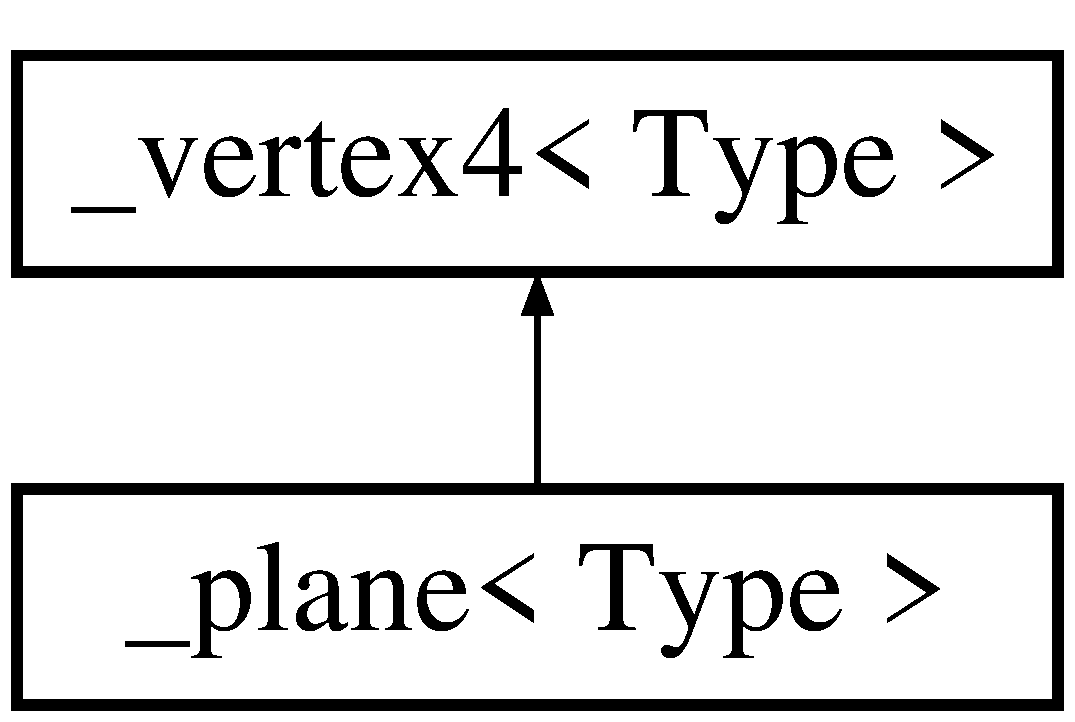
\includegraphics[height=2.000000cm]{class__vertex4}
\end{center}
\end{figure}
\subsection*{Public Member Functions}
\begin{DoxyCompactItemize}
\item 
\hyperlink{class__vertex4_a38ffe3ee599cda54fde6710846c776f9}{\+\_\+vertex4} (Type x1=0, Type y1=0, Type z1=0, Type w1=0)
\item 
\hyperlink{class__vertex4_aad670cc7e7a13a298e8e51cb5b54f26d}{\+\_\+vertex4} (const \hyperlink{class__vertex2}{\+\_\+vertex2}$<$ Type $>$ \&Vertex1)
\item 
\hyperlink{class__vertex4_a1d30459481a974f0231f4a829520acfd}{\+\_\+vertex4} (const \hyperlink{class__vertex3}{\+\_\+vertex3}$<$ Type $>$ \&Vertex1)
\item 
\hyperlink{class__vertex4_ac8132b88505ecf1822c4c88108d221bc}{\+\_\+vertex4} (const \hyperlink{class__vertex4}{\+\_\+vertex4}$<$ Type $>$ \&Vertex1)
\item 
\hyperlink{class__vertex4}{\+\_\+vertex4} \& \hyperlink{class__vertex4_a2794ca2fbcd7994e4b0f98d38c7e5061}{operator()} (Type x1, Type y1, Type z1, Type w1=0)
\item 
\hyperlink{class__vertex4}{\+\_\+vertex4} \& \hyperlink{class__vertex4_a8b7a91ece60ec33e6323652aebc4e055}{operator()} (Type $\ast$Vertices1)
\item 
\hyperlink{class__vertex4}{\+\_\+vertex4} \& \hyperlink{class__vertex4_a025bc24a5016754029ed9161ab08f481}{operator()} (const \hyperlink{class__vertex2}{\+\_\+vertex2}$<$ Type $>$ \&Vertex1)
\item 
\hyperlink{class__vertex4}{\+\_\+vertex4} \& \hyperlink{class__vertex4_a2288c35a419eeecd283c8ec43f2d9c5c}{operator()} (const \hyperlink{class__vertex3}{\+\_\+vertex3}$<$ Type $>$ \&Vertex1)
\item 
\hyperlink{class__vertex4}{\+\_\+vertex4} \& \hyperlink{class__vertex4_a0e077c06875d21b45fcfb2f2f87ab91c}{operator()} (const \hyperlink{class__vertex4}{\+\_\+vertex4}$<$ Type $>$ \&Vertex1)
\item 
\hyperlink{class__vertex4}{\+\_\+vertex4} \& \hyperlink{class__vertex4_ac1708cb9c2a92bfb4984e0230a4e2ac0}{operator=} (const \hyperlink{class__vertex2}{\+\_\+vertex2}$<$ Type $>$ \&Vertex1)
\item 
\hyperlink{class__vertex4}{\+\_\+vertex4} \& \hyperlink{class__vertex4_a0b2cabcff50b85c0f66eb4329bb980a1}{operator=} (const \hyperlink{class__vertex3}{\+\_\+vertex3}$<$ Type $>$ \&Vertex1)
\item 
\hyperlink{class__vertex4}{\+\_\+vertex4} \& \hyperlink{class__vertex4_a270b10fcdaae2eb58adbde6a73b319c7}{operator=} (const \hyperlink{class__vertex4}{\+\_\+vertex4}$<$ Type $>$ \&Vertex1)
\item 
\hyperlink{class__vertex4}{\+\_\+vertex4} \& \hyperlink{class__vertex4_a6280e3485ab56e36668374289b3885e1}{operator=} (Type $\ast$Vertices1)
\item 
\hyperlink{class__vertex4}{\+\_\+vertex4} \hyperlink{class__vertex4_a4eb008aff6cb04a36fc865a51596d7d9}{operator+} (const \hyperlink{class__vertex4}{\+\_\+vertex4}$<$ Type $>$ \&Vertex1)
\item 
\hyperlink{class__vertex4}{\+\_\+vertex4} \& \hyperlink{class__vertex4_adfe5588d11c163da9acbf3872cb44051}{operator+=} (const \hyperlink{class__vertex4}{\+\_\+vertex4}$<$ Type $>$ \&Vertex1)
\item 
\hyperlink{class__vertex4}{\+\_\+vertex4} \hyperlink{class__vertex4_a153c4669c1cd4dc49d6eb6dd7d0a7613}{operator-\/} (const \hyperlink{class__vertex4}{\+\_\+vertex4}$<$ Type $>$ \&Vertex1)
\item 
\hyperlink{class__vertex4}{\+\_\+vertex4} \& \hyperlink{class__vertex4_aa6f0b88ea882bf84362dcc62bc47bdeb}{operator-\/=} (const \hyperlink{class__vertex4}{\+\_\+vertex4}$<$ Type $>$ \&Vertex1)
\item 
\hyperlink{class__vertex4}{\+\_\+vertex4} \hyperlink{class__vertex4_a63177887ce69e51ceaeb6f6649e39374}{operator$\ast$} (Type Value)
\item 
\hyperlink{class__vertex4}{\+\_\+vertex4} \& \hyperlink{class__vertex4_a5a4944a3258f72ac0e23e1e7468bc46e}{operator$\ast$=} (Type Value)
\item 
\hyperlink{class__vertex4}{\+\_\+vertex4} \hyperlink{class__vertex4_a9d5e5beba88204960cd810bc557a74a0}{operator$\ast$} (\hyperlink{class__matrix4}{\+\_\+matrix4}$<$ Type $>$ \&Matrix1)
\item 
\hyperlink{class__vertex4}{\+\_\+vertex4} \& \hyperlink{class__vertex4_aada7301bf2afc5928d3df948201c3ba7}{operator$\ast$=} (\hyperlink{class__matrix4}{\+\_\+matrix4}$<$ Type $>$ \&Matrix1)
\item 
\hyperlink{class__vertex4}{\+\_\+vertex4} \hyperlink{class__vertex4_ab41b97b5865fc9744a28fa359c505a45}{operator/} (Type Value)
\item 
\hyperlink{class__vertex4}{\+\_\+vertex4} \& \hyperlink{class__vertex4_ab4de81fca0447b577dd38dd4b7782994}{operator/=} (Type Value)
\item 
bool \hyperlink{class__vertex4_a1ba75f342bb68a2ce9fe4d8024d6eef7}{operator==} (const \hyperlink{class__vertex4}{\+\_\+vertex4}$<$ Type $>$ \&Vertex1)
\item 
bool \hyperlink{class__vertex4_a0ba4636056d99b8d72e0e1d9f41a0cb6}{operator!=} (const \hyperlink{class__vertex4}{\+\_\+vertex4}$<$ Type $>$ \&Vertex1)
\item 
\hyperlink{class__vertex4}{\+\_\+vertex4} \& \hyperlink{class__vertex4_a3c305186eec5f79b9af562896e79beda}{project} ()
\item 
Type \hyperlink{class__vertex4_ac954b06b01ae8d80b1f33b3a39944026}{dot\+\_\+product} (const \hyperlink{class__vertex4}{\+\_\+vertex4}$<$ Type $>$ \&Vertex1)
\item 
\hyperlink{class__vertex4}{\+\_\+vertex4} \& \hyperlink{class__vertex4_a09ebd88dc99cf80812716f427b104ae6}{normalize} ()
\item 
double \hyperlink{class__vertex4_a91b7559df998c865c54a99cb940d20f9}{module} ()
\item 
\hyperlink{class__vertex4}{\+\_\+vertex4} \hyperlink{class__vertex4_a98da9d52105e5f9660452c653c7b4341}{clone} ()
\item 
Type \& \hyperlink{class__vertex4_acd0acc184dbde695cc2b5505e6b5759e}{operator\mbox{[}$\,$\mbox{]}} (int Position)
\item 
\hyperlink{class__vertex4}{\+\_\+vertex4}$<$ unsigned char $>$ \hyperlink{class__vertex4_a1bfe45c6dd8eedb9699f036e32df3821}{to\+\_\+byte} ()
\item 
\hyperlink{class__vertex4}{\+\_\+vertex4} \& \hyperlink{class__vertex4_a58ed0504721288351f0fc19a23cf2fcc}{from\+\_\+byte} (\hyperlink{class__vertex4}{\+\_\+vertex4}$<$ unsigned char $>$ \&Vertex1)
\item 
void \hyperlink{class__vertex4_ae857f32ed0411c40962cedf68cf7d13e}{show\+\_\+values} ()
\end{DoxyCompactItemize}
\subsection*{Public Attributes}
\begin{DoxyCompactItemize}
\item 
\begin{tabbing}
xx\=xx\=xx\=xx\=xx\=xx\=xx\=xx\=xx\=\kill
union \{\\
\>Type \hyperlink{class__vertex4_a5ccbc85f7d9c91ccbef8b2f43f0f4727}{x}\\
\>Type \hyperlink{class__vertex4_a652faf982e13d7d4ad57c7aa5b933272}{r}\\
\>Type \hyperlink{class__vertex4_aa7123465b4037edc64a3e5d1ee13bfad}{s}\\
\>Type \hyperlink{class__vertex4_a09a23b8ca3bc04a31fcd0ed54b81e0ac}{\_0}\\
\}; \\

\end{tabbing}\item 
\begin{tabbing}
xx\=xx\=xx\=xx\=xx\=xx\=xx\=xx\=xx\=\kill
union \{\\
\>Type \hyperlink{class__vertex4_a8adeda89093117902f2d209dc736e7ea}{y}\\
\>Type \hyperlink{class__vertex4_ab797194de019a14415db3d6c67b53286}{g}\\
\>Type \hyperlink{class__vertex4_a4dd7f37de40f133baaadabda56995781}{t}\\
\>Type \hyperlink{class__vertex4_aaf6e97bf9baa67997950774fab3ed2a3}{\_1}\\
\}; \\

\end{tabbing}\item 
\begin{tabbing}
xx\=xx\=xx\=xx\=xx\=xx\=xx\=xx\=xx\=\kill
union \{\\
\>Type \hyperlink{class__vertex4_afe2944665eb26e649287f8b581c91cc5}{z}\\
\>Type \hyperlink{class__vertex4_ae084625b6693f09ee69fa757251b2f9f}{b}\\
\>Type \hyperlink{class__vertex4_a4cbcf7c136545b28651d1dc5fcd0bcbd}{u}\\
\>Type \hyperlink{class__vertex4_a5023a89cb68c2aa2e43b162d1da600ea}{\_2}\\
\}; \\

\end{tabbing}\item 
\begin{tabbing}
xx\=xx\=xx\=xx\=xx\=xx\=xx\=xx\=xx\=\kill
union \{\\
\>Type \hyperlink{class__vertex4_aedc561486a2aa5aded4b2b931b3aa905}{w}\\
\>Type \hyperlink{class__vertex4_abf7dc914b992f38df50edbcf9e1be42f}{a}\\
\>Type \hyperlink{class__vertex4_aa482b2b78ee03de722c171502ddbff4f}{v}\\
\>Type \hyperlink{class__vertex4_af89b099cc7a2a66fc4db9b3cd5c1dcfb}{\_3}\\
\}; \\

\end{tabbing}\end{DoxyCompactItemize}


\subsection{Constructor \& Destructor Documentation}
\hypertarget{class__vertex4_a38ffe3ee599cda54fde6710846c776f9}{\index{\+\_\+vertex4@{\+\_\+vertex4}!\+\_\+vertex4@{\+\_\+vertex4}}
\index{\+\_\+vertex4@{\+\_\+vertex4}!\+\_\+vertex4@{\+\_\+vertex4}}
\subsubsection[{\+\_\+vertex4}]{\setlength{\rightskip}{0pt plus 5cm}template$<$class Type $>$ {\bf \+\_\+vertex4}$<$ Type $>$\+::{\bf \+\_\+vertex4} (
\begin{DoxyParamCaption}
\item[{Type}]{x1 = {\ttfamily 0}, }
\item[{Type}]{y1 = {\ttfamily 0}, }
\item[{Type}]{z1 = {\ttfamily 0}, }
\item[{Type}]{w1 = {\ttfamily 0}}
\end{DoxyParamCaption}
)}}\label{class__vertex4_a38ffe3ee599cda54fde6710846c776f9}
\hypertarget{class__vertex4_aad670cc7e7a13a298e8e51cb5b54f26d}{\index{\+\_\+vertex4@{\+\_\+vertex4}!\+\_\+vertex4@{\+\_\+vertex4}}
\index{\+\_\+vertex4@{\+\_\+vertex4}!\+\_\+vertex4@{\+\_\+vertex4}}
\subsubsection[{\+\_\+vertex4}]{\setlength{\rightskip}{0pt plus 5cm}template$<$class Type $>$ {\bf \+\_\+vertex4}$<$ Type $>$\+::{\bf \+\_\+vertex4} (
\begin{DoxyParamCaption}
\item[{const {\bf \+\_\+vertex2}$<$ Type $>$ \&}]{Vertex1}
\end{DoxyParamCaption}
)}}\label{class__vertex4_aad670cc7e7a13a298e8e51cb5b54f26d}
\hypertarget{class__vertex4_a1d30459481a974f0231f4a829520acfd}{\index{\+\_\+vertex4@{\+\_\+vertex4}!\+\_\+vertex4@{\+\_\+vertex4}}
\index{\+\_\+vertex4@{\+\_\+vertex4}!\+\_\+vertex4@{\+\_\+vertex4}}
\subsubsection[{\+\_\+vertex4}]{\setlength{\rightskip}{0pt plus 5cm}template$<$class Type $>$ {\bf \+\_\+vertex4}$<$ Type $>$\+::{\bf \+\_\+vertex4} (
\begin{DoxyParamCaption}
\item[{const {\bf \+\_\+vertex3}$<$ Type $>$ \&}]{Vertex1}
\end{DoxyParamCaption}
)}}\label{class__vertex4_a1d30459481a974f0231f4a829520acfd}
\hypertarget{class__vertex4_ac8132b88505ecf1822c4c88108d221bc}{\index{\+\_\+vertex4@{\+\_\+vertex4}!\+\_\+vertex4@{\+\_\+vertex4}}
\index{\+\_\+vertex4@{\+\_\+vertex4}!\+\_\+vertex4@{\+\_\+vertex4}}
\subsubsection[{\+\_\+vertex4}]{\setlength{\rightskip}{0pt plus 5cm}template$<$class Type $>$ {\bf \+\_\+vertex4}$<$ Type $>$\+::{\bf \+\_\+vertex4} (
\begin{DoxyParamCaption}
\item[{const {\bf \+\_\+vertex4}$<$ Type $>$ \&}]{Vertex1}
\end{DoxyParamCaption}
)}}\label{class__vertex4_ac8132b88505ecf1822c4c88108d221bc}


\subsection{Member Function Documentation}
\hypertarget{class__vertex4_a98da9d52105e5f9660452c653c7b4341}{\index{\+\_\+vertex4@{\+\_\+vertex4}!clone@{clone}}
\index{clone@{clone}!\+\_\+vertex4@{\+\_\+vertex4}}
\subsubsection[{clone}]{\setlength{\rightskip}{0pt plus 5cm}template$<$class Type$>$ {\bf \+\_\+vertex4} {\bf \+\_\+vertex4}$<$ Type $>$\+::clone (
\begin{DoxyParamCaption}
{}
\end{DoxyParamCaption}
)\hspace{0.3cm}{\ttfamily [inline]}}}\label{class__vertex4_a98da9d52105e5f9660452c653c7b4341}
\hypertarget{class__vertex4_ac954b06b01ae8d80b1f33b3a39944026}{\index{\+\_\+vertex4@{\+\_\+vertex4}!dot\+\_\+product@{dot\+\_\+product}}
\index{dot\+\_\+product@{dot\+\_\+product}!\+\_\+vertex4@{\+\_\+vertex4}}
\subsubsection[{dot\+\_\+product}]{\setlength{\rightskip}{0pt plus 5cm}template$<$class Type$>$ Type {\bf \+\_\+vertex4}$<$ Type $>$\+::dot\+\_\+product (
\begin{DoxyParamCaption}
\item[{const {\bf \+\_\+vertex4}$<$ Type $>$ \&}]{Vertex1}
\end{DoxyParamCaption}
)\hspace{0.3cm}{\ttfamily [inline]}}}\label{class__vertex4_ac954b06b01ae8d80b1f33b3a39944026}
\hypertarget{class__vertex4_a58ed0504721288351f0fc19a23cf2fcc}{\index{\+\_\+vertex4@{\+\_\+vertex4}!from\+\_\+byte@{from\+\_\+byte}}
\index{from\+\_\+byte@{from\+\_\+byte}!\+\_\+vertex4@{\+\_\+vertex4}}
\subsubsection[{from\+\_\+byte}]{\setlength{\rightskip}{0pt plus 5cm}template$<$class Type $>$ {\bf \+\_\+vertex4}$<$ Type $>$ \& {\bf \+\_\+vertex4}$<$ Type $>$\+::from\+\_\+byte (
\begin{DoxyParamCaption}
\item[{{\bf \+\_\+vertex4}$<$ unsigned char $>$ \&}]{Vertex1}
\end{DoxyParamCaption}
)}}\label{class__vertex4_a58ed0504721288351f0fc19a23cf2fcc}
\hypertarget{class__vertex4_a91b7559df998c865c54a99cb940d20f9}{\index{\+\_\+vertex4@{\+\_\+vertex4}!module@{module}}
\index{module@{module}!\+\_\+vertex4@{\+\_\+vertex4}}
\subsubsection[{module}]{\setlength{\rightskip}{0pt plus 5cm}template$<$class Type$>$ double {\bf \+\_\+vertex4}$<$ Type $>$\+::module (
\begin{DoxyParamCaption}
{}
\end{DoxyParamCaption}
)\hspace{0.3cm}{\ttfamily [inline]}}}\label{class__vertex4_a91b7559df998c865c54a99cb940d20f9}
\hypertarget{class__vertex4_a09ebd88dc99cf80812716f427b104ae6}{\index{\+\_\+vertex4@{\+\_\+vertex4}!normalize@{normalize}}
\index{normalize@{normalize}!\+\_\+vertex4@{\+\_\+vertex4}}
\subsubsection[{normalize}]{\setlength{\rightskip}{0pt plus 5cm}template$<$class Type $>$ {\bf \+\_\+vertex4}$<$ Type $>$ \& {\bf \+\_\+vertex4}$<$ Type $>$\+::normalize (
\begin{DoxyParamCaption}
{}
\end{DoxyParamCaption}
)}}\label{class__vertex4_a09ebd88dc99cf80812716f427b104ae6}
\hypertarget{class__vertex4_a0ba4636056d99b8d72e0e1d9f41a0cb6}{\index{\+\_\+vertex4@{\+\_\+vertex4}!operator"!=@{operator"!=}}
\index{operator"!=@{operator"!=}!\+\_\+vertex4@{\+\_\+vertex4}}
\subsubsection[{operator"!=}]{\setlength{\rightskip}{0pt plus 5cm}template$<$class Type $>$ bool {\bf \+\_\+vertex4}$<$ Type $>$\+::operator!= (
\begin{DoxyParamCaption}
\item[{const {\bf \+\_\+vertex4}$<$ Type $>$ \&}]{Vertex1}
\end{DoxyParamCaption}
)}}\label{class__vertex4_a0ba4636056d99b8d72e0e1d9f41a0cb6}
\hypertarget{class__vertex4_a2794ca2fbcd7994e4b0f98d38c7e5061}{\index{\+\_\+vertex4@{\+\_\+vertex4}!operator()@{operator()}}
\index{operator()@{operator()}!\+\_\+vertex4@{\+\_\+vertex4}}
\subsubsection[{operator()}]{\setlength{\rightskip}{0pt plus 5cm}template$<$class Type $>$ {\bf \+\_\+vertex4}$<$ Type $>$ \& {\bf \+\_\+vertex4}$<$ Type $>$\+::operator() (
\begin{DoxyParamCaption}
\item[{Type}]{x1, }
\item[{Type}]{y1, }
\item[{Type}]{z1, }
\item[{Type}]{w1 = {\ttfamily 0}}
\end{DoxyParamCaption}
)}}\label{class__vertex4_a2794ca2fbcd7994e4b0f98d38c7e5061}
\hypertarget{class__vertex4_a8b7a91ece60ec33e6323652aebc4e055}{\index{\+\_\+vertex4@{\+\_\+vertex4}!operator()@{operator()}}
\index{operator()@{operator()}!\+\_\+vertex4@{\+\_\+vertex4}}
\subsubsection[{operator()}]{\setlength{\rightskip}{0pt plus 5cm}template$<$class Type $>$ {\bf \+\_\+vertex4}$<$ Type $>$ \& {\bf \+\_\+vertex4}$<$ Type $>$\+::operator() (
\begin{DoxyParamCaption}
\item[{Type $\ast$}]{Vertices1}
\end{DoxyParamCaption}
)}}\label{class__vertex4_a8b7a91ece60ec33e6323652aebc4e055}
\hypertarget{class__vertex4_a025bc24a5016754029ed9161ab08f481}{\index{\+\_\+vertex4@{\+\_\+vertex4}!operator()@{operator()}}
\index{operator()@{operator()}!\+\_\+vertex4@{\+\_\+vertex4}}
\subsubsection[{operator()}]{\setlength{\rightskip}{0pt plus 5cm}template$<$class Type $>$ {\bf \+\_\+vertex4}$<$ Type $>$ \& {\bf \+\_\+vertex4}$<$ Type $>$\+::operator() (
\begin{DoxyParamCaption}
\item[{const {\bf \+\_\+vertex2}$<$ Type $>$ \&}]{Vertex1}
\end{DoxyParamCaption}
)}}\label{class__vertex4_a025bc24a5016754029ed9161ab08f481}
\hypertarget{class__vertex4_a2288c35a419eeecd283c8ec43f2d9c5c}{\index{\+\_\+vertex4@{\+\_\+vertex4}!operator()@{operator()}}
\index{operator()@{operator()}!\+\_\+vertex4@{\+\_\+vertex4}}
\subsubsection[{operator()}]{\setlength{\rightskip}{0pt plus 5cm}template$<$class Type $>$ {\bf \+\_\+vertex4}$<$ Type $>$ \& {\bf \+\_\+vertex4}$<$ Type $>$\+::operator() (
\begin{DoxyParamCaption}
\item[{const {\bf \+\_\+vertex3}$<$ Type $>$ \&}]{Vertex1}
\end{DoxyParamCaption}
)}}\label{class__vertex4_a2288c35a419eeecd283c8ec43f2d9c5c}
\hypertarget{class__vertex4_a0e077c06875d21b45fcfb2f2f87ab91c}{\index{\+\_\+vertex4@{\+\_\+vertex4}!operator()@{operator()}}
\index{operator()@{operator()}!\+\_\+vertex4@{\+\_\+vertex4}}
\subsubsection[{operator()}]{\setlength{\rightskip}{0pt plus 5cm}template$<$class Type $>$ {\bf \+\_\+vertex4}$<$ Type $>$ \& {\bf \+\_\+vertex4}$<$ Type $>$\+::operator() (
\begin{DoxyParamCaption}
\item[{const {\bf \+\_\+vertex4}$<$ Type $>$ \&}]{Vertex1}
\end{DoxyParamCaption}
)}}\label{class__vertex4_a0e077c06875d21b45fcfb2f2f87ab91c}
\hypertarget{class__vertex4_a63177887ce69e51ceaeb6f6649e39374}{\index{\+\_\+vertex4@{\+\_\+vertex4}!operator$\ast$@{operator$\ast$}}
\index{operator$\ast$@{operator$\ast$}!\+\_\+vertex4@{\+\_\+vertex4}}
\subsubsection[{operator$\ast$}]{\setlength{\rightskip}{0pt plus 5cm}template$<$class Type $>$ {\bf \+\_\+vertex4}$<$ Type $>$ {\bf \+\_\+vertex4}$<$ Type $>$\+::operator$\ast$ (
\begin{DoxyParamCaption}
\item[{Type}]{Value}
\end{DoxyParamCaption}
)}}\label{class__vertex4_a63177887ce69e51ceaeb6f6649e39374}
\hypertarget{class__vertex4_a9d5e5beba88204960cd810bc557a74a0}{\index{\+\_\+vertex4@{\+\_\+vertex4}!operator$\ast$@{operator$\ast$}}
\index{operator$\ast$@{operator$\ast$}!\+\_\+vertex4@{\+\_\+vertex4}}
\subsubsection[{operator$\ast$}]{\setlength{\rightskip}{0pt plus 5cm}template$<$class Type $>$ {\bf \+\_\+vertex4}$<$ Type $>$ {\bf \+\_\+vertex4}$<$ Type $>$\+::operator$\ast$ (
\begin{DoxyParamCaption}
\item[{{\bf \+\_\+matrix4}$<$ Type $>$ \&}]{Matrix1}
\end{DoxyParamCaption}
)}}\label{class__vertex4_a9d5e5beba88204960cd810bc557a74a0}
\hypertarget{class__vertex4_a5a4944a3258f72ac0e23e1e7468bc46e}{\index{\+\_\+vertex4@{\+\_\+vertex4}!operator$\ast$=@{operator$\ast$=}}
\index{operator$\ast$=@{operator$\ast$=}!\+\_\+vertex4@{\+\_\+vertex4}}
\subsubsection[{operator$\ast$=}]{\setlength{\rightskip}{0pt plus 5cm}template$<$class Type $>$ {\bf \+\_\+vertex4}$<$ Type $>$ \& {\bf \+\_\+vertex4}$<$ Type $>$\+::operator$\ast$= (
\begin{DoxyParamCaption}
\item[{Type}]{Value}
\end{DoxyParamCaption}
)}}\label{class__vertex4_a5a4944a3258f72ac0e23e1e7468bc46e}
\hypertarget{class__vertex4_aada7301bf2afc5928d3df948201c3ba7}{\index{\+\_\+vertex4@{\+\_\+vertex4}!operator$\ast$=@{operator$\ast$=}}
\index{operator$\ast$=@{operator$\ast$=}!\+\_\+vertex4@{\+\_\+vertex4}}
\subsubsection[{operator$\ast$=}]{\setlength{\rightskip}{0pt plus 5cm}template$<$class Type $>$ {\bf \+\_\+vertex4}$<$ Type $>$ \& {\bf \+\_\+vertex4}$<$ Type $>$\+::operator$\ast$= (
\begin{DoxyParamCaption}
\item[{{\bf \+\_\+matrix4}$<$ Type $>$ \&}]{Matrix1}
\end{DoxyParamCaption}
)}}\label{class__vertex4_aada7301bf2afc5928d3df948201c3ba7}
\hypertarget{class__vertex4_a4eb008aff6cb04a36fc865a51596d7d9}{\index{\+\_\+vertex4@{\+\_\+vertex4}!operator+@{operator+}}
\index{operator+@{operator+}!\+\_\+vertex4@{\+\_\+vertex4}}
\subsubsection[{operator+}]{\setlength{\rightskip}{0pt plus 5cm}template$<$class Type $>$ {\bf \+\_\+vertex4}$<$ Type $>$ {\bf \+\_\+vertex4}$<$ Type $>$\+::operator+ (
\begin{DoxyParamCaption}
\item[{const {\bf \+\_\+vertex4}$<$ Type $>$ \&}]{Vertex1}
\end{DoxyParamCaption}
)}}\label{class__vertex4_a4eb008aff6cb04a36fc865a51596d7d9}
\hypertarget{class__vertex4_adfe5588d11c163da9acbf3872cb44051}{\index{\+\_\+vertex4@{\+\_\+vertex4}!operator+=@{operator+=}}
\index{operator+=@{operator+=}!\+\_\+vertex4@{\+\_\+vertex4}}
\subsubsection[{operator+=}]{\setlength{\rightskip}{0pt plus 5cm}template$<$class Type $>$ {\bf \+\_\+vertex4}$<$ Type $>$ \& {\bf \+\_\+vertex4}$<$ Type $>$\+::operator+= (
\begin{DoxyParamCaption}
\item[{const {\bf \+\_\+vertex4}$<$ Type $>$ \&}]{Vertex1}
\end{DoxyParamCaption}
)}}\label{class__vertex4_adfe5588d11c163da9acbf3872cb44051}
\hypertarget{class__vertex4_a153c4669c1cd4dc49d6eb6dd7d0a7613}{\index{\+\_\+vertex4@{\+\_\+vertex4}!operator-\/@{operator-\/}}
\index{operator-\/@{operator-\/}!\+\_\+vertex4@{\+\_\+vertex4}}
\subsubsection[{operator-\/}]{\setlength{\rightskip}{0pt plus 5cm}template$<$class Type $>$ {\bf \+\_\+vertex4}$<$ Type $>$ {\bf \+\_\+vertex4}$<$ Type $>$\+::operator-\/ (
\begin{DoxyParamCaption}
\item[{const {\bf \+\_\+vertex4}$<$ Type $>$ \&}]{Vertex1}
\end{DoxyParamCaption}
)}}\label{class__vertex4_a153c4669c1cd4dc49d6eb6dd7d0a7613}
\hypertarget{class__vertex4_aa6f0b88ea882bf84362dcc62bc47bdeb}{\index{\+\_\+vertex4@{\+\_\+vertex4}!operator-\/=@{operator-\/=}}
\index{operator-\/=@{operator-\/=}!\+\_\+vertex4@{\+\_\+vertex4}}
\subsubsection[{operator-\/=}]{\setlength{\rightskip}{0pt plus 5cm}template$<$class Type $>$ {\bf \+\_\+vertex4}$<$ Type $>$ \& {\bf \+\_\+vertex4}$<$ Type $>$\+::operator-\/= (
\begin{DoxyParamCaption}
\item[{const {\bf \+\_\+vertex4}$<$ Type $>$ \&}]{Vertex1}
\end{DoxyParamCaption}
)}}\label{class__vertex4_aa6f0b88ea882bf84362dcc62bc47bdeb}
\hypertarget{class__vertex4_ab41b97b5865fc9744a28fa359c505a45}{\index{\+\_\+vertex4@{\+\_\+vertex4}!operator/@{operator/}}
\index{operator/@{operator/}!\+\_\+vertex4@{\+\_\+vertex4}}
\subsubsection[{operator/}]{\setlength{\rightskip}{0pt plus 5cm}template$<$class Type $>$ {\bf \+\_\+vertex4}$<$ Type $>$ {\bf \+\_\+vertex4}$<$ Type $>$\+::operator/ (
\begin{DoxyParamCaption}
\item[{Type}]{Value}
\end{DoxyParamCaption}
)}}\label{class__vertex4_ab41b97b5865fc9744a28fa359c505a45}
\hypertarget{class__vertex4_ab4de81fca0447b577dd38dd4b7782994}{\index{\+\_\+vertex4@{\+\_\+vertex4}!operator/=@{operator/=}}
\index{operator/=@{operator/=}!\+\_\+vertex4@{\+\_\+vertex4}}
\subsubsection[{operator/=}]{\setlength{\rightskip}{0pt plus 5cm}template$<$class Type $>$ {\bf \+\_\+vertex4}$<$ Type $>$ \& {\bf \+\_\+vertex4}$<$ Type $>$\+::operator/= (
\begin{DoxyParamCaption}
\item[{Type}]{Value}
\end{DoxyParamCaption}
)}}\label{class__vertex4_ab4de81fca0447b577dd38dd4b7782994}
\hypertarget{class__vertex4_ac1708cb9c2a92bfb4984e0230a4e2ac0}{\index{\+\_\+vertex4@{\+\_\+vertex4}!operator=@{operator=}}
\index{operator=@{operator=}!\+\_\+vertex4@{\+\_\+vertex4}}
\subsubsection[{operator=}]{\setlength{\rightskip}{0pt plus 5cm}template$<$class Type $>$ {\bf \+\_\+vertex4}$<$ Type $>$ \& {\bf \+\_\+vertex4}$<$ Type $>$\+::operator= (
\begin{DoxyParamCaption}
\item[{const {\bf \+\_\+vertex2}$<$ Type $>$ \&}]{Vertex1}
\end{DoxyParamCaption}
)}}\label{class__vertex4_ac1708cb9c2a92bfb4984e0230a4e2ac0}
\hypertarget{class__vertex4_a0b2cabcff50b85c0f66eb4329bb980a1}{\index{\+\_\+vertex4@{\+\_\+vertex4}!operator=@{operator=}}
\index{operator=@{operator=}!\+\_\+vertex4@{\+\_\+vertex4}}
\subsubsection[{operator=}]{\setlength{\rightskip}{0pt plus 5cm}template$<$class Type $>$ {\bf \+\_\+vertex4}$<$ Type $>$ \& {\bf \+\_\+vertex4}$<$ Type $>$\+::operator= (
\begin{DoxyParamCaption}
\item[{const {\bf \+\_\+vertex3}$<$ Type $>$ \&}]{Vertex1}
\end{DoxyParamCaption}
)}}\label{class__vertex4_a0b2cabcff50b85c0f66eb4329bb980a1}
\hypertarget{class__vertex4_a270b10fcdaae2eb58adbde6a73b319c7}{\index{\+\_\+vertex4@{\+\_\+vertex4}!operator=@{operator=}}
\index{operator=@{operator=}!\+\_\+vertex4@{\+\_\+vertex4}}
\subsubsection[{operator=}]{\setlength{\rightskip}{0pt plus 5cm}template$<$class Type $>$ {\bf \+\_\+vertex4}$<$ Type $>$ \& {\bf \+\_\+vertex4}$<$ Type $>$\+::operator= (
\begin{DoxyParamCaption}
\item[{const {\bf \+\_\+vertex4}$<$ Type $>$ \&}]{Vertex1}
\end{DoxyParamCaption}
)}}\label{class__vertex4_a270b10fcdaae2eb58adbde6a73b319c7}
\hypertarget{class__vertex4_a6280e3485ab56e36668374289b3885e1}{\index{\+\_\+vertex4@{\+\_\+vertex4}!operator=@{operator=}}
\index{operator=@{operator=}!\+\_\+vertex4@{\+\_\+vertex4}}
\subsubsection[{operator=}]{\setlength{\rightskip}{0pt plus 5cm}template$<$class Type $>$ {\bf \+\_\+vertex4}$<$ Type $>$ \& {\bf \+\_\+vertex4}$<$ Type $>$\+::operator= (
\begin{DoxyParamCaption}
\item[{Type $\ast$}]{Vertices1}
\end{DoxyParamCaption}
)}}\label{class__vertex4_a6280e3485ab56e36668374289b3885e1}
\hypertarget{class__vertex4_a1ba75f342bb68a2ce9fe4d8024d6eef7}{\index{\+\_\+vertex4@{\+\_\+vertex4}!operator==@{operator==}}
\index{operator==@{operator==}!\+\_\+vertex4@{\+\_\+vertex4}}
\subsubsection[{operator==}]{\setlength{\rightskip}{0pt plus 5cm}template$<$class Type $>$ bool {\bf \+\_\+vertex4}$<$ Type $>$\+::operator== (
\begin{DoxyParamCaption}
\item[{const {\bf \+\_\+vertex4}$<$ Type $>$ \&}]{Vertex1}
\end{DoxyParamCaption}
)}}\label{class__vertex4_a1ba75f342bb68a2ce9fe4d8024d6eef7}
\hypertarget{class__vertex4_acd0acc184dbde695cc2b5505e6b5759e}{\index{\+\_\+vertex4@{\+\_\+vertex4}!operator\mbox{[}$\,$\mbox{]}@{operator[]}}
\index{operator\mbox{[}$\,$\mbox{]}@{operator[]}!\+\_\+vertex4@{\+\_\+vertex4}}
\subsubsection[{operator[]}]{\setlength{\rightskip}{0pt plus 5cm}template$<$class Type$>$ Type\& {\bf \+\_\+vertex4}$<$ Type $>$\+::operator\mbox{[}$\,$\mbox{]} (
\begin{DoxyParamCaption}
\item[{int}]{Position}
\end{DoxyParamCaption}
)\hspace{0.3cm}{\ttfamily [inline]}}}\label{class__vertex4_acd0acc184dbde695cc2b5505e6b5759e}
\hypertarget{class__vertex4_a3c305186eec5f79b9af562896e79beda}{\index{\+\_\+vertex4@{\+\_\+vertex4}!project@{project}}
\index{project@{project}!\+\_\+vertex4@{\+\_\+vertex4}}
\subsubsection[{project}]{\setlength{\rightskip}{0pt plus 5cm}template$<$class Type $>$ {\bf \+\_\+vertex4}$<$ Type $>$ \& {\bf \+\_\+vertex4}$<$ Type $>$\+::project (
\begin{DoxyParamCaption}
{}
\end{DoxyParamCaption}
)}}\label{class__vertex4_a3c305186eec5f79b9af562896e79beda}
\hypertarget{class__vertex4_ae857f32ed0411c40962cedf68cf7d13e}{\index{\+\_\+vertex4@{\+\_\+vertex4}!show\+\_\+values@{show\+\_\+values}}
\index{show\+\_\+values@{show\+\_\+values}!\+\_\+vertex4@{\+\_\+vertex4}}
\subsubsection[{show\+\_\+values}]{\setlength{\rightskip}{0pt plus 5cm}template$<$class Type $>$ void {\bf \+\_\+vertex4}$<$ Type $>$\+::show\+\_\+values (
\begin{DoxyParamCaption}
{}
\end{DoxyParamCaption}
)}}\label{class__vertex4_ae857f32ed0411c40962cedf68cf7d13e}
\hypertarget{class__vertex4_a1bfe45c6dd8eedb9699f036e32df3821}{\index{\+\_\+vertex4@{\+\_\+vertex4}!to\+\_\+byte@{to\+\_\+byte}}
\index{to\+\_\+byte@{to\+\_\+byte}!\+\_\+vertex4@{\+\_\+vertex4}}
\subsubsection[{to\+\_\+byte}]{\setlength{\rightskip}{0pt plus 5cm}template$<$class Type $>$ {\bf \+\_\+vertex4}$<$ unsigned char $>$ {\bf \+\_\+vertex4}$<$ Type $>$\+::to\+\_\+byte (
\begin{DoxyParamCaption}
{}
\end{DoxyParamCaption}
)}}\label{class__vertex4_a1bfe45c6dd8eedb9699f036e32df3821}


\subsection{Member Data Documentation}
\hypertarget{class__vertex4_ace50a28d1947b55e8320c2d6d9357a53}{\subsubsection[{"@11}]{\setlength{\rightskip}{0pt plus 5cm}union \{ ... \} }}\label{class__vertex4_ace50a28d1947b55e8320c2d6d9357a53}
\hypertarget{class__vertex4_a58573aec2b21f5f8847f249b08ed1a06}{\subsubsection[{"@13}]{\setlength{\rightskip}{0pt plus 5cm}union \{ ... \} }}\label{class__vertex4_a58573aec2b21f5f8847f249b08ed1a06}
\hypertarget{class__vertex4_a937d6b630a10567e28fc9a908153cfbf}{\subsubsection[{"@15}]{\setlength{\rightskip}{0pt plus 5cm}union \{ ... \} }}\label{class__vertex4_a937d6b630a10567e28fc9a908153cfbf}
\hypertarget{class__vertex4_a327f4644f527b94b21efac763ff56515}{\subsubsection[{"@17}]{\setlength{\rightskip}{0pt plus 5cm}union \{ ... \} }}\label{class__vertex4_a327f4644f527b94b21efac763ff56515}
\hypertarget{class__vertex4_a09a23b8ca3bc04a31fcd0ed54b81e0ac}{\index{\+\_\+vertex4@{\+\_\+vertex4}!\+\_\+0@{\+\_\+0}}
\index{\+\_\+0@{\+\_\+0}!\+\_\+vertex4@{\+\_\+vertex4}}
\subsubsection[{\+\_\+0}]{\setlength{\rightskip}{0pt plus 5cm}template$<$class Type$>$ Type {\bf \+\_\+vertex4}$<$ Type $>$\+::\+\_\+0}}\label{class__vertex4_a09a23b8ca3bc04a31fcd0ed54b81e0ac}
\hypertarget{class__vertex4_aaf6e97bf9baa67997950774fab3ed2a3}{\index{\+\_\+vertex4@{\+\_\+vertex4}!\+\_\+1@{\+\_\+1}}
\index{\+\_\+1@{\+\_\+1}!\+\_\+vertex4@{\+\_\+vertex4}}
\subsubsection[{\+\_\+1}]{\setlength{\rightskip}{0pt plus 5cm}template$<$class Type$>$ Type {\bf \+\_\+vertex4}$<$ Type $>$\+::\+\_\+1}}\label{class__vertex4_aaf6e97bf9baa67997950774fab3ed2a3}
\hypertarget{class__vertex4_a5023a89cb68c2aa2e43b162d1da600ea}{\index{\+\_\+vertex4@{\+\_\+vertex4}!\+\_\+2@{\+\_\+2}}
\index{\+\_\+2@{\+\_\+2}!\+\_\+vertex4@{\+\_\+vertex4}}
\subsubsection[{\+\_\+2}]{\setlength{\rightskip}{0pt plus 5cm}template$<$class Type$>$ Type {\bf \+\_\+vertex4}$<$ Type $>$\+::\+\_\+2}}\label{class__vertex4_a5023a89cb68c2aa2e43b162d1da600ea}
\hypertarget{class__vertex4_af89b099cc7a2a66fc4db9b3cd5c1dcfb}{\index{\+\_\+vertex4@{\+\_\+vertex4}!\+\_\+3@{\+\_\+3}}
\index{\+\_\+3@{\+\_\+3}!\+\_\+vertex4@{\+\_\+vertex4}}
\subsubsection[{\+\_\+3}]{\setlength{\rightskip}{0pt plus 5cm}template$<$class Type$>$ Type {\bf \+\_\+vertex4}$<$ Type $>$\+::\+\_\+3}}\label{class__vertex4_af89b099cc7a2a66fc4db9b3cd5c1dcfb}
\hypertarget{class__vertex4_abf7dc914b992f38df50edbcf9e1be42f}{\index{\+\_\+vertex4@{\+\_\+vertex4}!a@{a}}
\index{a@{a}!\+\_\+vertex4@{\+\_\+vertex4}}
\subsubsection[{a}]{\setlength{\rightskip}{0pt plus 5cm}template$<$class Type$>$ Type {\bf \+\_\+vertex4}$<$ Type $>$\+::a}}\label{class__vertex4_abf7dc914b992f38df50edbcf9e1be42f}
\hypertarget{class__vertex4_ae084625b6693f09ee69fa757251b2f9f}{\index{\+\_\+vertex4@{\+\_\+vertex4}!b@{b}}
\index{b@{b}!\+\_\+vertex4@{\+\_\+vertex4}}
\subsubsection[{b}]{\setlength{\rightskip}{0pt plus 5cm}template$<$class Type$>$ Type {\bf \+\_\+vertex4}$<$ Type $>$\+::b}}\label{class__vertex4_ae084625b6693f09ee69fa757251b2f9f}
\hypertarget{class__vertex4_ab797194de019a14415db3d6c67b53286}{\index{\+\_\+vertex4@{\+\_\+vertex4}!g@{g}}
\index{g@{g}!\+\_\+vertex4@{\+\_\+vertex4}}
\subsubsection[{g}]{\setlength{\rightskip}{0pt plus 5cm}template$<$class Type$>$ Type {\bf \+\_\+vertex4}$<$ Type $>$\+::g}}\label{class__vertex4_ab797194de019a14415db3d6c67b53286}
\hypertarget{class__vertex4_a652faf982e13d7d4ad57c7aa5b933272}{\index{\+\_\+vertex4@{\+\_\+vertex4}!r@{r}}
\index{r@{r}!\+\_\+vertex4@{\+\_\+vertex4}}
\subsubsection[{r}]{\setlength{\rightskip}{0pt plus 5cm}template$<$class Type$>$ Type {\bf \+\_\+vertex4}$<$ Type $>$\+::r}}\label{class__vertex4_a652faf982e13d7d4ad57c7aa5b933272}
\hypertarget{class__vertex4_aa7123465b4037edc64a3e5d1ee13bfad}{\index{\+\_\+vertex4@{\+\_\+vertex4}!s@{s}}
\index{s@{s}!\+\_\+vertex4@{\+\_\+vertex4}}
\subsubsection[{s}]{\setlength{\rightskip}{0pt plus 5cm}template$<$class Type$>$ Type {\bf \+\_\+vertex4}$<$ Type $>$\+::s}}\label{class__vertex4_aa7123465b4037edc64a3e5d1ee13bfad}
\hypertarget{class__vertex4_a4dd7f37de40f133baaadabda56995781}{\index{\+\_\+vertex4@{\+\_\+vertex4}!t@{t}}
\index{t@{t}!\+\_\+vertex4@{\+\_\+vertex4}}
\subsubsection[{t}]{\setlength{\rightskip}{0pt plus 5cm}template$<$class Type$>$ Type {\bf \+\_\+vertex4}$<$ Type $>$\+::t}}\label{class__vertex4_a4dd7f37de40f133baaadabda56995781}
\hypertarget{class__vertex4_a4cbcf7c136545b28651d1dc5fcd0bcbd}{\index{\+\_\+vertex4@{\+\_\+vertex4}!u@{u}}
\index{u@{u}!\+\_\+vertex4@{\+\_\+vertex4}}
\subsubsection[{u}]{\setlength{\rightskip}{0pt plus 5cm}template$<$class Type$>$ Type {\bf \+\_\+vertex4}$<$ Type $>$\+::u}}\label{class__vertex4_a4cbcf7c136545b28651d1dc5fcd0bcbd}
\hypertarget{class__vertex4_aa482b2b78ee03de722c171502ddbff4f}{\index{\+\_\+vertex4@{\+\_\+vertex4}!v@{v}}
\index{v@{v}!\+\_\+vertex4@{\+\_\+vertex4}}
\subsubsection[{v}]{\setlength{\rightskip}{0pt plus 5cm}template$<$class Type$>$ Type {\bf \+\_\+vertex4}$<$ Type $>$\+::v}}\label{class__vertex4_aa482b2b78ee03de722c171502ddbff4f}
\hypertarget{class__vertex4_aedc561486a2aa5aded4b2b931b3aa905}{\index{\+\_\+vertex4@{\+\_\+vertex4}!w@{w}}
\index{w@{w}!\+\_\+vertex4@{\+\_\+vertex4}}
\subsubsection[{w}]{\setlength{\rightskip}{0pt plus 5cm}template$<$class Type$>$ Type {\bf \+\_\+vertex4}$<$ Type $>$\+::w}}\label{class__vertex4_aedc561486a2aa5aded4b2b931b3aa905}
\hypertarget{class__vertex4_a5ccbc85f7d9c91ccbef8b2f43f0f4727}{\index{\+\_\+vertex4@{\+\_\+vertex4}!x@{x}}
\index{x@{x}!\+\_\+vertex4@{\+\_\+vertex4}}
\subsubsection[{x}]{\setlength{\rightskip}{0pt plus 5cm}template$<$class Type$>$ Type {\bf \+\_\+vertex4}$<$ Type $>$\+::x}}\label{class__vertex4_a5ccbc85f7d9c91ccbef8b2f43f0f4727}
\hypertarget{class__vertex4_a8adeda89093117902f2d209dc736e7ea}{\index{\+\_\+vertex4@{\+\_\+vertex4}!y@{y}}
\index{y@{y}!\+\_\+vertex4@{\+\_\+vertex4}}
\subsubsection[{y}]{\setlength{\rightskip}{0pt plus 5cm}template$<$class Type$>$ Type {\bf \+\_\+vertex4}$<$ Type $>$\+::y}}\label{class__vertex4_a8adeda89093117902f2d209dc736e7ea}
\hypertarget{class__vertex4_afe2944665eb26e649287f8b581c91cc5}{\index{\+\_\+vertex4@{\+\_\+vertex4}!z@{z}}
\index{z@{z}!\+\_\+vertex4@{\+\_\+vertex4}}
\subsubsection[{z}]{\setlength{\rightskip}{0pt plus 5cm}template$<$class Type$>$ Type {\bf \+\_\+vertex4}$<$ Type $>$\+::z}}\label{class__vertex4_afe2944665eb26e649287f8b581c91cc5}


The documentation for this class was generated from the following file\+:\begin{DoxyCompactItemize}
\item 
\hyperlink{vertex_8h}{vertex.\+h}\end{DoxyCompactItemize}

\chapter{File Documentation}
\hypertarget{file__ply__stl_8cc}{\section{file\+\_\+ply\+\_\+stl.\+cc File Reference}
\label{file__ply__stl_8cc}\index{file\+\_\+ply\+\_\+stl.\+cc@{file\+\_\+ply\+\_\+stl.\+cc}}
}
{\ttfamily \#include \char`\"{}file\+\_\+ply\+\_\+stl.\+hpp\char`\"{}}\\*
\subsection*{Namespaces}
\begin{DoxyCompactItemize}
\item 
 \hyperlink{namespace__file__ply}{\+\_\+file\+\_\+ply}
\end{DoxyCompactItemize}
\subsection*{Functions}
\begin{DoxyCompactItemize}
\item 
void \hyperlink{namespace__file__ply_a1da8b0ac0e1febd8984cfbf7b9f3c682}{\+\_\+file\+\_\+ply\+::error} (const char $\ast$msg\+Error)
\item 
void \hyperlink{namespace__file__ply_a4958ec9c225bd88927de9ba6115810a9}{\+\_\+file\+\_\+ply\+::read} (const char $\ast$nombre\+Archivo, vector$<$ double $>$ \&vertices, vector$<$ unsigned long $>$ \&faces)
\end{DoxyCompactItemize}
\subsection*{Variables}
\begin{DoxyCompactItemize}
\item 
const streamsize \hyperlink{namespace__file__ply_a66e58e4b840d28ffd29b2d78360cc365}{\+\_\+file\+\_\+ply\+::buffer\+Capacity} = streamsize(10)$\ast$streamsize(1024)
\item 
char \hyperlink{namespace__file__ply_a0f387576a0c9b81853271b839973e850}{\+\_\+file\+\_\+ply\+::buffer} \mbox{[}(unsigned long)(buffer\+Capacity)\mbox{]}
\end{DoxyCompactItemize}

\hypertarget{file__ply__stl_8hpp}{\section{file\+\_\+ply\+\_\+stl.\+hpp File Reference}
\label{file__ply__stl_8hpp}\index{file\+\_\+ply\+\_\+stl.\+hpp@{file\+\_\+ply\+\_\+stl.\+hpp}}
}
{\ttfamily \#include $<$stdio.\+h$>$}\\*
{\ttfamily \#include $<$stdlib.\+h$>$}\\*
{\ttfamily \#include $<$string.\+h$>$}\\*
{\ttfamily \#include $<$string$>$}\\*
{\ttfamily \#include $<$vector$>$}\\*
{\ttfamily \#include $<$iostream$>$}\\*
{\ttfamily \#include $<$fstream$>$}\\*
{\ttfamily \#include $<$cmath$>$}\\*
{\ttfamily \#include $<$assert.\+h$>$}\\*
\subsection*{Namespaces}
\begin{DoxyCompactItemize}
\item 
 \hyperlink{namespace__file__ply}{\+\_\+file\+\_\+ply}
\end{DoxyCompactItemize}
\subsection*{Functions}
\begin{DoxyCompactItemize}
\item 
void \hyperlink{namespace__file__ply_a4958ec9c225bd88927de9ba6115810a9}{\+\_\+file\+\_\+ply\+::read} (const char $\ast$nombre\+Archivo, vector$<$ double $>$ \&vertices, vector$<$ unsigned long $>$ \&faces)
\end{DoxyCompactItemize}

\hypertarget{main_8cc}{\section{main.\+cc File Reference}
\label{main_8cc}\index{main.\+cc@{main.\+cc}}
}
{\ttfamily \#include \char`\"{}stdlib.\+h\char`\"{}}\\*
{\ttfamily \#include \char`\"{}stdio.\+h\char`\"{}}\\*
{\ttfamily \#include $<$windows.\+h$>$}\\*
{\ttfamily \#include $<$G\+L/glut.\+h$>$}\\*
{\ttfamily \#include $<$ctype.\+h$>$}\\*
{\ttfamily \#include \char`\"{}user\+\_\+code.\+h\char`\"{}}\\*
{\ttfamily \#include $<$iostream$>$}\\*
{\ttfamily \#include \char`\"{}file\+\_\+ply\+\_\+stl.\+hpp\char`\"{}}\\*
\subsection*{Functions}
\begin{DoxyCompactItemize}
\item 
void \hyperlink{main_8cc_a9b7ad4d65a150223cf538ab8dd6317bd}{clear\+\_\+window} ()
\item 
void \hyperlink{main_8cc_af9b396b692aa46ba7ffd48d28f1905ab}{change\+\_\+projection} ()
\item 
void \hyperlink{main_8cc_aac0de658d992bdff01a8cc06065c1bcd}{change\+\_\+observer} ()
\item 
void \hyperlink{main_8cc_a0a236f4909cc881ca1413b078b6631bd}{draw\+\_\+axis} ()
\item 
void \hyperlink{main_8cc_a510234391685c122fc0e1daf817f415d}{draw\+\_\+objects} ()
\item 
void \hyperlink{main_8cc_a64dd25fa03ac084b0cd583c633f49e53}{draw\+\_\+scene} (void)
\item 
void \hyperlink{main_8cc_ad5415072496ea3d9373acf0dc16451ea}{change\+\_\+window\+\_\+size} (int Ancho1, int Alto1)
\item 
void \hyperlink{main_8cc_ae37929ade04a55bb53bd366fd188f944}{normal\+\_\+keys} (unsigned char Tecla1, int x, int y)
\item 
void \hyperlink{main_8cc_ac82294b959edb3284999c0f4449b8cbd}{special\+\_\+keys} (int Tecla1, int x, int y)
\item 
void \hyperlink{main_8cc_a9efe22aaead3a5e936b5df459de02eba}{initialize} (void)
\item 
int \hyperlink{main_8cc_a3c04138a5bfe5d72780bb7e82a18e627}{main} (int argc, char $\ast$$\ast$argv)
\end{DoxyCompactItemize}
\subsection*{Variables}
\begin{DoxyCompactItemize}
\item 
const int \hyperlink{main_8cc_a9255790b9394e098f4a3bb020b763825}{A\+X\+I\+S\+\_\+\+S\+I\+Z\+E} =5000
\begin{DoxyCompactList}\small\item\em Tamaño de los ejes. \end{DoxyCompactList}\item 
G\+Lfloat \hyperlink{main_8cc_a62d6a08bb1b879dcb733ee7c12d7eba0}{Observer\+\_\+distance}
\begin{DoxyCompactList}\small\item\em variables que definen la posicion de la camara en coordenadas polares \end{DoxyCompactList}\item 
G\+Lfloat \hyperlink{main_8cc_a9ad7aa10ae4b96ee8e0d0befc46e0342}{Observer\+\_\+angle\+\_\+x}
\item 
G\+Lfloat \hyperlink{main_8cc_a92a40873062a6bf329781179e96ea076}{Observer\+\_\+angle\+\_\+y}
\item 
int \hyperlink{main_8cc_a80a769ffbed195e9646be97726d7fac7}{E\+S\+T\+I\+L\+O} =0
\item 
int \hyperlink{main_8cc_a9cd2c9e18d1943e83493edf94302db5b}{F\+I\+C\+H\+E\+R\+O} =0
\item 
bool \hyperlink{main_8cc_abd34ae937ae90265d7aa9feac401b069}{M\+I\+T\+A\+D} =false
\item 
int \hyperlink{main_8cc_ac75ef3236eddefc656815d243bd0f215}{E\+S\+P\+E\+C\+I\+A\+L} =0
\item 
int \hyperlink{main_8cc_a227bf92957b72bf606d7e059f510c6ec}{E\+S\+P\+E\+C\+I\+A\+L2} =0
\item 
G\+Lfloat \hyperlink{main_8cc_a9a6d5bceee8b5603001327ee69f29b1f}{Window\+\_\+width}
\item 
G\+Lfloat \hyperlink{main_8cc_a21be4d123a277604058424c46e1d3a0c}{Window\+\_\+height}
\item 
G\+Lfloat \hyperlink{main_8cc_ac566cb0ef197ee9f242138983f0e9bac}{Front\+\_\+plane}
\item 
G\+Lfloat \hyperlink{main_8cc_ac2f441805017f335408f7f734dfc5429}{Back\+\_\+plane}
\item 
int \hyperlink{main_8cc_a976847963dc730d99e17f4fec10652f3}{U\+I\+\_\+window\+\_\+pos\+\_\+x} =50
\item 
int \hyperlink{main_8cc_a8c0a4be10a8bd129c871cea302eed924}{U\+I\+\_\+window\+\_\+pos\+\_\+y} =50
\item 
int \hyperlink{main_8cc_a92e9f5bc39c5f59b3a740a4d67babb8b}{U\+I\+\_\+window\+\_\+width} =500
\item 
int \hyperlink{main_8cc_a83c72fa8e1f0b764f1014644eaa5561e}{U\+I\+\_\+window\+\_\+height} =500
\end{DoxyCompactItemize}


\subsection{Function Documentation}
\hypertarget{main_8cc_aac0de658d992bdff01a8cc06065c1bcd}{\index{main.\+cc@{main.\+cc}!change\+\_\+observer@{change\+\_\+observer}}
\index{change\+\_\+observer@{change\+\_\+observer}!main.\+cc@{main.\+cc}}
\subsubsection[{change\+\_\+observer}]{\setlength{\rightskip}{0pt plus 5cm}void change\+\_\+observer (
\begin{DoxyParamCaption}
{}
\end{DoxyParamCaption}
)}}\label{main_8cc_aac0de658d992bdff01a8cc06065c1bcd}
\hypertarget{main_8cc_af9b396b692aa46ba7ffd48d28f1905ab}{\index{main.\+cc@{main.\+cc}!change\+\_\+projection@{change\+\_\+projection}}
\index{change\+\_\+projection@{change\+\_\+projection}!main.\+cc@{main.\+cc}}
\subsubsection[{change\+\_\+projection}]{\setlength{\rightskip}{0pt plus 5cm}void change\+\_\+projection (
\begin{DoxyParamCaption}
{}
\end{DoxyParamCaption}
)}}\label{main_8cc_af9b396b692aa46ba7ffd48d28f1905ab}
\hypertarget{main_8cc_ad5415072496ea3d9373acf0dc16451ea}{\index{main.\+cc@{main.\+cc}!change\+\_\+window\+\_\+size@{change\+\_\+window\+\_\+size}}
\index{change\+\_\+window\+\_\+size@{change\+\_\+window\+\_\+size}!main.\+cc@{main.\+cc}}
\subsubsection[{change\+\_\+window\+\_\+size}]{\setlength{\rightskip}{0pt plus 5cm}void change\+\_\+window\+\_\+size (
\begin{DoxyParamCaption}
\item[{int}]{Ancho1, }
\item[{int}]{Alto1}
\end{DoxyParamCaption}
)}}\label{main_8cc_ad5415072496ea3d9373acf0dc16451ea}
Funcion llamada cuando se produce un cambio en el tamaño de la ventana el evento manda a la funcion\+: nuevo ancho nuevo alto \hypertarget{main_8cc_a9b7ad4d65a150223cf538ab8dd6317bd}{\index{main.\+cc@{main.\+cc}!clear\+\_\+window@{clear\+\_\+window}}
\index{clear\+\_\+window@{clear\+\_\+window}!main.\+cc@{main.\+cc}}
\subsubsection[{clear\+\_\+window}]{\setlength{\rightskip}{0pt plus 5cm}void clear\+\_\+window (
\begin{DoxyParamCaption}
{}
\end{DoxyParamCaption}
)}}\label{main_8cc_a9b7ad4d65a150223cf538ab8dd6317bd}
\hypertarget{main_8cc_a0a236f4909cc881ca1413b078b6631bd}{\index{main.\+cc@{main.\+cc}!draw\+\_\+axis@{draw\+\_\+axis}}
\index{draw\+\_\+axis@{draw\+\_\+axis}!main.\+cc@{main.\+cc}}
\subsubsection[{draw\+\_\+axis}]{\setlength{\rightskip}{0pt plus 5cm}void draw\+\_\+axis (
\begin{DoxyParamCaption}
{}
\end{DoxyParamCaption}
)}}\label{main_8cc_a0a236f4909cc881ca1413b078b6631bd}
\hypertarget{main_8cc_a510234391685c122fc0e1daf817f415d}{\index{main.\+cc@{main.\+cc}!draw\+\_\+objects@{draw\+\_\+objects}}
\index{draw\+\_\+objects@{draw\+\_\+objects}!main.\+cc@{main.\+cc}}
\subsubsection[{draw\+\_\+objects}]{\setlength{\rightskip}{0pt plus 5cm}void draw\+\_\+objects (
\begin{DoxyParamCaption}
{}
\end{DoxyParamCaption}
)}}\label{main_8cc_a510234391685c122fc0e1daf817f415d}
\hypertarget{main_8cc_a64dd25fa03ac084b0cd583c633f49e53}{\index{main.\+cc@{main.\+cc}!draw\+\_\+scene@{draw\+\_\+scene}}
\index{draw\+\_\+scene@{draw\+\_\+scene}!main.\+cc@{main.\+cc}}
\subsubsection[{draw\+\_\+scene}]{\setlength{\rightskip}{0pt plus 5cm}void draw\+\_\+scene (
\begin{DoxyParamCaption}
\item[{void}]{}
\end{DoxyParamCaption}
)}}\label{main_8cc_a64dd25fa03ac084b0cd583c633f49e53}
\hypertarget{main_8cc_a9efe22aaead3a5e936b5df459de02eba}{\index{main.\+cc@{main.\+cc}!initialize@{initialize}}
\index{initialize@{initialize}!main.\+cc@{main.\+cc}}
\subsubsection[{initialize}]{\setlength{\rightskip}{0pt plus 5cm}void initialize (
\begin{DoxyParamCaption}
\item[{void}]{}
\end{DoxyParamCaption}
)}}\label{main_8cc_a9efe22aaead3a5e936b5df459de02eba}
\hypertarget{main_8cc_a3c04138a5bfe5d72780bb7e82a18e627}{\index{main.\+cc@{main.\+cc}!main@{main}}
\index{main@{main}!main.\+cc@{main.\+cc}}
\subsubsection[{main}]{\setlength{\rightskip}{0pt plus 5cm}int main (
\begin{DoxyParamCaption}
\item[{int}]{argc, }
\item[{char $\ast$$\ast$}]{argv}
\end{DoxyParamCaption}
)}}\label{main_8cc_a3c04138a5bfe5d72780bb7e82a18e627}
\hypertarget{main_8cc_ae37929ade04a55bb53bd366fd188f944}{\index{main.\+cc@{main.\+cc}!normal\+\_\+keys@{normal\+\_\+keys}}
\index{normal\+\_\+keys@{normal\+\_\+keys}!main.\+cc@{main.\+cc}}
\subsubsection[{normal\+\_\+keys}]{\setlength{\rightskip}{0pt plus 5cm}void normal\+\_\+keys (
\begin{DoxyParamCaption}
\item[{unsigned char}]{Tecla1, }
\item[{int}]{x, }
\item[{int}]{y}
\end{DoxyParamCaption}
)}}\label{main_8cc_ae37929ade04a55bb53bd366fd188f944}
\hypertarget{main_8cc_ac82294b959edb3284999c0f4449b8cbd}{\index{main.\+cc@{main.\+cc}!special\+\_\+keys@{special\+\_\+keys}}
\index{special\+\_\+keys@{special\+\_\+keys}!main.\+cc@{main.\+cc}}
\subsubsection[{special\+\_\+keys}]{\setlength{\rightskip}{0pt plus 5cm}void special\+\_\+keys (
\begin{DoxyParamCaption}
\item[{int}]{Tecla1, }
\item[{int}]{x, }
\item[{int}]{y}
\end{DoxyParamCaption}
)}}\label{main_8cc_ac82294b959edb3284999c0f4449b8cbd}


\subsection{Variable Documentation}
\hypertarget{main_8cc_a9255790b9394e098f4a3bb020b763825}{\index{main.\+cc@{main.\+cc}!A\+X\+I\+S\+\_\+\+S\+I\+Z\+E@{A\+X\+I\+S\+\_\+\+S\+I\+Z\+E}}
\index{A\+X\+I\+S\+\_\+\+S\+I\+Z\+E@{A\+X\+I\+S\+\_\+\+S\+I\+Z\+E}!main.\+cc@{main.\+cc}}
\subsubsection[{A\+X\+I\+S\+\_\+\+S\+I\+Z\+E}]{\setlength{\rightskip}{0pt plus 5cm}const int A\+X\+I\+S\+\_\+\+S\+I\+Z\+E =5000}}\label{main_8cc_a9255790b9394e098f4a3bb020b763825}


Tamaño de los ejes. 

\hypertarget{main_8cc_ac2f441805017f335408f7f734dfc5429}{\index{main.\+cc@{main.\+cc}!Back\+\_\+plane@{Back\+\_\+plane}}
\index{Back\+\_\+plane@{Back\+\_\+plane}!main.\+cc@{main.\+cc}}
\subsubsection[{Back\+\_\+plane}]{\setlength{\rightskip}{0pt plus 5cm}G\+Lfloat Back\+\_\+plane}}\label{main_8cc_ac2f441805017f335408f7f734dfc5429}
\hypertarget{main_8cc_ac75ef3236eddefc656815d243bd0f215}{\index{main.\+cc@{main.\+cc}!E\+S\+P\+E\+C\+I\+A\+L@{E\+S\+P\+E\+C\+I\+A\+L}}
\index{E\+S\+P\+E\+C\+I\+A\+L@{E\+S\+P\+E\+C\+I\+A\+L}!main.\+cc@{main.\+cc}}
\subsubsection[{E\+S\+P\+E\+C\+I\+A\+L}]{\setlength{\rightskip}{0pt plus 5cm}int E\+S\+P\+E\+C\+I\+A\+L =0}}\label{main_8cc_ac75ef3236eddefc656815d243bd0f215}
\hypertarget{main_8cc_a227bf92957b72bf606d7e059f510c6ec}{\index{main.\+cc@{main.\+cc}!E\+S\+P\+E\+C\+I\+A\+L2@{E\+S\+P\+E\+C\+I\+A\+L2}}
\index{E\+S\+P\+E\+C\+I\+A\+L2@{E\+S\+P\+E\+C\+I\+A\+L2}!main.\+cc@{main.\+cc}}
\subsubsection[{E\+S\+P\+E\+C\+I\+A\+L2}]{\setlength{\rightskip}{0pt plus 5cm}int E\+S\+P\+E\+C\+I\+A\+L2 =0}}\label{main_8cc_a227bf92957b72bf606d7e059f510c6ec}
\hypertarget{main_8cc_a80a769ffbed195e9646be97726d7fac7}{\index{main.\+cc@{main.\+cc}!E\+S\+T\+I\+L\+O@{E\+S\+T\+I\+L\+O}}
\index{E\+S\+T\+I\+L\+O@{E\+S\+T\+I\+L\+O}!main.\+cc@{main.\+cc}}
\subsubsection[{E\+S\+T\+I\+L\+O}]{\setlength{\rightskip}{0pt plus 5cm}int E\+S\+T\+I\+L\+O =0}}\label{main_8cc_a80a769ffbed195e9646be97726d7fac7}
\hypertarget{main_8cc_a9cd2c9e18d1943e83493edf94302db5b}{\index{main.\+cc@{main.\+cc}!F\+I\+C\+H\+E\+R\+O@{F\+I\+C\+H\+E\+R\+O}}
\index{F\+I\+C\+H\+E\+R\+O@{F\+I\+C\+H\+E\+R\+O}!main.\+cc@{main.\+cc}}
\subsubsection[{F\+I\+C\+H\+E\+R\+O}]{\setlength{\rightskip}{0pt plus 5cm}int F\+I\+C\+H\+E\+R\+O =0}}\label{main_8cc_a9cd2c9e18d1943e83493edf94302db5b}
\hypertarget{main_8cc_ac566cb0ef197ee9f242138983f0e9bac}{\index{main.\+cc@{main.\+cc}!Front\+\_\+plane@{Front\+\_\+plane}}
\index{Front\+\_\+plane@{Front\+\_\+plane}!main.\+cc@{main.\+cc}}
\subsubsection[{Front\+\_\+plane}]{\setlength{\rightskip}{0pt plus 5cm}G\+Lfloat Front\+\_\+plane}}\label{main_8cc_ac566cb0ef197ee9f242138983f0e9bac}
\hypertarget{main_8cc_abd34ae937ae90265d7aa9feac401b069}{\index{main.\+cc@{main.\+cc}!M\+I\+T\+A\+D@{M\+I\+T\+A\+D}}
\index{M\+I\+T\+A\+D@{M\+I\+T\+A\+D}!main.\+cc@{main.\+cc}}
\subsubsection[{M\+I\+T\+A\+D}]{\setlength{\rightskip}{0pt plus 5cm}bool M\+I\+T\+A\+D =false}}\label{main_8cc_abd34ae937ae90265d7aa9feac401b069}
\hypertarget{main_8cc_a9ad7aa10ae4b96ee8e0d0befc46e0342}{\index{main.\+cc@{main.\+cc}!Observer\+\_\+angle\+\_\+x@{Observer\+\_\+angle\+\_\+x}}
\index{Observer\+\_\+angle\+\_\+x@{Observer\+\_\+angle\+\_\+x}!main.\+cc@{main.\+cc}}
\subsubsection[{Observer\+\_\+angle\+\_\+x}]{\setlength{\rightskip}{0pt plus 5cm}G\+Lfloat Observer\+\_\+angle\+\_\+x}}\label{main_8cc_a9ad7aa10ae4b96ee8e0d0befc46e0342}
\hypertarget{main_8cc_a92a40873062a6bf329781179e96ea076}{\index{main.\+cc@{main.\+cc}!Observer\+\_\+angle\+\_\+y@{Observer\+\_\+angle\+\_\+y}}
\index{Observer\+\_\+angle\+\_\+y@{Observer\+\_\+angle\+\_\+y}!main.\+cc@{main.\+cc}}
\subsubsection[{Observer\+\_\+angle\+\_\+y}]{\setlength{\rightskip}{0pt plus 5cm}G\+Lfloat Observer\+\_\+angle\+\_\+y}}\label{main_8cc_a92a40873062a6bf329781179e96ea076}
\hypertarget{main_8cc_a62d6a08bb1b879dcb733ee7c12d7eba0}{\index{main.\+cc@{main.\+cc}!Observer\+\_\+distance@{Observer\+\_\+distance}}
\index{Observer\+\_\+distance@{Observer\+\_\+distance}!main.\+cc@{main.\+cc}}
\subsubsection[{Observer\+\_\+distance}]{\setlength{\rightskip}{0pt plus 5cm}G\+Lfloat Observer\+\_\+distance}}\label{main_8cc_a62d6a08bb1b879dcb733ee7c12d7eba0}


variables que definen la posicion de la camara en coordenadas polares 

\hypertarget{main_8cc_a83c72fa8e1f0b764f1014644eaa5561e}{\index{main.\+cc@{main.\+cc}!U\+I\+\_\+window\+\_\+height@{U\+I\+\_\+window\+\_\+height}}
\index{U\+I\+\_\+window\+\_\+height@{U\+I\+\_\+window\+\_\+height}!main.\+cc@{main.\+cc}}
\subsubsection[{U\+I\+\_\+window\+\_\+height}]{\setlength{\rightskip}{0pt plus 5cm}int U\+I\+\_\+window\+\_\+height =500}}\label{main_8cc_a83c72fa8e1f0b764f1014644eaa5561e}
\hypertarget{main_8cc_a976847963dc730d99e17f4fec10652f3}{\index{main.\+cc@{main.\+cc}!U\+I\+\_\+window\+\_\+pos\+\_\+x@{U\+I\+\_\+window\+\_\+pos\+\_\+x}}
\index{U\+I\+\_\+window\+\_\+pos\+\_\+x@{U\+I\+\_\+window\+\_\+pos\+\_\+x}!main.\+cc@{main.\+cc}}
\subsubsection[{U\+I\+\_\+window\+\_\+pos\+\_\+x}]{\setlength{\rightskip}{0pt plus 5cm}int U\+I\+\_\+window\+\_\+pos\+\_\+x =50}}\label{main_8cc_a976847963dc730d99e17f4fec10652f3}
\hypertarget{main_8cc_a8c0a4be10a8bd129c871cea302eed924}{\index{main.\+cc@{main.\+cc}!U\+I\+\_\+window\+\_\+pos\+\_\+y@{U\+I\+\_\+window\+\_\+pos\+\_\+y}}
\index{U\+I\+\_\+window\+\_\+pos\+\_\+y@{U\+I\+\_\+window\+\_\+pos\+\_\+y}!main.\+cc@{main.\+cc}}
\subsubsection[{U\+I\+\_\+window\+\_\+pos\+\_\+y}]{\setlength{\rightskip}{0pt plus 5cm}int U\+I\+\_\+window\+\_\+pos\+\_\+y =50}}\label{main_8cc_a8c0a4be10a8bd129c871cea302eed924}
\hypertarget{main_8cc_a92e9f5bc39c5f59b3a740a4d67babb8b}{\index{main.\+cc@{main.\+cc}!U\+I\+\_\+window\+\_\+width@{U\+I\+\_\+window\+\_\+width}}
\index{U\+I\+\_\+window\+\_\+width@{U\+I\+\_\+window\+\_\+width}!main.\+cc@{main.\+cc}}
\subsubsection[{U\+I\+\_\+window\+\_\+width}]{\setlength{\rightskip}{0pt plus 5cm}int U\+I\+\_\+window\+\_\+width =500}}\label{main_8cc_a92e9f5bc39c5f59b3a740a4d67babb8b}
\hypertarget{main_8cc_a21be4d123a277604058424c46e1d3a0c}{\index{main.\+cc@{main.\+cc}!Window\+\_\+height@{Window\+\_\+height}}
\index{Window\+\_\+height@{Window\+\_\+height}!main.\+cc@{main.\+cc}}
\subsubsection[{Window\+\_\+height}]{\setlength{\rightskip}{0pt plus 5cm}G\+Lfloat Window\+\_\+height}}\label{main_8cc_a21be4d123a277604058424c46e1d3a0c}
\hypertarget{main_8cc_a9a6d5bceee8b5603001327ee69f29b1f}{\index{main.\+cc@{main.\+cc}!Window\+\_\+width@{Window\+\_\+width}}
\index{Window\+\_\+width@{Window\+\_\+width}!main.\+cc@{main.\+cc}}
\subsubsection[{Window\+\_\+width}]{\setlength{\rightskip}{0pt plus 5cm}G\+Lfloat Window\+\_\+width}}\label{main_8cc_a9a6d5bceee8b5603001327ee69f29b1f}

\hypertarget{user__code_8cc}{\section{user\+\_\+code.\+cc File Reference}
\label{user__code_8cc}\index{user\+\_\+code.\+cc@{user\+\_\+code.\+cc}}
}
{\ttfamily \#include \char`\"{}user\+\_\+code.\+h\char`\"{}}\\*
{\ttfamily \#include $<$iostream$>$}\\*
\subsection*{Functions}
\begin{DoxyCompactItemize}
\item 
void \hyperlink{user__code_8cc_a4cb6567fa47be7fbceceb7427e0686ef}{dibuja\+\_\+cubo} (float pos\+X, float pos\+Y, float pos\+Z, float altura)
\item 
void \hyperlink{user__code_8cc_ab828bd844fc9d8e8a9f274ac790f83cb}{draw\+\_\+cube} ()
\item 
void \hyperlink{user__code_8cc_a4217344e23ea0352a8f3663d3f98c29d}{draw\+\_\+vertices} (vector$<$ double $>$ \&Vertices, vector$<$ unsigned long $>$ \&Caras)
\item 
void \hyperlink{user__code_8cc_a7886f285730e28ad2b21542878b7827f}{draw\+\_\+lineas} (vector$<$ double $>$ \&Vertices, vector$<$ unsigned long $>$ \&Caras, int color, bool mitad)
\item 
void \hyperlink{user__code_8cc_ae3b88aad05f23438eb019fc39f024959}{draw\+\_\+triangulos} (vector$<$ double $>$ \&Vertices, vector$<$ unsigned long $>$ \&Caras, int color, bool mitad)
\item 
void \hyperlink{user__code_8cc_a8cb2fb8d5d0de81f444b87ce94f0ef8b}{draw\+\_\+ajedrez} (vector$<$ double $>$ \&Vertices, vector$<$ unsigned long $>$ \&Caras, int color, bool mitad)
\end{DoxyCompactItemize}


\subsection{Function Documentation}
\hypertarget{user__code_8cc_a4cb6567fa47be7fbceceb7427e0686ef}{\index{user\+\_\+code.\+cc@{user\+\_\+code.\+cc}!dibuja\+\_\+cubo@{dibuja\+\_\+cubo}}
\index{dibuja\+\_\+cubo@{dibuja\+\_\+cubo}!user\+\_\+code.\+cc@{user\+\_\+code.\+cc}}
\subsubsection[{dibuja\+\_\+cubo}]{\setlength{\rightskip}{0pt plus 5cm}void dibuja\+\_\+cubo (
\begin{DoxyParamCaption}
\item[{float}]{pos\+X, }
\item[{float}]{pos\+Y, }
\item[{float}]{pos\+Z, }
\item[{float}]{altura}
\end{DoxyParamCaption}
)}}\label{user__code_8cc_a4cb6567fa47be7fbceceb7427e0686ef}
\hypertarget{user__code_8cc_a8cb2fb8d5d0de81f444b87ce94f0ef8b}{\index{user\+\_\+code.\+cc@{user\+\_\+code.\+cc}!draw\+\_\+ajedrez@{draw\+\_\+ajedrez}}
\index{draw\+\_\+ajedrez@{draw\+\_\+ajedrez}!user\+\_\+code.\+cc@{user\+\_\+code.\+cc}}
\subsubsection[{draw\+\_\+ajedrez}]{\setlength{\rightskip}{0pt plus 5cm}void draw\+\_\+ajedrez (
\begin{DoxyParamCaption}
\item[{vector$<$ double $>$ \&}]{Vertices, }
\item[{vector$<$ unsigned long $>$ \&}]{Caras, }
\item[{int}]{color, }
\item[{bool}]{mitad}
\end{DoxyParamCaption}
)}}\label{user__code_8cc_a8cb2fb8d5d0de81f444b87ce94f0ef8b}
\hypertarget{user__code_8cc_ab828bd844fc9d8e8a9f274ac790f83cb}{\index{user\+\_\+code.\+cc@{user\+\_\+code.\+cc}!draw\+\_\+cube@{draw\+\_\+cube}}
\index{draw\+\_\+cube@{draw\+\_\+cube}!user\+\_\+code.\+cc@{user\+\_\+code.\+cc}}
\subsubsection[{draw\+\_\+cube}]{\setlength{\rightskip}{0pt plus 5cm}void draw\+\_\+cube (
\begin{DoxyParamCaption}
{}
\end{DoxyParamCaption}
)}}\label{user__code_8cc_ab828bd844fc9d8e8a9f274ac790f83cb}
\hypertarget{user__code_8cc_a7886f285730e28ad2b21542878b7827f}{\index{user\+\_\+code.\+cc@{user\+\_\+code.\+cc}!draw\+\_\+lineas@{draw\+\_\+lineas}}
\index{draw\+\_\+lineas@{draw\+\_\+lineas}!user\+\_\+code.\+cc@{user\+\_\+code.\+cc}}
\subsubsection[{draw\+\_\+lineas}]{\setlength{\rightskip}{0pt plus 5cm}void draw\+\_\+lineas (
\begin{DoxyParamCaption}
\item[{vector$<$ double $>$ \&}]{Vertices, }
\item[{vector$<$ unsigned long $>$ \&}]{Caras, }
\item[{int}]{color, }
\item[{bool}]{mitad}
\end{DoxyParamCaption}
)}}\label{user__code_8cc_a7886f285730e28ad2b21542878b7827f}
\hypertarget{user__code_8cc_ae3b88aad05f23438eb019fc39f024959}{\index{user\+\_\+code.\+cc@{user\+\_\+code.\+cc}!draw\+\_\+triangulos@{draw\+\_\+triangulos}}
\index{draw\+\_\+triangulos@{draw\+\_\+triangulos}!user\+\_\+code.\+cc@{user\+\_\+code.\+cc}}
\subsubsection[{draw\+\_\+triangulos}]{\setlength{\rightskip}{0pt plus 5cm}void draw\+\_\+triangulos (
\begin{DoxyParamCaption}
\item[{vector$<$ double $>$ \&}]{Vertices, }
\item[{vector$<$ unsigned long $>$ \&}]{Caras, }
\item[{int}]{color, }
\item[{bool}]{mitad}
\end{DoxyParamCaption}
)}}\label{user__code_8cc_ae3b88aad05f23438eb019fc39f024959}
Putex \hypertarget{user__code_8cc_a4217344e23ea0352a8f3663d3f98c29d}{\index{user\+\_\+code.\+cc@{user\+\_\+code.\+cc}!draw\+\_\+vertices@{draw\+\_\+vertices}}
\index{draw\+\_\+vertices@{draw\+\_\+vertices}!user\+\_\+code.\+cc@{user\+\_\+code.\+cc}}
\subsubsection[{draw\+\_\+vertices}]{\setlength{\rightskip}{0pt plus 5cm}void draw\+\_\+vertices (
\begin{DoxyParamCaption}
\item[{vector$<$ double $>$ \&}]{Vertices, }
\item[{vector$<$ unsigned long $>$ \&}]{Caras}
\end{DoxyParamCaption}
)}}\label{user__code_8cc_a4217344e23ea0352a8f3663d3f98c29d}

\hypertarget{user__code_8h}{\section{user\+\_\+code.\+h File Reference}
\label{user__code_8h}\index{user\+\_\+code.\+h@{user\+\_\+code.\+h}}
}
{\ttfamily \#include $<$G\+L/gl.\+h$>$}\\*
{\ttfamily \#include $<$vector$>$}\\*
\subsection*{Functions}
\begin{DoxyCompactItemize}
\item 
void \hyperlink{user__code_8h_ab828bd844fc9d8e8a9f274ac790f83cb}{draw\+\_\+cube} ()
\item 
void \hyperlink{user__code_8h_a4217344e23ea0352a8f3663d3f98c29d}{draw\+\_\+vertices} (vector$<$ double $>$ \&Vertices, vector$<$ unsigned long $>$ \&Caras)
\item 
void \hyperlink{user__code_8h_a48f2c440ebe7287a603e4b7c3c734ec6}{draw\+\_\+lineas} (vector$<$ double $>$ \&Vertices, vector$<$ unsigned long $>$ \&Caras, int color=0, bool mitad=false)
\item 
void \hyperlink{user__code_8h_a8d8e6edd265eac29b1f9298aaee521df}{draw\+\_\+triangulos} (vector$<$ double $>$ \&Vertices, vector$<$ unsigned long $>$ \&Caras, int color=0, bool mitad=false)
\item 
void \hyperlink{user__code_8h_a2b79a4bc0ee0cc84b5f09c49edd6b7fa}{draw\+\_\+ajedrez} (vector$<$ double $>$ \&Vertices, vector$<$ unsigned long $>$ \&Caras, int color=0, bool mitad=false)
\end{DoxyCompactItemize}


\subsection{Function Documentation}
\hypertarget{user__code_8h_a2b79a4bc0ee0cc84b5f09c49edd6b7fa}{\index{user\+\_\+code.\+h@{user\+\_\+code.\+h}!draw\+\_\+ajedrez@{draw\+\_\+ajedrez}}
\index{draw\+\_\+ajedrez@{draw\+\_\+ajedrez}!user\+\_\+code.\+h@{user\+\_\+code.\+h}}
\subsubsection[{draw\+\_\+ajedrez}]{\setlength{\rightskip}{0pt plus 5cm}void draw\+\_\+ajedrez (
\begin{DoxyParamCaption}
\item[{vector$<$ double $>$ \&}]{Vertices, }
\item[{vector$<$ unsigned long $>$ \&}]{Caras, }
\item[{int}]{color = {\ttfamily 0}, }
\item[{bool}]{mitad = {\ttfamily false}}
\end{DoxyParamCaption}
)}}\label{user__code_8h_a2b79a4bc0ee0cc84b5f09c49edd6b7fa}
\hypertarget{user__code_8h_ab828bd844fc9d8e8a9f274ac790f83cb}{\index{user\+\_\+code.\+h@{user\+\_\+code.\+h}!draw\+\_\+cube@{draw\+\_\+cube}}
\index{draw\+\_\+cube@{draw\+\_\+cube}!user\+\_\+code.\+h@{user\+\_\+code.\+h}}
\subsubsection[{draw\+\_\+cube}]{\setlength{\rightskip}{0pt plus 5cm}void draw\+\_\+cube (
\begin{DoxyParamCaption}
{}
\end{DoxyParamCaption}
)}}\label{user__code_8h_ab828bd844fc9d8e8a9f274ac790f83cb}
\hypertarget{user__code_8h_a48f2c440ebe7287a603e4b7c3c734ec6}{\index{user\+\_\+code.\+h@{user\+\_\+code.\+h}!draw\+\_\+lineas@{draw\+\_\+lineas}}
\index{draw\+\_\+lineas@{draw\+\_\+lineas}!user\+\_\+code.\+h@{user\+\_\+code.\+h}}
\subsubsection[{draw\+\_\+lineas}]{\setlength{\rightskip}{0pt plus 5cm}void draw\+\_\+lineas (
\begin{DoxyParamCaption}
\item[{vector$<$ double $>$ \&}]{Vertices, }
\item[{vector$<$ unsigned long $>$ \&}]{Caras, }
\item[{int}]{color = {\ttfamily 0}, }
\item[{bool}]{mitad = {\ttfamily false}}
\end{DoxyParamCaption}
)}}\label{user__code_8h_a48f2c440ebe7287a603e4b7c3c734ec6}
\hypertarget{user__code_8h_a8d8e6edd265eac29b1f9298aaee521df}{\index{user\+\_\+code.\+h@{user\+\_\+code.\+h}!draw\+\_\+triangulos@{draw\+\_\+triangulos}}
\index{draw\+\_\+triangulos@{draw\+\_\+triangulos}!user\+\_\+code.\+h@{user\+\_\+code.\+h}}
\subsubsection[{draw\+\_\+triangulos}]{\setlength{\rightskip}{0pt plus 5cm}void draw\+\_\+triangulos (
\begin{DoxyParamCaption}
\item[{vector$<$ double $>$ \&}]{Vertices, }
\item[{vector$<$ unsigned long $>$ \&}]{Caras, }
\item[{int}]{color, }
\item[{bool}]{mitad}
\end{DoxyParamCaption}
)}}\label{user__code_8h_a8d8e6edd265eac29b1f9298aaee521df}
Putex \hypertarget{user__code_8h_a4217344e23ea0352a8f3663d3f98c29d}{\index{user\+\_\+code.\+h@{user\+\_\+code.\+h}!draw\+\_\+vertices@{draw\+\_\+vertices}}
\index{draw\+\_\+vertices@{draw\+\_\+vertices}!user\+\_\+code.\+h@{user\+\_\+code.\+h}}
\subsubsection[{draw\+\_\+vertices}]{\setlength{\rightskip}{0pt plus 5cm}void draw\+\_\+vertices (
\begin{DoxyParamCaption}
\item[{vector$<$ double $>$ \&}]{Vertices, }
\item[{vector$<$ unsigned long $>$ \&}]{Caras}
\end{DoxyParamCaption}
)}}\label{user__code_8h_a4217344e23ea0352a8f3663d3f98c29d}

\hypertarget{vertex_8h}{\section{vertex.\+h File Reference}
\label{vertex_8h}\index{vertex.\+h@{vertex.\+h}}
}
{\ttfamily \#include $<$stdio.\+h$>$}\\*
{\ttfamily \#include $<$assert.\+h$>$}\\*
{\ttfamily \#include $<$math.\+h$>$}\\*
{\ttfamily \#include $<$iostream$>$}\\*
\subsection*{Classes}
\begin{DoxyCompactItemize}
\item 
class \hyperlink{class__matrix4}{\+\_\+matrix4$<$ Type $>$}
\item 
class \hyperlink{class__vertex2}{\+\_\+vertex2$<$ Type $>$}
\item 
class \hyperlink{class__vertex3}{\+\_\+vertex3$<$ Type $>$}
\item 
class \hyperlink{class__vertex4}{\+\_\+vertex4$<$ Type $>$}
\item 
class \hyperlink{class__vertex2}{\+\_\+vertex2$<$ Type $>$}
\item 
class \hyperlink{class__vertex3}{\+\_\+vertex3$<$ Type $>$}
\item 
class \hyperlink{class__vertex4}{\+\_\+vertex4$<$ Type $>$}
\item 
class \hyperlink{class__plane}{\+\_\+plane$<$ Type $>$}
\item 
class \hyperlink{class__bounding__box3}{\+\_\+bounding\+\_\+box3$<$ Type $>$}
\end{DoxyCompactItemize}
\subsection*{Typedefs}
\begin{DoxyCompactItemize}
\item 
typedef \hyperlink{class__vertex2}{\+\_\+vertex2}$<$ unsigned char $>$ \hyperlink{vertex_8h_a9ee3a7270ac0ac6bedd1c95e8288ead6}{\+\_\+vertex2uc}
\item 
typedef \hyperlink{class__vertex2}{\+\_\+vertex2}$<$ char $>$ \hyperlink{vertex_8h_af2eda604f846014e84d188f8b2d2dbad}{\+\_\+vertex2c}
\item 
typedef \hyperlink{class__vertex2}{\+\_\+vertex2}$<$ unsigned int $>$ \hyperlink{vertex_8h_a9fef669972957b5f3adc6757878a4eec}{\+\_\+vertex2ui}
\item 
typedef \hyperlink{class__vertex2}{\+\_\+vertex2}$<$ int $>$ \hyperlink{vertex_8h_a3f11798b29c8f2af5f9b164bccbc3021}{\+\_\+vertex2i}
\item 
typedef \hyperlink{class__vertex2}{\+\_\+vertex2}$<$ float $>$ \hyperlink{vertex_8h_ac871e1c6a1e260a48b7d789fe14044a1}{\+\_\+vertex2f}
\item 
typedef \hyperlink{class__vertex2}{\+\_\+vertex2}$<$ double $>$ \hyperlink{vertex_8h_a023b5e85d72b0f22bea0b2f43d18cd33}{\+\_\+vertex2d}
\item 
typedef \hyperlink{class__vertex3}{\+\_\+vertex3}$<$ unsigned char $>$ \hyperlink{vertex_8h_a651a435deae418c126834eaff484bee8}{\+\_\+vertex3uc}
\item 
typedef \hyperlink{class__vertex3}{\+\_\+vertex3}$<$ char $>$ \hyperlink{vertex_8h_a7330e2da05221839755beada960abca1}{\+\_\+vertex3c}
\item 
typedef \hyperlink{class__vertex3}{\+\_\+vertex3}$<$ unsigned int $>$ \hyperlink{vertex_8h_a7a8e73722856d500fbc1a5522e9a1635}{\+\_\+vertex3ui}
\item 
typedef \hyperlink{class__vertex3}{\+\_\+vertex3}$<$ int $>$ \hyperlink{vertex_8h_a0bb7c880a6869b6d3f38df13ae7f11ed}{\+\_\+vertex3i}
\item 
typedef \hyperlink{class__vertex3}{\+\_\+vertex3}$<$ float $>$ \hyperlink{vertex_8h_a74119491722903e640aacfc8071f9f3f}{\+\_\+vertex3f}
\item 
typedef \hyperlink{class__vertex3}{\+\_\+vertex3}$<$ double $>$ \hyperlink{vertex_8h_a4d9572e9f547d019de7bf6993469064c}{\+\_\+vertex3d}
\item 
typedef \hyperlink{class__vertex4}{\+\_\+vertex4}$<$ unsigned char $>$ \hyperlink{vertex_8h_a7fff46c336345db4db8e3b8631499f65}{\+\_\+vertex4uc}
\item 
typedef \hyperlink{class__vertex4}{\+\_\+vertex4}$<$ char $>$ \hyperlink{vertex_8h_a0991450836fb23a8f98a2d1dbd8f832c}{\+\_\+vertex4c}
\item 
typedef \hyperlink{class__vertex4}{\+\_\+vertex4}$<$ unsigned int $>$ \hyperlink{vertex_8h_a1a250693cedec327aab3a6a9b4a4f0aa}{\+\_\+vertex4ui}
\item 
typedef \hyperlink{class__vertex4}{\+\_\+vertex4}$<$ int $>$ \hyperlink{vertex_8h_a48eff7943366410f346555a9f42500a0}{\+\_\+vertex4i}
\item 
typedef \hyperlink{class__vertex4}{\+\_\+vertex4}$<$ float $>$ \hyperlink{vertex_8h_aac689a2678d86ed07b19a1ad76955002}{\+\_\+vertex4f}
\item 
typedef \hyperlink{class__vertex4}{\+\_\+vertex4}$<$ double $>$ \hyperlink{vertex_8h_a5179385b66b387115ac260879c09bdcb}{\+\_\+vertex4d}
\item 
typedef \hyperlink{vertex_8h_a74119491722903e640aacfc8071f9f3f}{\+\_\+vertex3f} \hyperlink{vertex_8h_a70188329a1e7883d8b34912dc19f4a55}{\+\_\+color3f}
\item 
typedef \hyperlink{vertex_8h_a4d9572e9f547d019de7bf6993469064c}{\+\_\+vertex3d} \hyperlink{vertex_8h_acf50f1171f0365015b387220bd9ec330}{\+\_\+color3d}
\item 
typedef \hyperlink{vertex_8h_aac689a2678d86ed07b19a1ad76955002}{\+\_\+vertex4f} \hyperlink{vertex_8h_a65721d5a710b595c45c548895adda391}{\+\_\+color4f}
\item 
typedef \hyperlink{vertex_8h_a5179385b66b387115ac260879c09bdcb}{\+\_\+vertex4d} \hyperlink{vertex_8h_af1af59023896e8619a55c083452d5ab7}{\+\_\+color4d}
\item 
typedef \hyperlink{class__plane}{\+\_\+plane}$<$ float $>$ \hyperlink{vertex_8h_ad79e5c5afc67c66b5395415f1c9ea54a}{\+\_\+planef}
\item 
typedef \hyperlink{class__plane}{\+\_\+plane}$<$ double $>$ \hyperlink{vertex_8h_a17f8b453e48c7af0ffb75a30708f1959}{\+\_\+planed}
\item 
typedef \hyperlink{class__bounding__box3}{\+\_\+bounding\+\_\+box3}$<$ float $>$ \hyperlink{vertex_8h_a27b44fadb0d19c2c3a79cc85c54e153c}{\+\_\+bounding\+\_\+box3f}
\item 
typedef \hyperlink{class__bounding__box3}{\+\_\+bounding\+\_\+box3}$<$ double $>$ \hyperlink{vertex_8h_aec94e689c42f1e2b94754c22c8fd4c7f}{\+\_\+bounding\+\_\+box3d}
\end{DoxyCompactItemize}
\subsection*{Enumerations}
\begin{DoxyCompactItemize}
\item 
enum \hyperlink{vertex_8h_a2fc25f5ba8b6791cc76d4a49e06d6e8c}{\+\_\+vertex\+\_\+position} \{ \hyperlink{vertex_8h_a2fc25f5ba8b6791cc76d4a49e06d6e8ca81e0d2bfdabbf12c5774ecb411e86930}{V\+E\+R\+T\+E\+X\+\_\+\+B\+E\+H\+I\+N\+D\+\_\+\+P\+L\+A\+N\+E}, 
\hyperlink{vertex_8h_a2fc25f5ba8b6791cc76d4a49e06d6e8ca0b94a4cce3dcd71870185fdb2f558462}{V\+E\+R\+T\+E\+X\+\_\+\+A\+H\+E\+A\+D\+\_\+\+P\+L\+A\+N\+E}, 
\hyperlink{vertex_8h_a2fc25f5ba8b6791cc76d4a49e06d6e8ca86271a03ccb24a4f5248ae440c39ef27}{V\+E\+R\+T\+E\+X\+\_\+\+I\+N\+\_\+\+P\+L\+A\+N\+E}
 \}
\end{DoxyCompactItemize}
\subsection*{Variables}
\begin{DoxyCompactItemize}
\item 
const float \hyperlink{vertex_8h_a49914ed11c247312e786fff816e221c3}{C\+O\+P\+L\+A\+N\+E\+\_\+\+T\+H\+R\+E\+S\+H\+O\+L\+D} =1e-\/12
\item 
const float \hyperlink{vertex_8h_a4b36c905d6d5c1f4c86b93ff37c897e7}{M\+A\+X\+\_\+\+F\+L\+O\+A\+T\+\_\+\+V\+A\+L\+U\+E} =1e99
\end{DoxyCompactItemize}


\subsection{Typedef Documentation}
\hypertarget{vertex_8h_aec94e689c42f1e2b94754c22c8fd4c7f}{\index{vertex.\+h@{vertex.\+h}!\+\_\+bounding\+\_\+box3d@{\+\_\+bounding\+\_\+box3d}}
\index{\+\_\+bounding\+\_\+box3d@{\+\_\+bounding\+\_\+box3d}!vertex.\+h@{vertex.\+h}}
\subsubsection[{\+\_\+bounding\+\_\+box3d}]{\setlength{\rightskip}{0pt plus 5cm}typedef {\bf \+\_\+bounding\+\_\+box3}$<$double$>$ {\bf \+\_\+bounding\+\_\+box3d}}}\label{vertex_8h_aec94e689c42f1e2b94754c22c8fd4c7f}
\hypertarget{vertex_8h_a27b44fadb0d19c2c3a79cc85c54e153c}{\index{vertex.\+h@{vertex.\+h}!\+\_\+bounding\+\_\+box3f@{\+\_\+bounding\+\_\+box3f}}
\index{\+\_\+bounding\+\_\+box3f@{\+\_\+bounding\+\_\+box3f}!vertex.\+h@{vertex.\+h}}
\subsubsection[{\+\_\+bounding\+\_\+box3f}]{\setlength{\rightskip}{0pt plus 5cm}typedef {\bf \+\_\+bounding\+\_\+box3}$<$float$>$ {\bf \+\_\+bounding\+\_\+box3f}}}\label{vertex_8h_a27b44fadb0d19c2c3a79cc85c54e153c}
\hypertarget{vertex_8h_acf50f1171f0365015b387220bd9ec330}{\index{vertex.\+h@{vertex.\+h}!\+\_\+color3d@{\+\_\+color3d}}
\index{\+\_\+color3d@{\+\_\+color3d}!vertex.\+h@{vertex.\+h}}
\subsubsection[{\+\_\+color3d}]{\setlength{\rightskip}{0pt plus 5cm}typedef {\bf \+\_\+vertex3d} {\bf \+\_\+color3d}}}\label{vertex_8h_acf50f1171f0365015b387220bd9ec330}
\hypertarget{vertex_8h_a70188329a1e7883d8b34912dc19f4a55}{\index{vertex.\+h@{vertex.\+h}!\+\_\+color3f@{\+\_\+color3f}}
\index{\+\_\+color3f@{\+\_\+color3f}!vertex.\+h@{vertex.\+h}}
\subsubsection[{\+\_\+color3f}]{\setlength{\rightskip}{0pt plus 5cm}typedef {\bf \+\_\+vertex3f} {\bf \+\_\+color3f}}}\label{vertex_8h_a70188329a1e7883d8b34912dc19f4a55}
\hypertarget{vertex_8h_af1af59023896e8619a55c083452d5ab7}{\index{vertex.\+h@{vertex.\+h}!\+\_\+color4d@{\+\_\+color4d}}
\index{\+\_\+color4d@{\+\_\+color4d}!vertex.\+h@{vertex.\+h}}
\subsubsection[{\+\_\+color4d}]{\setlength{\rightskip}{0pt plus 5cm}typedef {\bf \+\_\+vertex4d} {\bf \+\_\+color4d}}}\label{vertex_8h_af1af59023896e8619a55c083452d5ab7}
\hypertarget{vertex_8h_a65721d5a710b595c45c548895adda391}{\index{vertex.\+h@{vertex.\+h}!\+\_\+color4f@{\+\_\+color4f}}
\index{\+\_\+color4f@{\+\_\+color4f}!vertex.\+h@{vertex.\+h}}
\subsubsection[{\+\_\+color4f}]{\setlength{\rightskip}{0pt plus 5cm}typedef {\bf \+\_\+vertex4f} {\bf \+\_\+color4f}}}\label{vertex_8h_a65721d5a710b595c45c548895adda391}
\hypertarget{vertex_8h_a17f8b453e48c7af0ffb75a30708f1959}{\index{vertex.\+h@{vertex.\+h}!\+\_\+planed@{\+\_\+planed}}
\index{\+\_\+planed@{\+\_\+planed}!vertex.\+h@{vertex.\+h}}
\subsubsection[{\+\_\+planed}]{\setlength{\rightskip}{0pt plus 5cm}typedef {\bf \+\_\+plane}$<$double$>$ {\bf \+\_\+planed}}}\label{vertex_8h_a17f8b453e48c7af0ffb75a30708f1959}
\hypertarget{vertex_8h_ad79e5c5afc67c66b5395415f1c9ea54a}{\index{vertex.\+h@{vertex.\+h}!\+\_\+planef@{\+\_\+planef}}
\index{\+\_\+planef@{\+\_\+planef}!vertex.\+h@{vertex.\+h}}
\subsubsection[{\+\_\+planef}]{\setlength{\rightskip}{0pt plus 5cm}typedef {\bf \+\_\+plane}$<$float$>$ {\bf \+\_\+planef}}}\label{vertex_8h_ad79e5c5afc67c66b5395415f1c9ea54a}
\hypertarget{vertex_8h_af2eda604f846014e84d188f8b2d2dbad}{\index{vertex.\+h@{vertex.\+h}!\+\_\+vertex2c@{\+\_\+vertex2c}}
\index{\+\_\+vertex2c@{\+\_\+vertex2c}!vertex.\+h@{vertex.\+h}}
\subsubsection[{\+\_\+vertex2c}]{\setlength{\rightskip}{0pt plus 5cm}typedef {\bf \+\_\+vertex2}$<$char$>$ {\bf \+\_\+vertex2c}}}\label{vertex_8h_af2eda604f846014e84d188f8b2d2dbad}
\hypertarget{vertex_8h_a023b5e85d72b0f22bea0b2f43d18cd33}{\index{vertex.\+h@{vertex.\+h}!\+\_\+vertex2d@{\+\_\+vertex2d}}
\index{\+\_\+vertex2d@{\+\_\+vertex2d}!vertex.\+h@{vertex.\+h}}
\subsubsection[{\+\_\+vertex2d}]{\setlength{\rightskip}{0pt plus 5cm}typedef {\bf \+\_\+vertex2}$<$double$>$ {\bf \+\_\+vertex2d}}}\label{vertex_8h_a023b5e85d72b0f22bea0b2f43d18cd33}
\hypertarget{vertex_8h_ac871e1c6a1e260a48b7d789fe14044a1}{\index{vertex.\+h@{vertex.\+h}!\+\_\+vertex2f@{\+\_\+vertex2f}}
\index{\+\_\+vertex2f@{\+\_\+vertex2f}!vertex.\+h@{vertex.\+h}}
\subsubsection[{\+\_\+vertex2f}]{\setlength{\rightskip}{0pt plus 5cm}typedef {\bf \+\_\+vertex2}$<$float$>$ {\bf \+\_\+vertex2f}}}\label{vertex_8h_ac871e1c6a1e260a48b7d789fe14044a1}
\hypertarget{vertex_8h_a3f11798b29c8f2af5f9b164bccbc3021}{\index{vertex.\+h@{vertex.\+h}!\+\_\+vertex2i@{\+\_\+vertex2i}}
\index{\+\_\+vertex2i@{\+\_\+vertex2i}!vertex.\+h@{vertex.\+h}}
\subsubsection[{\+\_\+vertex2i}]{\setlength{\rightskip}{0pt plus 5cm}typedef {\bf \+\_\+vertex2}$<$int$>$ {\bf \+\_\+vertex2i}}}\label{vertex_8h_a3f11798b29c8f2af5f9b164bccbc3021}
\hypertarget{vertex_8h_a9ee3a7270ac0ac6bedd1c95e8288ead6}{\index{vertex.\+h@{vertex.\+h}!\+\_\+vertex2uc@{\+\_\+vertex2uc}}
\index{\+\_\+vertex2uc@{\+\_\+vertex2uc}!vertex.\+h@{vertex.\+h}}
\subsubsection[{\+\_\+vertex2uc}]{\setlength{\rightskip}{0pt plus 5cm}typedef {\bf \+\_\+vertex2}$<$unsigned char$>$ {\bf \+\_\+vertex2uc}}}\label{vertex_8h_a9ee3a7270ac0ac6bedd1c95e8288ead6}
\hypertarget{vertex_8h_a9fef669972957b5f3adc6757878a4eec}{\index{vertex.\+h@{vertex.\+h}!\+\_\+vertex2ui@{\+\_\+vertex2ui}}
\index{\+\_\+vertex2ui@{\+\_\+vertex2ui}!vertex.\+h@{vertex.\+h}}
\subsubsection[{\+\_\+vertex2ui}]{\setlength{\rightskip}{0pt plus 5cm}typedef {\bf \+\_\+vertex2}$<$unsigned int$>$ {\bf \+\_\+vertex2ui}}}\label{vertex_8h_a9fef669972957b5f3adc6757878a4eec}
\hypertarget{vertex_8h_a7330e2da05221839755beada960abca1}{\index{vertex.\+h@{vertex.\+h}!\+\_\+vertex3c@{\+\_\+vertex3c}}
\index{\+\_\+vertex3c@{\+\_\+vertex3c}!vertex.\+h@{vertex.\+h}}
\subsubsection[{\+\_\+vertex3c}]{\setlength{\rightskip}{0pt plus 5cm}typedef {\bf \+\_\+vertex3}$<$char$>$ {\bf \+\_\+vertex3c}}}\label{vertex_8h_a7330e2da05221839755beada960abca1}
\hypertarget{vertex_8h_a4d9572e9f547d019de7bf6993469064c}{\index{vertex.\+h@{vertex.\+h}!\+\_\+vertex3d@{\+\_\+vertex3d}}
\index{\+\_\+vertex3d@{\+\_\+vertex3d}!vertex.\+h@{vertex.\+h}}
\subsubsection[{\+\_\+vertex3d}]{\setlength{\rightskip}{0pt plus 5cm}typedef {\bf \+\_\+vertex3}$<$double$>$ {\bf \+\_\+vertex3d}}}\label{vertex_8h_a4d9572e9f547d019de7bf6993469064c}
\hypertarget{vertex_8h_a74119491722903e640aacfc8071f9f3f}{\index{vertex.\+h@{vertex.\+h}!\+\_\+vertex3f@{\+\_\+vertex3f}}
\index{\+\_\+vertex3f@{\+\_\+vertex3f}!vertex.\+h@{vertex.\+h}}
\subsubsection[{\+\_\+vertex3f}]{\setlength{\rightskip}{0pt plus 5cm}typedef {\bf \+\_\+vertex3}$<$float$>$ {\bf \+\_\+vertex3f}}}\label{vertex_8h_a74119491722903e640aacfc8071f9f3f}
\hypertarget{vertex_8h_a0bb7c880a6869b6d3f38df13ae7f11ed}{\index{vertex.\+h@{vertex.\+h}!\+\_\+vertex3i@{\+\_\+vertex3i}}
\index{\+\_\+vertex3i@{\+\_\+vertex3i}!vertex.\+h@{vertex.\+h}}
\subsubsection[{\+\_\+vertex3i}]{\setlength{\rightskip}{0pt plus 5cm}typedef {\bf \+\_\+vertex3}$<$int$>$ {\bf \+\_\+vertex3i}}}\label{vertex_8h_a0bb7c880a6869b6d3f38df13ae7f11ed}
\hypertarget{vertex_8h_a651a435deae418c126834eaff484bee8}{\index{vertex.\+h@{vertex.\+h}!\+\_\+vertex3uc@{\+\_\+vertex3uc}}
\index{\+\_\+vertex3uc@{\+\_\+vertex3uc}!vertex.\+h@{vertex.\+h}}
\subsubsection[{\+\_\+vertex3uc}]{\setlength{\rightskip}{0pt plus 5cm}typedef {\bf \+\_\+vertex3}$<$unsigned char$>$ {\bf \+\_\+vertex3uc}}}\label{vertex_8h_a651a435deae418c126834eaff484bee8}
\hypertarget{vertex_8h_a7a8e73722856d500fbc1a5522e9a1635}{\index{vertex.\+h@{vertex.\+h}!\+\_\+vertex3ui@{\+\_\+vertex3ui}}
\index{\+\_\+vertex3ui@{\+\_\+vertex3ui}!vertex.\+h@{vertex.\+h}}
\subsubsection[{\+\_\+vertex3ui}]{\setlength{\rightskip}{0pt plus 5cm}typedef {\bf \+\_\+vertex3}$<$unsigned int$>$ {\bf \+\_\+vertex3ui}}}\label{vertex_8h_a7a8e73722856d500fbc1a5522e9a1635}
\hypertarget{vertex_8h_a0991450836fb23a8f98a2d1dbd8f832c}{\index{vertex.\+h@{vertex.\+h}!\+\_\+vertex4c@{\+\_\+vertex4c}}
\index{\+\_\+vertex4c@{\+\_\+vertex4c}!vertex.\+h@{vertex.\+h}}
\subsubsection[{\+\_\+vertex4c}]{\setlength{\rightskip}{0pt plus 5cm}typedef {\bf \+\_\+vertex4}$<$char$>$ {\bf \+\_\+vertex4c}}}\label{vertex_8h_a0991450836fb23a8f98a2d1dbd8f832c}
\hypertarget{vertex_8h_a5179385b66b387115ac260879c09bdcb}{\index{vertex.\+h@{vertex.\+h}!\+\_\+vertex4d@{\+\_\+vertex4d}}
\index{\+\_\+vertex4d@{\+\_\+vertex4d}!vertex.\+h@{vertex.\+h}}
\subsubsection[{\+\_\+vertex4d}]{\setlength{\rightskip}{0pt plus 5cm}typedef {\bf \+\_\+vertex4}$<$double$>$ {\bf \+\_\+vertex4d}}}\label{vertex_8h_a5179385b66b387115ac260879c09bdcb}
\hypertarget{vertex_8h_aac689a2678d86ed07b19a1ad76955002}{\index{vertex.\+h@{vertex.\+h}!\+\_\+vertex4f@{\+\_\+vertex4f}}
\index{\+\_\+vertex4f@{\+\_\+vertex4f}!vertex.\+h@{vertex.\+h}}
\subsubsection[{\+\_\+vertex4f}]{\setlength{\rightskip}{0pt plus 5cm}typedef {\bf \+\_\+vertex4}$<$float$>$ {\bf \+\_\+vertex4f}}}\label{vertex_8h_aac689a2678d86ed07b19a1ad76955002}
\hypertarget{vertex_8h_a48eff7943366410f346555a9f42500a0}{\index{vertex.\+h@{vertex.\+h}!\+\_\+vertex4i@{\+\_\+vertex4i}}
\index{\+\_\+vertex4i@{\+\_\+vertex4i}!vertex.\+h@{vertex.\+h}}
\subsubsection[{\+\_\+vertex4i}]{\setlength{\rightskip}{0pt plus 5cm}typedef {\bf \+\_\+vertex4}$<$int$>$ {\bf \+\_\+vertex4i}}}\label{vertex_8h_a48eff7943366410f346555a9f42500a0}
\hypertarget{vertex_8h_a7fff46c336345db4db8e3b8631499f65}{\index{vertex.\+h@{vertex.\+h}!\+\_\+vertex4uc@{\+\_\+vertex4uc}}
\index{\+\_\+vertex4uc@{\+\_\+vertex4uc}!vertex.\+h@{vertex.\+h}}
\subsubsection[{\+\_\+vertex4uc}]{\setlength{\rightskip}{0pt plus 5cm}typedef {\bf \+\_\+vertex4}$<$unsigned char$>$ {\bf \+\_\+vertex4uc}}}\label{vertex_8h_a7fff46c336345db4db8e3b8631499f65}
\hypertarget{vertex_8h_a1a250693cedec327aab3a6a9b4a4f0aa}{\index{vertex.\+h@{vertex.\+h}!\+\_\+vertex4ui@{\+\_\+vertex4ui}}
\index{\+\_\+vertex4ui@{\+\_\+vertex4ui}!vertex.\+h@{vertex.\+h}}
\subsubsection[{\+\_\+vertex4ui}]{\setlength{\rightskip}{0pt plus 5cm}typedef {\bf \+\_\+vertex4}$<$unsigned int$>$ {\bf \+\_\+vertex4ui}}}\label{vertex_8h_a1a250693cedec327aab3a6a9b4a4f0aa}


\subsection{Enumeration Type Documentation}
\hypertarget{vertex_8h_a2fc25f5ba8b6791cc76d4a49e06d6e8c}{\index{vertex.\+h@{vertex.\+h}!\+\_\+vertex\+\_\+position@{\+\_\+vertex\+\_\+position}}
\index{\+\_\+vertex\+\_\+position@{\+\_\+vertex\+\_\+position}!vertex.\+h@{vertex.\+h}}
\subsubsection[{\+\_\+vertex\+\_\+position}]{\setlength{\rightskip}{0pt plus 5cm}enum {\bf \+\_\+vertex\+\_\+position}}}\label{vertex_8h_a2fc25f5ba8b6791cc76d4a49e06d6e8c}
\begin{Desc}
\item[Enumerator]\par
\begin{description}
\index{V\+E\+R\+T\+E\+X\+\_\+\+B\+E\+H\+I\+N\+D\+\_\+\+P\+L\+A\+N\+E@{V\+E\+R\+T\+E\+X\+\_\+\+B\+E\+H\+I\+N\+D\+\_\+\+P\+L\+A\+N\+E}!vertex.\+h@{vertex.\+h}}\index{vertex.\+h@{vertex.\+h}!V\+E\+R\+T\+E\+X\+\_\+\+B\+E\+H\+I\+N\+D\+\_\+\+P\+L\+A\+N\+E@{V\+E\+R\+T\+E\+X\+\_\+\+B\+E\+H\+I\+N\+D\+\_\+\+P\+L\+A\+N\+E}}\item[{\em 
\hypertarget{vertex_8h_a2fc25f5ba8b6791cc76d4a49e06d6e8ca81e0d2bfdabbf12c5774ecb411e86930}{V\+E\+R\+T\+E\+X\+\_\+\+B\+E\+H\+I\+N\+D\+\_\+\+P\+L\+A\+N\+E}\label{vertex_8h_a2fc25f5ba8b6791cc76d4a49e06d6e8ca81e0d2bfdabbf12c5774ecb411e86930}
}]\index{V\+E\+R\+T\+E\+X\+\_\+\+A\+H\+E\+A\+D\+\_\+\+P\+L\+A\+N\+E@{V\+E\+R\+T\+E\+X\+\_\+\+A\+H\+E\+A\+D\+\_\+\+P\+L\+A\+N\+E}!vertex.\+h@{vertex.\+h}}\index{vertex.\+h@{vertex.\+h}!V\+E\+R\+T\+E\+X\+\_\+\+A\+H\+E\+A\+D\+\_\+\+P\+L\+A\+N\+E@{V\+E\+R\+T\+E\+X\+\_\+\+A\+H\+E\+A\+D\+\_\+\+P\+L\+A\+N\+E}}\item[{\em 
\hypertarget{vertex_8h_a2fc25f5ba8b6791cc76d4a49e06d6e8ca0b94a4cce3dcd71870185fdb2f558462}{V\+E\+R\+T\+E\+X\+\_\+\+A\+H\+E\+A\+D\+\_\+\+P\+L\+A\+N\+E}\label{vertex_8h_a2fc25f5ba8b6791cc76d4a49e06d6e8ca0b94a4cce3dcd71870185fdb2f558462}
}]\index{V\+E\+R\+T\+E\+X\+\_\+\+I\+N\+\_\+\+P\+L\+A\+N\+E@{V\+E\+R\+T\+E\+X\+\_\+\+I\+N\+\_\+\+P\+L\+A\+N\+E}!vertex.\+h@{vertex.\+h}}\index{vertex.\+h@{vertex.\+h}!V\+E\+R\+T\+E\+X\+\_\+\+I\+N\+\_\+\+P\+L\+A\+N\+E@{V\+E\+R\+T\+E\+X\+\_\+\+I\+N\+\_\+\+P\+L\+A\+N\+E}}\item[{\em 
\hypertarget{vertex_8h_a2fc25f5ba8b6791cc76d4a49e06d6e8ca86271a03ccb24a4f5248ae440c39ef27}{V\+E\+R\+T\+E\+X\+\_\+\+I\+N\+\_\+\+P\+L\+A\+N\+E}\label{vertex_8h_a2fc25f5ba8b6791cc76d4a49e06d6e8ca86271a03ccb24a4f5248ae440c39ef27}
}]\end{description}
\end{Desc}


\subsection{Variable Documentation}
\hypertarget{vertex_8h_a49914ed11c247312e786fff816e221c3}{\index{vertex.\+h@{vertex.\+h}!C\+O\+P\+L\+A\+N\+E\+\_\+\+T\+H\+R\+E\+S\+H\+O\+L\+D@{C\+O\+P\+L\+A\+N\+E\+\_\+\+T\+H\+R\+E\+S\+H\+O\+L\+D}}
\index{C\+O\+P\+L\+A\+N\+E\+\_\+\+T\+H\+R\+E\+S\+H\+O\+L\+D@{C\+O\+P\+L\+A\+N\+E\+\_\+\+T\+H\+R\+E\+S\+H\+O\+L\+D}!vertex.\+h@{vertex.\+h}}
\subsubsection[{C\+O\+P\+L\+A\+N\+E\+\_\+\+T\+H\+R\+E\+S\+H\+O\+L\+D}]{\setlength{\rightskip}{0pt plus 5cm}const float C\+O\+P\+L\+A\+N\+E\+\_\+\+T\+H\+R\+E\+S\+H\+O\+L\+D =1e-\/12}}\label{vertex_8h_a49914ed11c247312e786fff816e221c3}
\hypertarget{vertex_8h_a4b36c905d6d5c1f4c86b93ff37c897e7}{\index{vertex.\+h@{vertex.\+h}!M\+A\+X\+\_\+\+F\+L\+O\+A\+T\+\_\+\+V\+A\+L\+U\+E@{M\+A\+X\+\_\+\+F\+L\+O\+A\+T\+\_\+\+V\+A\+L\+U\+E}}
\index{M\+A\+X\+\_\+\+F\+L\+O\+A\+T\+\_\+\+V\+A\+L\+U\+E@{M\+A\+X\+\_\+\+F\+L\+O\+A\+T\+\_\+\+V\+A\+L\+U\+E}!vertex.\+h@{vertex.\+h}}
\subsubsection[{M\+A\+X\+\_\+\+F\+L\+O\+A\+T\+\_\+\+V\+A\+L\+U\+E}]{\setlength{\rightskip}{0pt plus 5cm}const float M\+A\+X\+\_\+\+F\+L\+O\+A\+T\+\_\+\+V\+A\+L\+U\+E =1e99}}\label{vertex_8h_a4b36c905d6d5c1f4c86b93ff37c897e7}

%--- End generated contents ---

% Index
\newpage
\phantomsection
\addcontentsline{toc}{chapter}{Index}
\printindex

\end{document}
